\documentclass[12pt,epsf]{article}

\renewcommand{\baselinestretch}{1.8}
%\deff{\setl}{\setlength}
%\setl{\textwidth}{17.4 truecm}
%\setl{\textheight}{22.2 truecm}
\setlength{\textwidth}{17.5 truecm}
\setlength{\textheight}{22.8 truecm}
%\voffset -1.8 truecm
\voffset -2.3 truecm
%\hoffset -2 truecm
\hoffset -2 truecm


\usepackage{graphicx}
\usepackage{amsmath}
\usepackage{epstopdf}
\usepackage{floatrow}
\usepackage[T1]{fontenc}
\usepackage{amsthm}

\usepackage[noadjust]{cite}
\usepackage{filecontents}
\floatsetup[table]{capposition=top}
\usepackage{cite}
\usepackage{floatrow}
\usepackage{fix-cm}
\newtheorem{theorem}{Theorem}
\newtheorem{prop}{Proposition}
\makeatletter
\newcommand{\Rmnum}[1]{\expandafter\@slowromancap\romannumeral #1@}
\makeatother
\renewcommand{\citedash}{--}    
\newtheorem{thm}{Theorem}
\theoremstyle{definition}
\newtheorem{defn}{Definition}[section]
%\theoremstyle{plain}
\newtheorem*{cor}{Corollary}


\date{}

\begin{document}
\title{{\fontsize{20}{20}\selectfont An Information-theoretic Framework for Similarity-based, Opportunistic Social Networks} \thanks{This work was funded in part by a Google Faculty Research Award.}}
%\thanks{This work was done when Mai ElSherief was affiliated with Nile University as a Research Assistant.}}

% author names and affiliations
% use a multiple column layout for up to three different
% affiliations
%\author{\IEEEauthorblockN{Mai EL-Sherief, Tdataamer EL-Batt, Ahmed Zahran}
%\IEEEauthorblockA{Wireless Intelligent Networks Center (WINC)\\
%School of Communication and Information Technology, Nile University\\
%Email:{mai.sherief, telbatt, a.h.zahran@nileu.edu.eg}} }

\author{\large Mai ElSherief$^*$, Tamer ElBatt$^{\dagger\diamondsuit}$, Ahmed Zahran$^{\dagger^\diamondsuit}$, Ahmed Helmy$^{\ddagger}$  \\ [.1in]
\small  \begin{tabular}{c} 
$^*$Department of Computer Science, University of California, Santa Barbara, USA.\\
$^\dagger$Wireless Intelligent Networks Center (WINC), Nile University, Giza, Egypt.\\
$^\diamondsuit$Faculty of Engineering, Cairo University, Giza, Egypt.\\
$^\ddagger$The Department of Computer and Information Science and Engineering,
University of Florida, Gainesville, USA. \\
\end{tabular} }

\maketitle

\vspace{-0.5 cm}
\begin{abstract}
In this paper we study similarity-based networks as a key enabler 
for innovative applications hinging on opportunistic mobile 
encounters. In particular, we quantify the, inherently qualitative, 
notion of user similarity and introduce a novel information-theoretic 
framework to establish fundamental limits and quantify the performance of knowledge 
sharing policies. First, we introduce generalized, non-temporal and 
temporal profile structures, beyond mere geographic location, in the form of 
a probability distribution function. Second, we analyze classic and 
information-theoretic similarity metrics using publicly available data. 
The most noticeable insight is that temporal metrics yield, on the average, 
lower similarity indices, compared to the non-temporal ones, due to incorporating 
the dynamics in the temporal dimension. Third, we introduce a novel 
mathematical framework that establishes fundamental limits for knowledge sharing 
among similar opportunistic users. Finally, 
we present numerical results characterizing the cumulative knowledge gain over 
time and its upper bound, knowledge gain limit, using publicly available 
smartphone data for the user behavior and mobility traces, in case of fixed 
as well as mobile scenarios. The presented results provide valuable insights 
highlighting the key role of the introduced information-theoretic 
framework in motivating future research, diverse scenarios as 
well as future knowledge sharing policies.
\end{abstract}

\noindent Keywords: opportunistic, social networks, similarity, modeling, information theory, user traces.
%---------------------
\vspace{-0.7 cm}
\section{Introduction}
\vspace{-0.4 cm}
Recent studies, e.g., \cite{itu14}, point out a significant increase
in the number of mobile subscribers, approaching $7$ billion users worldwide. 
This surge in mobile devices, complemented by a plethora of wireless 
standards and new use cases,
%(e.g., m-health, -commerce and -learning), 
has inspired novel networking paradigms and services ranging from
social \cite{Isoc,ga} to business. However, fully understanding
and exploiting the social structure of mobile users remains a daunting
challenge hindering network optimization and new services. Earlier
social studies, e.g., Homophily {[}Lazarsfeld and Merton (1954){]},
have shown that people tend to have similarities with others in close
proximity. In such clustered communities of interest, people tend to 
communicate, interact and trust each other \cite{csi}.
Hence, smartphones can further enrich the mobile user experience
via highly personalized applications, e.g., location-based services,
targeted advertisement and social networking applications among many others. 

The development of similarity-based, opportunistic social networking 
applications would typically involve the design of three core 
components, namely mobile user profiles, similarity assessment and knowledge 
sharing, if users are deemed similar. User profiles capture behavioral patterns relevant to 
the application of interest. The similarity assessment component judges, quantitatively, 
the similarity between the profiles of mobile users in proximity. 
Once two users are deemed similar, 
they may share knowledge and tips using policies that may depend on 
the service type and user preferences. For instance, two shoppers coming in 
proximity, in the same store (e.g., kids wear), would exchange their 
``anonymized'' profiles to assess similarity. If similar, the  
smartphone application exchanges tips about stores ratings, special offers 
and other relevant information. Despite the fact that establishing trust in opportunistic 
settings \cite{trust} and profile anonymization are key components of the envisioned 
system, they are complementary to this work and are important subjects for future 
research. In this paper, we assume all users trust each other and focus on introducing 
the new mathematical framework instead.

Mobile user profiles proposed in the literature can be grouped
based on different perspectives. Few are based on user location, e.g., 
\cite{profilecast,csi}, while others extend the profile to capture facets
beyond location, e.g., \cite{uspatent,mogh}. From another 
perspective, profiles may be classified into vector (non-temporal) and matrix 
(temporal) profiles depending on whether the temporal dimension is captured or not.
Similarity assessment depends on the profile type and application context.
Classic metrics exist for vector-based profiles such as cosine and Pearson correlation
\cite{sim}. Distance metrics from probability theory, 
e.g., Hellinger distance \cite{sm}, can be leveraged to assess similarity between 
probability distribution profiles, like the ones proposed here. On the contrary, 
very few metrics are introduced for temporal profiles, e.g., singular value 
decomposition (SVD) based metrics \cite{csi}.

In \cite{mobihoc}, the authors study the problem of content dissemination in 
opportunistic social networks. Their main result shows that high contact rate, 
non-social nodes (rarely found in ``temporal communities'') are mostly responsible 
for efficient content dissemination. However, unlike this work, the model
adopted in \cite{mobihoc} is not information-theoretic.

Information-theoretic models have been employed to other problems, e.g., cooperative data 
compression and distributed source coding for data gathering in multi-hop wireless sensor 
networks (WSNs) with spatial correlations, e.g., \cite{dsc,ipsn03,tosn,elbatt09}. However, 
their prime focus is to eliminate redundancies among the possibly correlated sensor 
measurements \cite{ipsn03,tosn}. 
%to transport sensor data with no/minimal redundancy using minimal energy and bandwidth resources. 
The joint entropy of the random variables representing the individual sensors as data sources constitutes 
the lower bound on the traffic volume generated by the sensors, where source coding algorithms try to achieve. 
On the other hand, our objective in this work is fundamentally different. We establish fundamental 
limits, using basic information theoretic constructs on the maximum knowledge available for 
a user to reap in a given opportunistic encounter~\cite{maiSC15},. As defined later in the 
sequel, the knowledge gain limit of an arbitrary user constitutes the upper bound on the 
amount of knowledge a user can reap in a given opportunistic encounter and is characterized 
by the joint entropy of the random variables modeling the individual knowledge each user 
bears in diverse aspects of life. Furthermore, the nodes are stationary in data gathering WSNs 
and communications is multi-hop, whereas in our problem setting nodes are generally mobile 
and communications is limited to single-hop (pair-wise encounters), with the possibility of forwarding 
knowledge acquired from previous encounters.

Our main contribution in this paper is a novel information-theoretic
framework for knowledge sharing in similarity-based, opportunistic social networks. First, 
we extend mobile user profiles, beyond mere location, to a generalized probability
distribution function and study non-temporal and temporal versions. Second,
we distill key insights about classic and proposed temporal and non-temporal similarity 
metrics, using publicly available data \cite{data}.
Third, we show the potential of the Hellinger distance to assess 
similarity between probability distribution user profiles and propose 
a novel temporal similarity metric, based on matrix vectorization, to 
capitalize on the richness in the temporal dimension while relying on lightweight 
computations. 
Fourth, we introduce the new notions of {\it Knowledge Gain} and its upper bound,
{\it Knowledge Gain Limit}, per user. Finally, we establish fundamental limits with the aid of information theory
and unveil key insights for diverse network topologies, sharing policies and mobility 
scenarios and validate our theoretical findings using publicly available user behavior 
and mobility traces.

The rest of this paper is organized as follows. We first motivate the 
vision and proposed framework in Section 2. In Section 3, we study 
mobile user similarity with emphasis on probability distribution 
profiles, using classic and novel metrics. In Section 4, we 
shift our attention to the novel information-theoretic framework to establish 
fundamental limits and quantify the performance of candidate knowledge sharing 
policies.
%Sections 3.3. and 3.4 bear the core results of this paper. 
We present key results based on realistic user mobility traces \cite{infocom,diot} 
augmented with behavior traces from another data set \cite{data}. Finally, conclusions are drawn and potential directions for future research are pointed out 
in Section 5.
%*******************************************************************************
\vspace{-0.5 cm}
\section{Motivation}
\vspace{-0.5 cm}
The wide proliferation of resource-rich smartphones renders them tightly coupled to their users, bearing a wealth of behavioral data, e.g., locations, social networks, online shopping, etc., inferring information about the user's preferences and interests. Thus, there has been growing interest in leveraging this data to open new frontiers and enrich the user's life experiences \cite{Eagle}. An instance of this interaction also prevails in crowd sourcing applications which may affect the user behavior at real-time, e.g., Waze and Google maps provide indicators for traffic congestion and road accidents which advise the mobile users to alter their routes.

Inspired by the tight coupling between smartphones and users' behaviors, we pose the following fundamental question: Can we capitalize on the wealth of knowledge and life experiences of people we encounter throughout our lives and may have common interests, yet we do not know? The proposed framework caters to this question via an envisioned class of applications, coined {\it opportunistic recommendation systems} (ORS), whereby users capitalize on others' knowledge based on their mere co-existence and backed by homophily. The utility of ORS stems from extending our classic day-to-day ``physical'' recommendation exchanges, from people we know and encounter throughout the day to ``cyber'' exchanges with users we opportunistically encounter and do not know (yet may have things in common according to homophily) and even to users we have never encountered, through the concept of knowledge sharing/forwarding discussed later.

Finally, it is worth noting that similarity-based opportunistic social networks could serve as the basis for a variety of services, e.g., trust establishment, targeted advertisement, friend finders, and location/similarity-based services. Furthermore, ORS is expected to spur a plethora of novel smartphone applications serving large public venues, e.g., museums, theme parks, etc.
%********************************************************************************
\vspace{-0.6 cm}
\section{Pair-wise Mobile User Similarity}
\vspace{-0.4 cm}
Similarity assessment is
%a key enabler of opportunistic mobile social networking applications. It is 
a classic problem in computer science, e.g., data mining, 
clustering and classification \cite{dm1,dm2}. For instance, it has received
considerable attention for recommendation systems in online social networks \cite{soc1,soc2,cf,p2p}. In \cite{soc1}, the authors propose a model to 
infer relationship strength based on profile similarity and interaction 
activity. In \cite{soc2}, similarity is computed based on 
users' ratings of items using heuristic measures such as cosine 
similarity and Pearson correlation. Similarity is also studied in various 
contexts, e.g., web users recommendation \cite{cf} and peer
recommendation systems \cite{p2p}.

In mobile scenarios, similarity has received limited attention through
exploiting the users' spatio-temporal proximity (i.e., being at the same
place at the same time), e.g. \cite{lbd,ms,stp}. In \cite{stp}, similar 
users exchange ratings about touristic places they have previously visited. 
In \cite{lbd} and \cite{ms},
users can lookup who else is in proximity and depending on common interests
may decide to communicate. To the best of the authors' knowledge, 
similarity of mobile users has been only investigated in \cite{lbd,ms,loc1,loc2}.
However, the adopted user profile is solely based on location. 
%
\vspace{-0.3 cm}
\subsection{Generalized Mobile User Profiles}
\vspace{-0.2 cm}
In this section, we introduce a profile structure
for mobile users, beyond mere location. In addition, we explore 
non-temporal and temporal profiles. We assume $V$ generic life
categories, e.g., arts, sports, shopping, among others, chosen by 
the profile designer based on target application(s).

Thus, the non-temporal profile is a $1$x$V$ row vector where each element, $C_i$, 
captures the percentage of time spent by the mobile user, possibly online 
({\it Interests}) or physical site visits ({\it Experiences}), in category $i$ 
\cite{Mai13}. This vector can be viewed as a probability mass function 
(PMF) of the user profile random variable since $\sum_{i=1}^V C_i=1$. The 
probability distribution definition of the user profile is not only convenient 
but also opens room for powerful mathematical tools to study similarity 
and knowledge sharing as discussed in Section 4.

On the other hand, inspired by \cite{csi} which proposed a temporal profile matrix for the 
user Wi-Fi Access Point connectivity pattern and the key observation 
that simple vector profiles hide important details about the user 
dynamics over time \cite{Mai13}, we introduce probability distribution temporal 
profiles that capture facets other than location. Accordingly, 
profile vectors are captured over $K$ time windows where each window could 
be a day, week, etc. depending on the dynamics of the user behavior and the 
time horizon of interest. This yields a $K$x$V$ profile matrix where the $K$ profile 
vectors are the rows of this matrix. Deciding the time granularity and horizon, 
$K$, is a key research issue which involves data mining and analysis techniques 
on real-life traces capturing the users' behavior dynamics over time and, hence, lies out of 
the scope of this work. For our comparative analysis, we rely on real
smartphone traces from the LiveLab project at Rice University \cite{data} where the 
window is taken to be one day and $K$ = 197 days on the average.

Given the proposed PMF user profiles, we move next to
similarity assessment.
%
\vspace{-0.4 cm}
\subsection{Similarity Metrics}
\vspace{-0.2 cm}
The choice of similarity metrics is highly dependent on the
profile structure. For non-temporal profiles, cosine and Pearson
correlation are widely used in the literature \cite{sim}
taking values in the ranges $[0,1]$ and $[-1,1]$, respectively.
These metrics are widely used due to their simplicity. 

Inspired by the probability distribution structure of the proposed 
profiles, we examine distance metrics from probability theory, 
namely Hellinger distance, Canberra distance and Jensen Shannon 
Divergence \cite{sm}. The Hellinger distance is defined for two 
PMFs, $A$ and $B$, as \cite{sm} 
\begin{equation}
H(A,B)= \frac{1}{\sqrt{2}}\sqrt{ \sum\limits_{i=1}^{V}{(\sqrt{a_i}-\sqrt{b_i})^2}} 
\nonumber
\end{equation}
where $H(A,B) \in [0,1]$ and similarity can be easily defined as $Sim_{HL}(A, B)=1-H(A,B)$.

On the other hand, the Canberra distance and Jensen Shannon 
Divergence turned out to be problematic in our context since they 
yield infinite distances if there is 
one or more elements in the profile vector that are zero-valued. This is typical in practice 
and was frequently encountered in real-life traces, e.g., \cite{data}, 
where the users interests are clustered only in few categories.

%However, it is worth mentioning that the last 
%two metrics would fail if one or more categories are zero-valued
%\cite{Mai13}.

On the other hand, temporal profiles lend themselves to two metrics. 
First, a metric based on Singular Value Decomposition (SVD) from linear 
algebra proposed in \cite{csi}. Second, we propose a novel, low-complexity vectorized 
cosine metric that is motivated by the limitations of SVD. 
SVD is an extension to classic cosine similarity and is defined for two profile
matrices $X$ and $Y$ as
\begin{equation}
\label{simEq}
Sim_{SVD}(X,Y)=\sum\limits_{i=1}^{Rank(X)} \sum\limits_{j=1}^{Rank(Y)} {w_x}_i {w_y}_j |{V_X}_i.{V_Y}_j|,
\end{equation}
which is essentially the weighted cosine similarity between the two sets of eigen-behavior vectors, where ${V_X}_i$ and ${V_Y}_j$ are the $i$th and $j$th column of matrices $V_X$ and $V_Y$, respectively. $V_X$ and $V_Y$ are the matrices obtained from the singular value decomposition (SVD) transformation \cite{svd} of $X$ and $Y$, respectively, where $X = U_X \Sigma_X V_X^T$ and $Y = U_Y \Sigma_Y V_Y^T$. 

On the positive side, SVD provides one provision for ``anonymization' since the users exchange only the elements of $\Sigma$ and $V$, but not matrix $U$. This, 
in turn, prevents eavesdroppers from reconstructing the sender profile.
%upon overhearing its raw profile matrix exchanged over the air.
%SVD provides a higher level of security because it does not exchange the complete user profile %during the similarity assessment process. 
On the down side, SVD similarity exhibits high computational complexity (scales 
quadratically with the history length $K$, for a fixed number of categories, $V$). 
Furthermore, similarity with oneself, $Sim_{SVD}(X,X)$, is maximum but not necessarily 
one, which causes problems while assessing similarity.
%its value is not symmetric, i.e. $Sim(X,Y)\neq Sim(Y,X)$. 

Motivated by the drawbacks of SVD and the simplicity of vector-based metrics, we 
propose a novel vectorized cosine (VCOS) metric with complexity scaling linearly with 
$K$. Thus, we transform the two $K$x$V$ profile matrices, in question, to two $1$x$K.V$ 
vectors via the vectorization operation in Linear Algebra \cite{svd} and then perform cosine similarity. 
%
%****************************************************************************
\vspace{-0.3 cm}
\subsection{Similarity Metrics Performance Comparison}
\vspace{-0.2 cm}
%
In this section, we compare the performance of different similarity
metrics using a real data set from the LiveLab Project at Rice University
\cite{data}. This set offers traces for smartphone users and 
Wi-Fi access points (APs) from $34$ iPhone 3GS users, including $24$ Rice
University students from Feb. 2010 to Feb. 2011 and $10$ Houston
Community College students from Sep. 2010 to Feb. 2011. The relevant data is
stored in two database tables. The first hosts the names and genre
(category) of $2500$ iphone apps, as defined by the App Store. These
apps are grouped to only $23$ interest categories, e.g., books, business,
sports, travel, etc. The LiveLab data is particularly chosen as it
readily captures categorized smartphone digital footprint logs for
the mobile users as opposed to other traces in the literature which
include only Wi-Fi AP connectivity traces that are not relevant to
our study. The second table includes the app usage history log for
the $34$ users with the date and duration of access. Cross referencing
these two tables, we can generate non-temporal and temporal profiles
for each user.

%\begin{flushleft}
A remarkable observation on the distilled PMFs is that the majority
of the categories in most profiles are zero-valued and the user activity 
is concentrated in two to five categories as
depicted in Fig.~\ref{fig:SampleProfile} and witnessed in real-life.
This renders the LiveLab users \textquotedbl{}qualitatively\textquotedbl{} 
similar. 
\begin{figure}[!tp]
\centering
  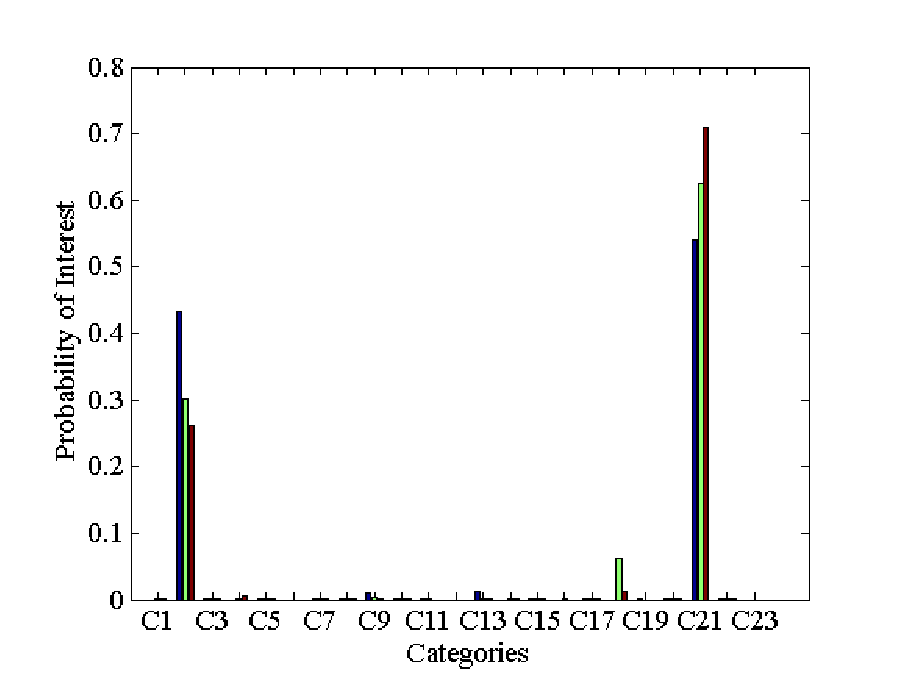
\includegraphics[width=11.5cm,height=5cm]{User2.eps} 
  \caption{Sample profile PMFs for three users from LiveLab smartphone traces.} 
       \label{fig:SampleProfile}
\end{figure}
 This key finding hinders the use of some metrics, such as Canberra
Distance and Jensen Shannon Divergence, with such sparse profiles due to the 
aforementioned infinite distance problem. 
%\par\end{flushleft}

Thus, we focus on the cosine (COS), Hellinger (HLNG), SVD and Vectorized cosine (VCOS) 
similarity metrics\footnote{Pearson correlation is not examined since it ranges 
from [-1, 1] and mapping for comparison to other metrics skew the similarity results.} 
to evaluate the pair-wise similarity for the $34$ LiveLab users,
which yields $561$ experiments. The outcomes of the four metrics
are shown, vs the experiment index, in the scatter plot depicted
in Fig.~\ref{fig:scatter}.
%
\begin{figure}[!tp]
  \centering
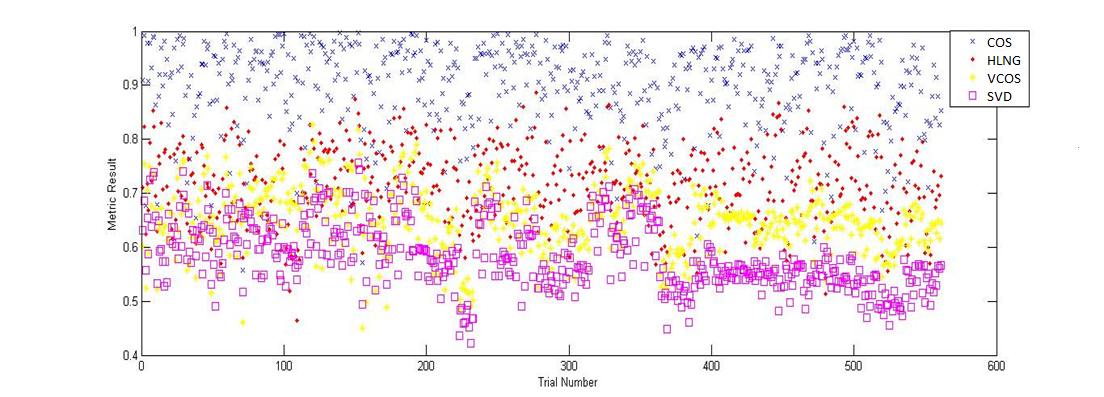
\includegraphics[width=12cm,height=5.3cm]{scatter.png}
%\vspace{-0.5cm}
 \caption{Metric indices for pair-wise similarity between LiveLab users.}
 \label{fig:scatter}
\end{figure}
%
First, it can be noticed from Fig.~\ref{fig:scatter} that cosine
and Hellinger similarity yield relatively higher metric values compared
to the VCOS and SVD for the same pair of users. This interesting result
confirms the intuition that temporal metrics are generally ``more thorough'' and, hence,
conservative in assessing mobile user similarity. Thus,
for a given threshold $T$ between $0$ and $1$, two users may be perceived ``similar'' using a non-temporal metric, yet, are deemed ``dissimilar'' using
a temporal metric. This is attributed to the fact that the temporal
profiles are generally more thorough since they naturally bear more details and dynamics 
than the non-temporal ones. This result is shown quantitatively in Table \ref{tab:Percentage-of-similar}.
\begin{table}
%\tabcolsep=0.05cm 
\caption{Percentage of similar users for all metrics for different similarity thresholds (T).}\label{tab:Percentage-of-similar}

\centering{}{} \label{tab:NonAndTemporal-Maj} %
\begin{tabular}{|l|l|l|l|l|l|l|l|l|l|l|}
\hline 
 & $T=$0.1 & 0.2  & 0.3  & 0.4  & 0.5  & 0.6  & 0.7  & 0.8  & 0.9  & 1\tabularnewline
\hline 
SVD  & 100  & 100  & 100  & 100  & 92.51  & 34.41  & 3.57  & 0  & 0  & 0\tabularnewline
\hline 
VCOS & 100  & 100  & 100  & 100  & 98.93  & 80.93  & 18.36  & 0.3565  & 0  & 0\tabularnewline
\hline 
Hellinger & 100  & 100  & 100  & 100  & 99.82  & 92.87  & 61.5  & 13.37  & 0  & 0\tabularnewline
\hline 
Cos & 100  & 100  & 100  & 100  & 100  & 99.47  & 97.33  & 89.13  & 59.18  & 0\tabularnewline
\hline 
\end{tabular}
\end{table}
The table shows that VCOS and SVD yield a lower percentage of similar users
than the cosine and Hellinger metrics, hence, they are more conservative. 
Second, the Hellinger metric may be perceived as a balance between both 
paradigms, since it is found to be closest to the average of the four 
metrics \cite{Mai13}. Although this demonstrates the potential of Hellinger 
similarity, it deserves further attention and analysis in future 
studies. Finally, the metrics studied and proposed here and 
the insights distilled open room for characterizing ``actual'' similarity, 
to serve as the ground truth in future work. 
%In addition, further analysis is needed to 
%contrast the HLNG and VCOS metrics to ``actual'' similarity (ground truth), 
%which is an important direction for future research.

Based on the above observations, we envision two similarity
assessment paradigms, namely macroscopic (non-temporal based) and
microscopic (temporal-based), which can serve as building blocks for 
two-stage similarity assessment.\\
\textit{Macroscopic assessment:} quantifies
similarity between two vector-based, non-temporal profiles. Evidently,
it is simpler and faster, with low-computational burden, yet, somewhat loose. Hence, it can 
serve as a first step ``coarse-grained'' similarity filter.\\
%This paradigm resembles getting to know a person quickly, yet, superficially.\\
\textit{Microscopic assessment:} scrutinizes similarity between two
matrix-based temporal profiles. Unlike the first paradigm, it is
more conservative in declaring similarity at the expense of more
complexity and, hence, being slower. It serves as a second step ``fine-grained'' 
similarity filter.

In the next section, we shift our attention to knowledge sharing between similar users.

%**********************************************************************************
\vspace{-1.0 cm}
\section{Knowledge Sharing in Opportunistic Social Networks}
\vspace{-0.3 cm}
In the rest of the paper, we shift our attention to knowledge sharing between similar users. Our prime focus is to introduce a novel mathematical framework, establish fundamental limits, as opposed to designing and implementing specific knowledge sharing schemes, which constitute an interesting topic of future research. This framework lays the basis for assessing the merits of future knowledge sharing and delay-tolerant forwarding policies in opportunistic social networks.

In particular, we characterize, with the aid of information theory, the amount of knowledge a user can extract in an opportunistic encounter, coined knowledge gain (KG), and the maximum amount of knowledge available for a user in the network, coined knowledge limit (KL). The use of modeling abstractions to study the formation, dynamics and evolution of social networks is not new. For instance, graph theory has been employed extensively  in social networks to model patterns of networks, clustering, homophily and basic concepts like centrality and connectedness,, e.g., \cite{graph1,graph3}. In
addition, random graph theory has been employed to model social network formation, evolution and growth, e.g., \cite{erdos,graph2}, among other topics. However, to the best of the authors' knowledge, employing information-theoretic tools to model knowledge sharing in opportunistic, mobile social networks has not been explored before.

%In this paper and after quantitatively assessing the similarity between mobile users given non-temporal or temporal profiles, we wish to take a look and investigate the collective knowledge available in an similarity-based opportunistic network. Modeling the user as a random variable opens ample room for using Information theory tools to measure different knowledge levels in the network. Section 1 introduces the system model in which we build our investigation upon. We then take a look about different performance metrics used to assess different forwarding schemes. We then introduce the Information-theoretic framework used to study the system at hand. We define novel concepts such as Knowledge Gain per encounter, Knowledge Limit and Overhead per encounter in Section 2. We then introduce two profile dissemination policies namely Mine Only and Mine Plus Others'. In Section 3, we investigate two network topologies: directly connected and indirectly connected topology. We model the users using the LiveLab \cite{data} data traces. We also investigate the previously mentioned topologies in a stationary scenario and using InfoCom 2005 \cite{infocom} mobility traces in a mobile scenario.

%%%%%%%%%%%%%%%%%%%%%%%Profile Structure & Management%%%%%%%%%%%%%%%%%%%%%%%%%%%%%%%
%\section{Performance Metrics for Information Dissemination Policies}
\vspace{-0.5 cm}
\subsection{Network Model and Assumptions}
\vspace{-0.2 cm}
The notion of a ``network'' here, that is, nodes exchanging information, 
is established solely based on pair-wise similarity, according to Section 3.
Thus, if a group of users in an opportunistic encounter, are all dissimilar, then there is no 
network, since no knowledge sharing will follow. The scenario of interest is the one that involves a subset of similar users which triggers tips exchange. Accordingly, we focus on a group of nodes where all nodes are pair-wise similar.
  
We model an opportunistic encounter of $M$ similar users as a wireless ad hoc network. We assume that each user is similar to all other users in the network. Each user has its own non-temporal profile vector, or multiple row vectors across the temporal dimension, modeled as a probability distribution across different categories as described in Section 3.1. Each user is assumed to have a table of recommendations that stores {\it tips} (knowledge) for sharing with similar users, e.g., upcoming event(s), bestsellers, site visits, etc. We assume that the users leverage short-range wireless communication technologies with fixed transmission power (i.e. the circular disk model), e.g., Wi-Fi or Bluetooth, and, hence, medium access issues are resolved using these protocols.

In this section, we wish to address two fundamental questions pertaining to knowledge sharing:\\
%\begin{itemize}
{\bf 1.} For an arbitrary user $i$, what is the maximum amount of knowledge available for this user (fundamental limit) in a given similarity-based opportunistic encounter (network)?\\
{\bf 2.} For user $i$, what is the amount of knowledge gain that is achievable, i.e. the user can actually reap from similar users in the network, using a specific knowledge sharing policy?
%\end{itemize}

Towards this objective, we introduce, next, terminology and mathematical definitions.
%Towards this objective, we introduce next a novel, information-theoretic framework for opportunistic, mobile social networks. We first start by introducing terminology and mathematical definitions.

%The $M$ nodes happened to meet opportunistically in a place e.g. super market, museum, club, etc. In this similarity-based network, the nodes don't exchange tips unless they are deemed similar. We measure the similarity between nodes by the classic cosine similarity or a variation of this metric between the PMFs of the users. We also assume that the probabilistic characteristics of the information tips that a user has are similar to the probabilistic characteristics of the user's behaviour captured via his/her interests and experiences (same first and higher order PMFs).\\

%For this model, and using different dissemination policies we wish to assess quantitatively the performance of the different forwarding policies through different metrics that we will discuss in detail shortly.
%An effective dissemination policy would disseminate one's tips to all similar nodes in the network without incurring a large overhead given energy constraints.

%
%\subsection{Performance Metrics}
%\begin{itemize}
%\item Delivery Percentage: If there are $k$ similar users to a certain user, an optimal dissemination policy would disseminate one's tips to all the $k$ users. In general the delivery percentage is defined as the number of similar users reached $k\prime$ out of the $k$ similar users. We will show later that this resembles all users achieving their Knowledge Capacity.
%\item Average cost: the cost in our context is the average hop count the tip takes to reach the destination.
%\item Forwarding Efficiency: is defined as dividing the delivery percentage by the average cost.
%\item Knowledge Gain: will be discussed in detail in the next section.
%In the next section, we will introduce the Information-theoretic framework that will enable us to model most of the aforementioned metrics in an Information-theoretic fashion. For the next sections we will assume a mobile user $X$ is a random variable that has a discrete probability mass function (PMF). It is noted that modelling the mobile user as a random variable opens ample room for the use of Information theory as atool in characterizing notions such as Knowledge Gain, Knowledge Capacity and Overhead as follows.
%\end{itemize}
%
\vspace{-0.5 cm}
\subsection{Knowledge Limit vs. Knowledge Gain}
\vspace{-0.2 cm}
In this section, we introduce two new concepts that are fundamental to the analysis that follows, namely the knowledge 
limit and knowledge gain.

\begin{defn}
The Knowledge Limit ($KL_i$) is defined, for an arbitrary user $i$, as the maximum amount of knowledge that is available for user $i$ to extract from similar users in a given network.
\end{defn}

\begin{defn}
The Knowledge Gain ($KG_i$) is defined, for an arbitrary user $i$, as the amount of knowledge user $i$ can gain from similar users, using a specific knowledge sharing policy.
\end{defn}

It is straightforward to notice that $KG_i \le KL_i$ since the knowledge limit constitutes the upper bound on the knowledge that can be reaped out of the network, irrespective of the sharing policy. Inspired by the probability distribution definition of the user profile, we argue that probability- and information-theoretic tools would prove useful for modeling and analyzing the system at hand.

Next, we introduce the formal definition of the knowledge gain per encounter. We assume that user tips (typically stored in a table) follow a probability distribution similar to the user profile. This does not only facilitate the mathematical analysis but is also a reasonable assumption, since users tend to have more tips in life categories they are more interested in.
%
%\begin{itemize}
%\item Knowledge Capacity for a given user (KC): defined as an upper bound on the maximum amount of new information that a user can extract from the similar users in a given network.
%\item Knowledge Gain for a given user (KG): defined as the amount of new information that a user extracted from the similar users in a given network via a specific dissemination policy. Axiomatically, the Knowledge Gain is always less than or equal to the Knowledge Capacity.
%\end{itemize}

%Since our model is probabilistic in nature (i.e the users' profiles are represented by PMFs), we use Information theory tools as one way to quantify both aforementioned notions.
%
\vspace{-0.3 cm}
\subsubsection{The Knowledge Gain per encounter}
\vspace{-0.2 cm}
We recall from information theory that the Entropy of a discrete-valued random variable $X$, denoted $H(X)$, represents a measure of the ``uncertainty'' which also represents the amount of information this random variable bears \cite{cover}. Given our assumption that the user recommendations/tips follow the same probability distribution as the user profile, tips can be modeled as a discrete random variable, $X$. Accordingly, $H(X)$ 
quantifies the amount of information (knowledge)\footnote{We use the terms Knowledge and Information interchangebly in this paper.} the user has. This model opens room for formally defining the newly introduced concepts of knowledge limit and gain.

First, we consider a toy example of an ``opportunistic encounter'' that involves only two users within the wireless communication range of each other. The two users have tips probability distribution vectors, denoted $X$ and $Y$. Assume users $X$ and $Y$ meet opportunistically and are deemed similar\footnote{We abuse notation and use the tips PMFs, $X$ and $Y$, to refer to the users as well.} , according to Section 3. Thus, they start exchanging informative tips. Based on simple entropy relationships,
%, depicted in the basic Venn diagram shown in Fig. ~\ref{fig:KGEncounter}
we distinguish three types of ``knowledge'' quantities (tips):\\ 
%
%Using our Assumption stated earlier that the probabilistic characteristics of the tips are the same as the probabilistic characteristics as his/her behaviour. We can use the information-theoretic entropy to help us quantify both Knowledge Gain and Knowledge Capacity.\\
%If we have two users $X$ and $Y$ who happen to opportunistically meet according to the similarity based opportunistic network that was described earlier and are deemed similar, they can now exchange tips.
%Using Information theory, we can quantify three important quantities as indicated in Fig. ~\ref{fig:KGEncounter}
%\begin{itemize}
%\vspace{-0.2 cm}
1. Tips that user $X$ has but $Y$ does not: given  by $H(X|Y)$.\\
2. Tips that user $Y$ has but $X$ does not: given by $H(Y|X)$.\\
3. Tips that both users have: given by $I(X;Y)$, the mutual information between $X$ and $Y$ .
%\end{itemize}

%It is straightforward to map the first type of tips (KG for user $X$) to the conditional entropy, 
%$H(Y|X)$. Similarly, the KG for user $Y$ is given by $H(X|Y)$. $KG(X)$ can also be written as
Note that the first type of tips is the knowledge gain of $Y$. Second, the knowledge gained by user $X$ from $Y$ can be defined as
%
\vspace{-0.5 cm}
\begin{equation}
KG(X) = H(Y|X) = H(X,Y) - H(X)
\end{equation}
where $H(X,Y)$ is the joint entropy of the two random variables representing the users tips probability distributions.
%
%If $X$ and $Y$ are deemed similar and they exchange tips. From the point of view of $Y$, the new information he/she gained is the first part mentioned earlier. This part is $H(X|Y)$ i.e. the Entropy (uncertainty/information content) of user $X$ given $Y$. So, the Knowledge Gain (KG) for user $Y$ in this case is $H(X|Y)$. Along the same lines, for user $X$, $KG=H(Y|X)$.
%
%Using some basic definitions from Information theory, we can rewrite the KG for user $X$ as $H(X,Y)-H(X)$. This can be directly interpreted as the amount of joint info that both $X$ and $Y$ have minus the amount of info that $X$ has.
The third type of tips (common to both users), characterized as the mutual information $I(X;Y)$, constitutes the ``communication overhead'' since it is exchanged over the air despite the fact that it does not contribute to increasing the knowledge of $X$ or $Y$. This perfectly 
agrees with our assumption that the two users know nothing about each other, when they meet opportunistically, for the first time and, hence, this overhead is unavoidable.
%
%\begin{figure}[!tp]
%  \centering
 %   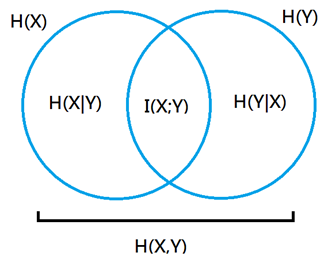
\includegraphics[width=6.5cm ,height=5cm]{figures_png/vennSimple}
 %   \caption{Characterizing knowledge gain and communication verhead for users $X$ and $Y$.}\label{fig:KGEncounter}
 %   \end{figure}

It is worth noting that the knowledge limit for user $X$ (or $Y$), in this toy example of two users, is equal to the knowledge gain. 
\vspace{-0.3 cm} 
\subsubsection{The Knowledge Gain Limit}
\vspace{-0.2 cm}
Based on the information-theoretic definitions of the KG and KL for a single encounter established in the previous section, we generalize the definition to characterize the knowledge limit for user $X_1$, without loss of generality, in an opportunistic encounter with $M-1$ other users, deemed similar to $X_1$, as follows: 
%Extending the insights that we formed about the KG quantity from the last subsection, we can now generalize the insights to get the general form for the Knowledge Capacity for a single user in a similarity-based opportunistic network of $M$ users.
%We can define the Knowledge Capacity(KC) for a single user $X_1$ as follows,
\vspace{-0.6 cm}
\begin{equation}
		KL(X_1) = H(X_1, X_2, X_3, ......, X_M) - H(X_1)
\end{equation}
%
%		$ | X_2, X_3, ......, X_M$ are similar to $X_1$
%\vspace{-0.6 cm}
which can be written as
\vspace{-0.4 cm}
\begin{equation}
KL(X_1) = H(X_2|X_1) + H(X_3|X_2,X_1) + .....+ H(X_M|X_{M-1}, ......, X_1).
%\nonumber
\end{equation}
%$ | X_2, X_3, ......, X_M$ are similar to $X_1$.
Thus, (3) asserts that the maximum amount of knowledge that user $X_1$ can extract from the network is simply the aggregate knowledge that all users have, after removing any redundant knowledge, which is represented by the joint entropy, $H(X_1, X_2, X_3, ......, X_M)$, less the knowledge user $X_1$ already has, that is, $H(X_1)$. We note that the KL characterization in (3) and (4) is general, valid for all network topologies and is independent of knowledge sharing policies.

%This powerful mathematical framework sets the stage to establish fundamental limits 
%and conduct analysis of diverse opportunistic social network settings under two 
%knowledge forwarding policies. This is the subject matter of the next subsection.
%Using these information theoretic tools and defining two basic information dissemination policies, we delve into different network configurations and attempt to apply the aforementioned definitions on them in order to further study them.
%%%%%%%%%%%%%%%%%%%%%%%%%%%%%%%%%%%%%%%%%%%%%%%%%%%%%%%%%%%%%%%%%%%%%%%
\vspace{-0.5 cm}
\subsection{Knowledge Sharing: Fundamental Limits and Policies}
\vspace{-0.2 cm}
We utilize the basic definitions introduced in the previous section to establish the KL of an arbitrary user in diverse scenarios as well as its KG, under two sample knowledge sharing policies:
i) Send my tips only, or ``{\it Send Mine Only}'', whereby a user sends only own 
tips to a similar, directly encountered user and ii) Forward my tips and others, or ``{\it Forward Mine Plus Others}'', whereby a user forwards own tips along with those acquired from others in previous encounters.

%Throughout the network model that we explained earlier, we can think of two extreme tips' exchange policies per encounter. Of course as explained earlier, the tips exchange occur only if the two users are deemed similar.
%\begin{itemize}
%\item Forward My Tips Only: or "Forward Mine Only" In this policy if the two users are similar, each one sends his/her own tips only.
%\item Forward My Tips and others: or "Forward Mine Plus Others'" In this policy if the two users are similar, each one sends his/her tips and the tips that he/she acquired from previous encounters.
%\end{itemize}
It is worth noting that these two policies are mere examples to illustrate the concept, however, other policies could be introduced and analyzed using the proposed model.
%Of course one can think of other policies or derivative policies from the previous two policies.
For instance, a user could forward own tips along with a subset of others' tips based on some criteria. This gives rise to a family of knowledge sharing policies that deserves a comprehensive analysis, to assess their merits and potential trade-offs, which lies out of the scope of this work. 
%Another hybrid policy would be forward My Tips only with probability $p$ and forward mine plus others with probability $1-p$.
%Our main focus in this work is to analyse the network dynamics for the two main dissemination policies: Forward Mine Only and Forward Mine Plus Others.
%
%%%%%%%%%%%%%%%%%%%%%%%%%%%%%%%%%%%%%%%%%%%%%%%%%%%%%%%%%%%%%%%%%%%%%%%%%%%%%%%%%%%
%\section{Similarity Based Network Analysis for Different Scenarios}

Next, we shift our attention to quantify the KL and KG achievable by the two aforementioned knowledge sharing policies, under a variety of opportunistic network configurations. In particular, we consider two connectivity scenarios, namely single-hop and multi-hop scenarios. In addition, we consider two mobility scenarios, namely fixed topology (i.e. stationary or quasi-stationary users) and time-varying topology caused by the user's portability within the same area. 
%The latter case is based, in the performance analysis study, on real traces gathered throughout a conference, particularly, Infocom 2005 \cite{infocom}.  

%The network model described earlier may/may not incorporate a Mobility component. We need to study both stationary and mobile models since the nodes may be stationary or moving around in the network area. We will study both directly and indirectly connected networks as the proximity/topology of the nodes play an important role since the communication that occurs here is point to point. 
%%%%%%%%%%%%%%%%%%%%%%%%%%%%
%%Check
%%For simplicity here, we will assume all the nodes in the network are mutually similar to focus on the Knowledge related concepts.
%%%%%%%%%%%%%%%%%%%%%%%%%%%%
%
\vspace{-0.3 cm}
\subsubsection{Fixed Topology, Similarity-based Opportunistic Networks}
\vspace{-0.2 cm}
%\subsubsection{Data used for Experimentation}
%{\it A. Data used for Experimentation}\\
%For the Stationary Similarity-based Opportunistic networks and modeling the user as a Random Variable, we will be conducting our experiments using LiveLab data \cite{data} described earlier. The network consists of $20$ nodes;  $B00$, $B02$, $B03$,
%$B04$, $B05$, $B06$, $B07$, $B08$, $B09$, $B10$, $B11$, $D00$, $D01$, $D02$, $D03$, $D04$, $D05$, $D06$, $D07$ and $D08$. We shall investigate the cumulative knowledge gain after each encounter and whether the gain will reach capacity or not and how many encounters shall it take to reach capacity.
%
%\subsubsection{ Stationary, Single Hop Network:}
%%%%%%%%%%%%%%%%%%%%%%%%%%%%%%%%%%%%%%%%%%%%%%%%%%%%%%%%%%%%%%%%%%%%%%%%%%%%
\noindent {\it A. Single-hop Networks}\\
Under this setting, the users may be stationary, quasi-stationary or portable, yet, each
node remains one-hop away, from all other nodes, all the time. 
%Thus, the nodes' movement does not alter the network topology, which always remains a full mesh. 
%Moreover, all nodes lie within the communication range of each other, that is, each node is a single hop away from all other nodes. 
For this setting, we can easily characterize the knowledge limit, as in (3), and, further, prove that the knowledge gain will attain the limit. This is in complete agreement with intuition since any node can take turn to exchange tips with all other nodes directly reachable. Thus, ``all'' knowledge that is available for any node in this network, can be fully reaped. 
%The interesting question here is: how long does it take to fully acquire this knowledge? It can be easily proven that it grows linearly with the network size, $M$, as confirmed by simulations which reveal interesting insights discussed in Section 4.4.
%
%Simply, since all nodes are in the same communication range of all other nodes, any node will be able to encounter any other node and extract its information, and if we assume that all nodes are mutually similar, the additive knowledge Gain will simply yield the Knowledge Capacity and this can be shown shortly.\\
This result is established for the {\it Send Mine Only} (SMO) policy in the following proposition.
%
%\begin{itemize}
%\item{Stationary Directly Connected (Single Hop) Network - Forward Mine Only:}
%in this network all nodes are in each others' range and if two users are deemed similar, each user exchanges only his/her tips.
%We now present a theorem and its proof suggesting that all nodes can achieve knowledge capacity.
%
\vspace{-0.2 cm}
\begin{prop}
For single-hop networks, an arbitrary node can achieve its knowledge gain limit using the {\it SMO} policy.
\end{prop}
%
\vspace{-0.5 cm}
\begin{proof}
Without loss of generality, we assume that node $X_1$ encounters other nodes in an ascending order of their IDs. Under the {\it Send Mine Only} policy, 
%shown in Fig.~\ref{SSHPNet}, 
the cumulative knowledge gain for node $X_1$, $KG(X_1)$, after receiving tips from all other nodes $X_2, X_3, X_4,...., X_M$ in turn, is given by $H(X_2|X_1) + H(X_3|X_2,X_1) + .....+ H(X_M|X_{M-1}, ......, X_1)$, which is the same as $KL(X_1)$ in (4). 
%It is straightforward to notice that this summation is itself $KL(X_1)$, given in (3). 
The same argument can be applied to all other nodes in the network which proves the result.
%$H(X_1, X_2, X_3, ......, X_M) - H(X_1)= KL(X_1)$. 
%The same can also be applied to any other node and along the same lines we can prove that it can achieve its knowledge capacity.\\
%
%\begin{figure}[!tp]
%\centering
%    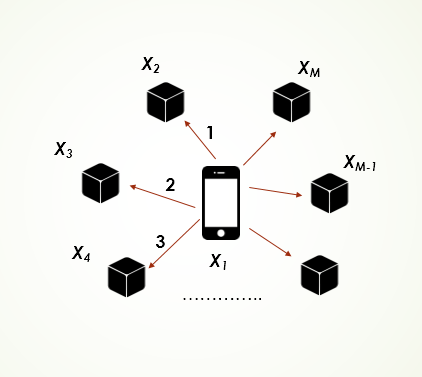
\includegraphics[width=8cm ,height=5.5cm]{figures_png/SSHPNet}
%    \caption{$X_1$ encounters enumerated.}\label{fig:KGEncounter}
%    \label{SSHPNet}
%\end{figure}
%
\end{proof}

%\vspace{-0.4 cm}
%\begin{cor}
%If there is at least one node that is unreachable from the rest of the network and has at least one unique tip (that is not %available at any other node), then $KG(X_1) < KL(X_1)$.
%\end{cor}
%\vspace{-0.2 cm}
%The proof is straightforward and is left as an exercise to the reader.\\
%
%%%%%%%%%%%%%%%%%%%%%%%%%%%%%%%%%%%%%%%%%%%%%%%%%%%%%%%%%%%%%%%%%
%\begin{theorem}
%If there is at least one node isolated from the rest of the a directly connected network that has at least one new tip (piece of information), $KG(X_1) \leq KL(X_1)$.\\
%\end{theorem}
%\begin{proof}
%%\textit{Proof:}
%Without loss of generality, we will assume that node $X_1$ will encounter other nodes in the network in an increasing order of node id and we assume a Forward Mine Only Policy. If node $X_M$ is isolated and can't be reached. So, the cumulative knowledge gain for node $X_1$, $KG(X_1)$, according to meeting nodes $X_2, X_3, X_4,...., X_{M-1}$ will be $$H(X_2|X_1) + H(X_3|X_2,X_1) + .....+ H(X_{M-1}|X_{M-2}, ......, X_1)$$ and this summation is missing the last term $H(X_M|X_{M-1}, ......, X_1)$ and since the entropy value is always greater than or equal zero so 
%$KG(X_1) <  KL(X_1) $.
%\end{proof}
%
As indicated earlier, one of the fundamental issues in our study is how long does it take a user to attain the knowledge limit. This is directly related to the number 
of exchanges needed to attain the KL. Under the {\it Send Mine Only} policy and assuming that each node has at least one unique tip to contribute to the knowledge in the network, then it is straightforward to show that the worst-case number of exchanges needed for an arbitrary node to attain the KL is simply $(M-1)$, that is, $O(M)$.
%%%%%%%%%%%%%%%%%%%%%%%%%%%%%%%%%%%%%%%%%%%%%%%%%%%%%%%%%%%%%%%%%%%%%%%%%%%%%
%\item{Stationary Directly Connected (Single Hop) Network - Forward Mine Plus Others':}

Next, we shift our attention to quantify the KG of single-hop networks, under the {\it Forward Mine Plus Others} (FMPO) sharing policy. Thus, a user shares not only its own tips but also tips collected from previous encounters, denoted by the subscript $p$. We prove in the following proposition that the knowledge limit is also attainable using the FMPO policy.
%in this network all nodes are in each others' range and if two users are deemed similar, each user exchanges his/her tips and the tips he/she has extracted from previous encounters. We model previous tips by subscript $p$.

%For the Stationary Directly Connected (Single Hop) network, and using Mine Plus Others' forwarding scheme, we can also show that any node can achieve the Knowledge Capacity.\\
%\textit{Example:}In a network of $4$ nodes ($X_1, X_2, X_3, X_4$), if we use a Mine Only forwarding scheme, $X_1$ will have to make $3$ encounters with $X_2, X_3$ and $X_4$ to reach its Knowledge Capacity. If we use a Mine Plus Others' forwarding scheme as shown in Fig. $X_1$ will reach the capacity in $2$ encounters.\\
%
\vspace{-0.2 cm}
\begin{prop}
For single-hop networks, an arbitrary node achieves the knowledge gain limit using the {\it FMPO} policy.
\end{prop}
%
\vspace{-0.5 cm}
\begin{proof}
Without loss of generality, we assume that each node starts off with its own knowledge only and node $X_1$ encounters all other nodes in an ascending order of their IDs. The knowledge exchange goes over multiple rounds whereby in the first round, for instance, the following exchanges take place in parallel: $X_1 \leftrightarrow X_2$, $X_3 \leftrightarrow X_4$, $X_5 \leftrightarrow X_6$, etc. Thus, $KG(X_1)$ based on encountering nodes $X_2, X_3, X_4,..., X_M$ in turn, is given by
\begin{equation}
KG(X_1) = H(X_2, |X_1) + H(X_3, \vec{X_{3p}}|X_2, X_1) + H(X_4, \vec{X_{4p}}|X_3, \vec{X_{3p}}, X_2, X_1)+.....
\nonumber
\end{equation} 
\begin{equation}
\hspace*{-4 cm} + H(X_M, \vec{X_{Mp}}|X_{M-1}, \vec{X_{(M-1)p}} ,......, X_1)
\end{equation}
\noindent where $\vec{X_{ip}}$ are the previous encounters of node $X_i$. It is straightforward to notice that $\vec{X_{3p}} = X_4$ since $X_1$ pairs with $X_3$ after the first round of exchanges. By the same token,  $\vec{X_{4p}} = X_3, X_5, X_6$, since $X_1$ pairs with $X_4$ after two rounds of pairing and so on. Thus, substituting in (5) after $M/2$ rounds yields
%
\begin{equation}
KG(X_1) = H(X_2, |X_1) + H(X_3, X_4|X_2, X_1) + H(X_4, X_3, X_5, X_6|X_4, X_3, X_2, X_1)+.....
\nonumber
\end{equation} 
\begin{equation}
\hspace*{-5 cm} + H(X_M, \vec{X_{Mp}}|X_{M-1}, \vec{X_{(M-1)p}} ,......, X_1)
\end{equation}
Using the chain rule of entropies and expanding all terms in (6) yields some zero terms due to acquiring the same (redundant) knowledge from previous encounters. This, in turn, yields the KL in (4) and proves the result.
%
%It can be shown that each joint entropy term in (5) can be expanded, 
%e.g., $H(X_2, \vec{X_{2p}}|X_1)$ becomes $H(X_2|X_1) + H(\vec{X_{2p}}|X_2, X_1)$, where 
%the latter term (previous encounter tips of a node) would be redundant in some cases (acquired from earlier encounters) %and, hence, contributes zero to the KG. This, in turn, reduces (5) to the KL in (4) and proves the result.
%This reduces to the  KL in (3) and proves the result.
\end{proof}
%
It should be noted that once the conditioning, in the conditional entropy terms in the RHS, accommodates all nodes in the network, the incremental gain becomes zero and the node achieves its knowledge limit. In essence, the role of the previous encounters (appearing in the conditional entropy terms) is the sole contributor to the FMPO policy attaining the KL faster, compared to the SMO policy, which will be shown in Section 4.4. Apparently, this does not come 
for free since there is a fundamental trade-off between the cumulative KG after a number of encounters and the associated communication overhead which warrants attention in future research, especially in multi-hop networks. We prove next that the communication overhead of FMPO is greater than or equal to SMO, in single-hop networks.
%
\vspace{-0.2 cm}
\begin{prop}
For single-hop networks, the communication overhead under FMPO is greater than or equal to SMO.
\end{prop}
%
\vspace{-0.5 cm}
\begin{proof}
We consider an encounter beween two users, $X$ and $Y$. Generalizing to a sequence of encounters is straightforward. Denote the vector of previous encounters for $X$ and $Y$ by $\vec{X_p}$ and $\vec{Y_p}$, respectively.

Under the SMO policy, the communication overhead that $X$ incurs is the common knowledge (mutual information) between what $X$ sends (which is its knowledge only) and $Y$'s 
knowledge so far which is given by 
\begin{equation}
OH(X)_{SMO}=I(X;Y,\vec{Y_p}).
\label{overheadX}
\end{equation}
Similarly, the communication overhead from the perspective of user $Y$ is $OH(Y)_{SMO}=I(Y;X,\vec{X_p})$.

Under FMPO, the communication overhead is the same for both users and is given by
\begin{equation} 
OH(X)_{FMPO}=OH(Y)_{FMPO}=I(X,\vec{X_p};Y, \vec{Y_p}).
\label{overheadXY}
\end{equation}

The mutual information between two random variables $A$ and $B$ can be written as
\begin{equation} 
I(A;B)=H(A) + H(B) - H(A,B).
\label{mutInfoEqn}
\end{equation}
%\vspace{-0.4 cm}
Applying ~\eqref{mutInfoEqn} on ~\eqref{overheadX} yields
\begin{equation}
OH(X)_{SMO}= H(X)+H(Y,\vec{Y_p})-H(X,Y,\vec{Y_p}).
\label{Eqn.4}
\end{equation}
Applying ~\eqref{mutInfoEqn} on ~\eqref{overheadXY} yields
\begin{equation}
OH(X)_{FMPO}=OH(Y)_{FMPO}= H(X,\vec{X_p})+H(Y,\vec{Y_p})-H(X,\vec{X_p},Y,\vec{Y_p}).
\label{Eqn.3}
\end{equation}
Subtracting ~\eqref{Eqn.4} from ~\eqref{Eqn.3} yields 
\begin{equation}
OH(X)_{FMPO}-OH(X)_{SMO}=H(X,\vec{X_p})-H(X)-H(X,\vec{X_p},Y,\vec{Y_p})+H(X,Y,\vec{Y_p})
%H(Y,\vec{Y_p})-H(Y)-H(X,\vec{X_p},Y,\vec{Y_p})+H(X,\vec{X_p},Y).
\label{Eqn.5}
\end{equation}
Since $H(A,B) = H(A) + H(B|A) = H(B) + H(A|B) $, ~\eqref{Eqn.5} can be re-written as
\begin{equation}
OH(X)_{FMPO}-OH(X)_{SMO}=H(X)+H(\vec{X_p}|X)-H(X)-[H(\vec{X_p}|X,Y,\vec{Y_p})+H(X,Y,\vec{Y_p})] + H(X,Y,\vec{Y_p}),
\nonumber
\end{equation}
which reduces to 
\vspace{-0.5 cm}
\begin{equation}
OH(X)_{FMPO}-OH(X)_{SMO}=H(\vec{X_p}|X)- H(\vec{X_p}|X,Y,\vec{Y_p}),
\label{lasteqn}
\end{equation}
\begin{equation}
\hspace*{0.6 cm} \ge 0,
\label{ineq}
\end{equation}
where the inequality in~\eqref{ineq} follows since conditioning reduces entropy. This proves the result.
\end{proof}
%
%\vspace{-0.3 cm}
%\noindent \textbf{Example 1.} This example illustrates the KL achievability speedup under FMPO. Consider a network of $4$ users, $X_1, X_2, X_3, X_4$, going through two encounters as shown in Figs.~\ref{fig:SSHP(MO1)}(a) and (b), respectively. The two figures show the knowledge at a node before exchange (KBE) and the knowledge after exchange (KAE). It can be noticed from Fig.~\ref{fig:SSHP(MO1)}(b) that all nodes would reach their KLs after, only, two encounters, as opposed to $M-1$ encounters (three in this scenario) under the {\it Send Mine Only} (SMO) policy.
%
%\vspace{-0.3 cm}
%\begin{figure}[!bp]
%\centering
%    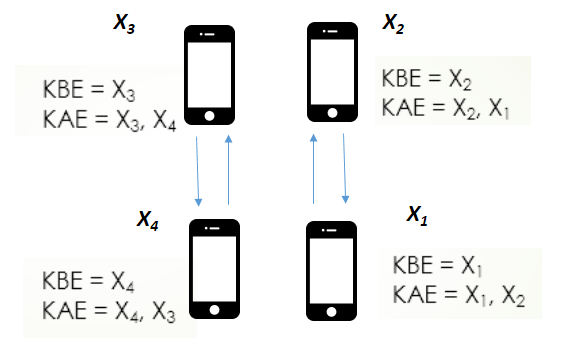
\includegraphics[width=8cm ,height=5cm]{figures_png/SSHP(MO1)}
%    \hspace {1 cm} 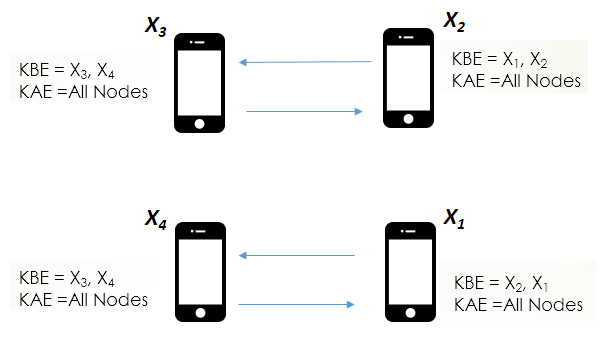
\includegraphics[width=8cm ,height=5cm]{figures_png/SSHP(MO2)}
%\centerline{(a) \hspace{9 cm} (b)}
%    \caption{Illustrating the KL achievability speedup using FMPO: (a) 1st encounter, (b) 2nd encounter.}\label{fig:SSHP(MO1)}
%    \label{SSHP(MO1)}
%\end{figure}
%
%
%
%\begin{figure}[!bp]
%\centering
%    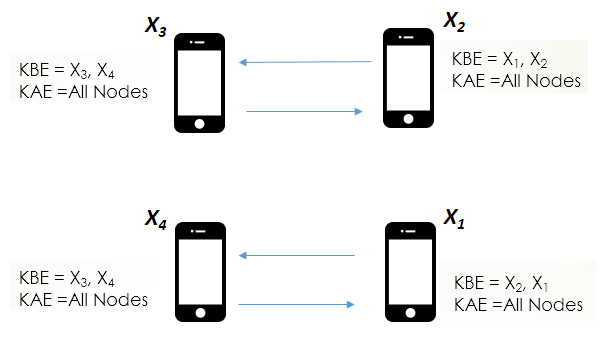
\includegraphics[width=8cm ,height=5.5cm]{figures_png/SSHP(MO2)}
%    \caption{A scenario for encounters (Second Step).}\label{fig:SSHP(MO2)}
%    \label{SSHP(MO2)}
%\end{figure}
%\vspace{-0.2 cm}
%\begin{figure}[htpb]
%\epsfysize 2.5in
%\centerline{\epsfbox{example2.eps} \epsfysize 2.5in \epsfbox{example3.eps}}
%\centerline{(a) \hspace{7.6 cm} (b)}
%\centerline{\epsfysize 2.5in \epsfbox{example4.eps}}
%\centerline{(c)}
%\vspace{-0.3 cm}
%\caption{Three Interference Scenarios with ten 8x8 MIMO links: (a) Low Interference, (b) Medium Interference, (c) High Interference}
%\end{figure}

%On the other hand, if we each node uses a Forward My Tips and others dissemination policy and if we assume that the system of the nodes will be exchanging tips for a while before a new node enters the network environment, then we have two extreme cases as follows.\\
%In the best case, where the new entering node named $X$ meets a node that has gathered all the tips in the system named $Y$, then the number of exchanges that $X$ needs to attain capacity is one, hence a complexity of $O(1)$.\\
%On the other hand, the worst case scenario is simply when no enough exchanges are done before node $X$ enters the system and this leads to the Mine plus others scheme falling back to the Mine Only scheme and the number of exchanges needed by $X$ to attain capacity will be $O(N)$.
%
%%%%%%%%%%%%%%%%%%%%%%%%%%%%%%%%%%%%%%%%%%%%%%%%%%%%%%%%%%%%%%%%%%%%%%%%%%%%%%%%
%\subsubsection{Stationary Indirectly Connected Network:} 
\vspace{-0.2 cm}
\noindent {\it B. Fixed Topology Multi-hop Networks}\\
Under this setting, we assume the network topology is connected and time-invariant where some nodes are multi-hop away from each other. In this case, the role of
the knowledge sharing policy stands out and affects whether a user can/cannot attain the KL.
%
%in this kind of network, not all nodes are in the same communication range of each other. If we take node $X_1$ for example, then in this kind of network it will have a subset of the $M$ nodes, say $N$ where $N<M$, in the same communication range or one hop away and the other $M-N$ nodes not reachable by $X_1$.\\
%Here the information dissemination policy plays an important role in whether or not a node attains the Knowledge Capacity.
%
%\begin{itemize}
%\item{Stationary Indirectly Connected (Multi-Hop) Network - Forward Mine Only:}

Next, we quantify the performance, and trade-offs, of the SMO and FMPO policies. In case of
%in this network shown in Fig.~\ref{SMHPNet}
SMO, the knowledge gain achieved by node $X_1$ is limited by the neighborhood size, $N$<$M$ which renders the KG strictly less than the KL. The following proposition establishes this result.
\vspace{-0.2 cm}
\begin{prop}
For fixed topology, multi-hop networks, the SMO knowledge sharing policy is not guaranteed to attain the knowledge gain limit, that is, $KG(X_1) \le KL(X_1)$ iff $N<M$.
\end{prop}
%\textit{Proof:}\\
%
\vspace{-0.4 cm}
\begin{proof}
Without loss of generality, we assume node $X_1$ communicates with other nodes in an ascending order of their IDs. The cumulative knowledge gain for node $X_1$, $KG(X_1)$, according to exchanges with neighbors $X_2, X_3, X_4,...., X_{N}$ is given by $H(X_2|X_1) + H(X_3|X_2,X_1) + .....+ H(X_{N}|X_{N-1}, ......, X_1)$. It is worth noting that the summation of non-negative conditional entropy terms is limited to $N<M$ nodes. It misses other non-negative terms involving the $M-N$ non-neighbors to $X_1$. Hence, it directly follows that $KG(X_1) \le KL(X_1)$, which proves the result.
%
%and this summation is missing the terms $H(X_{N+1}|X_{N}, ......, X_1)$ till $H(X_{M}|X_{M-1}, ......, X_1)$ and since these terms are entropy terms whose values are always greater than or equal zero so.
\end{proof}
%
\vspace{-0.5 cm}
It is worth noting that the special case of $N=M$, for all nodes, reduces to the single-hop network case where we have shown in Section 4.3.1.A that the KL is achievable under both knowledge sharing policies.
%
%The situation differs for example for any node that has all nodes in its range i.e., $N=M$. For this node, capacity will be achieved (all missing terms from the last proof will be added and the gain reaches capacity). 
%
An interesting, and somewhat surprising insight, which will be discussed later, is that nodes mobility can be leveraged to achieve the knowledge limit, even if $N<M$.

%\begin{figure}[!tp]
%\centering
%    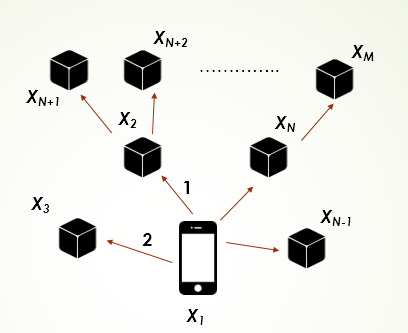
\includegraphics[width=8cm ,height=5.5cm]{figures_png/SMHP(MO)}
%    \caption{Fixed Topology Multi-Hop Network.}\label{fig:SMHP(MO)}
%    \label{SMHPNet}
%\end{figure}
%===========================================================================================
%\item{Stationary Indirectly Connected (Multi Hop) Network - Forward Mine Plus Others':}

Next, we focus on the performance of the FMPO knowledge sharing policy 
for fixed topology multi-hop networks. As expected, forwarding others tips opens room for a node to achieve its KL, even if $N<M$. The following proposition formally establishes this result. 
%we now study this network using a Forward Mine Plus Others' policy. If we assume multiple encounters with the same node is allowed and the neighboring nodes for $X_1$ collected the knowledge of non-neighbouring nodes for $X_1$, then $X_1$ can attain its knowledge limit. We now present this in the next proposition.
%
\vspace{-0.2 cm}
\begin{prop}
For fixed topology, multi-hop networks, an arbitrary node can achieve the knowledge gain limit using the FMPO knowledge sharing policy.
\end{prop}
%
%\textit{Proof:}
\begin{proof}
We provide an outline of the proof due to space limiations. Without loss of generality, we assume that each node starts off with its own knowledge only and $X_1$ encounters its single-hop neighbors in an ascending order of their IDs, while other neighbors have pair-wise encounters with other nodes in the network. The cumulative knowledge gain for node $X_1$, $KG(X_1)$, after meeting neighboring nodes $X_2, X_3, X_4,...., X_N$ is given by
\vspace{-0.2 cm}
\begin{equation}
KG(X_1)=H(X_2,|X_1) + H(X_3, \vec{X_{3p}}|X_2,X_1) + H(X_4, \vec{X_{4p}}|X_3, \vec{X_{3p}}, X_2,X_1)+.....
\nonumber
\end{equation}
\begin{equation}
\hspace*{-4.3 cm} + H(X_N, \vec{X_{Np}}|X_{N-1}, \vec{X_{(N-1)p}} ,......, X_1). 
\end{equation}
 At this point, two cases arise. First, if the previous knowledge vectors, $\vec{X_{ip}}$ $\forall i$, bear the ``forwarded'' tips from all non-neighboring nodes, namely $X_{N+1}, X_{N+2}, ......, X_M$, then it can be shown that the cumulative knowledge gain of $X_1$ becomes
%
\vspace{-0.4 cm}
\begin{equation}
KG(X_1)=H(X_1, X_2, X_3, ......, X_M) - H(X_1)= KL(X_1) 
\end{equation} 
%
\noindent which proves the result. Second, if the previous encounters do not cover knowledge from all non-neighbors, then this implies that node $X_1$ needs more time to attain $KL(X_1)$. Backed by network connectedness and unconstrained delay, $X_1$ can attain its KL almost surely via re-pairing with neighbors it has already parid with (to reap new knowledge acquired over time) until it acquires all missing knowledge from nodes out of its communication range.
%
%\noindent which attains the $KL(X_1)$. On the other hand, if the previous encounters do not cover tips from non-neighbors, then this implies that node $X_1$ needs more time to attain $KL(X_1)$, possibly via revisiting neighbors that it has already visited to acquire the missing knowledge from nodes out of its communication range, until it eventually reaches limit. 
%It should be noted that once the conditioning, in the conditional entropy terms in the RHS, accommodate all in the network, the incremental gain becomes zero and the node achieves its knowledge capacity.
%Of course once the right hand side of the given sign has the full list of the nodes in the network, the added gain will be zero and the node will have reached its Knowledge Capacity.
This proves the result.
\end{proof}
%\end{itemize}

%On the contrary, if the dissemination policy used in this network is Forward Mine Plus Others we can find best and worst cases scenarios.
%The best case for this situation happens when the $N$ neighbouring nodes have the knowledge (tips) of the non-neighbouring nodes. If that is the case and through using the Mine plus others policy, $X$ could attain the Knowledge Capacity.
%The worst case for this situation happens when the $M-N$ non neighbouring nodes for $X$ can't be reached by the $N$ neighbouring nodes and thus this case falls back to the Mine Only strategy in the last paragraph.
%The average case naturally happens when some of the non-neighbouring nodes are achievable and some aren't and in this case also $X$ can't attain Knowledge Capacity as well.
%%%%%%%%%%%%%%%%%%%%%%%%%%%%%%%%%%%%%%%%%%%%%%%%%%%%%%%%%%%%%%%%%%%%%%%%%%%%%%%%%%%%%5
%\subsubsection{LiveLab Results for Stationary Similarity-based Opportunistic Network }
\vspace{-0.5 cm}
\subsection{User Traces and Performance Results}
%\section{Real User Traces and Performance Results}
\vspace{-0.2 cm}
In this section, we support our theoretical findings with numerical results based on 
smartphone user profile traces \cite{data} and real-life user mobility traces, gathered at Infocom 2005 \cite{infocom,diot}.
\vspace{-0.3 cm}
\subsubsection{Single-hop Networks}
%\subsection{Fixed Topology, Single-hop Similarity-based Networks}
\vspace{-0.2 cm}
%
%After describing the different topologies for the similarity-based Opportunistic Network under investigation, we now present the results after incorporating 
%
In this section, we rely on real user traces, either for user behavior or mobility. For user behavior, we utilize digital footprint traces (interests) for $20$ smartphone users, over $V=24$ life categories, from the LiveLab project \cite{data}. 
%In this section, we assume stationary, or quasi-stationary, users and, hence, the network topology is a time-invariant full mesh. 
In order to quantify the knowledge limit and gain for an arbitrary user, we need to pre-process a huge amount of six month worth of interests data in two steps. First, we compute the joint probability mass function for the 20 users under investigation over the period from September 2010 to February 2011. Thus, we monitor the users' activities categorized under $24$ categories\footnote{The 24th category captures the case when the smartphone is off or not running any application.}, each second, and record their concurrent activities. Afterwards, we divide by the total duration of the six months to get the joint PMF. Next, we show the cumulative knowledge gain increase as the node under investigation encounters more nodes over time.
%===========================================================================================================
%\begin{itemize}
%\item Results for Stationary Directly Connected (Single-Hop)- Mine Only Network:

First, we present the performance results for a single-hop network under the SMO knowledge sharing policy. For the network of $M=20$ nodes discussed earlier, an 
arbitrary user can achieve the knowledge limit within $M-1=19$ encounters. This is shown in Fig.~\ref{fig:B00_SSHOP)} for three arbitrary users, namely $B00$, $B04$ and $D03$. It can be noticed that the cumulative knowledge gain is a non-decreasing function with time. On the other hand, the knowledge gain limit is shown as 
a horizontal solid line that is generally different from one user to another.
%
\begin{figure}[!tp]
\centering
    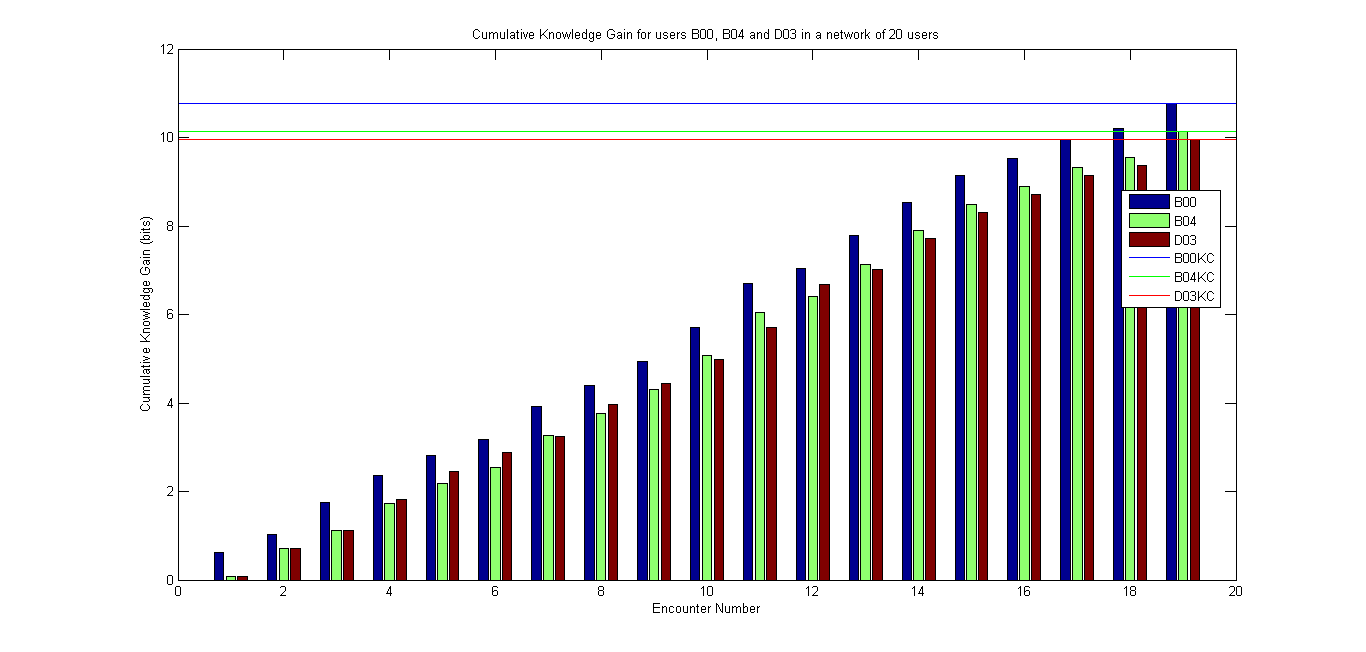
\includegraphics[width=10cm ,height=5.6cm]{figures_png/Fig5}
%    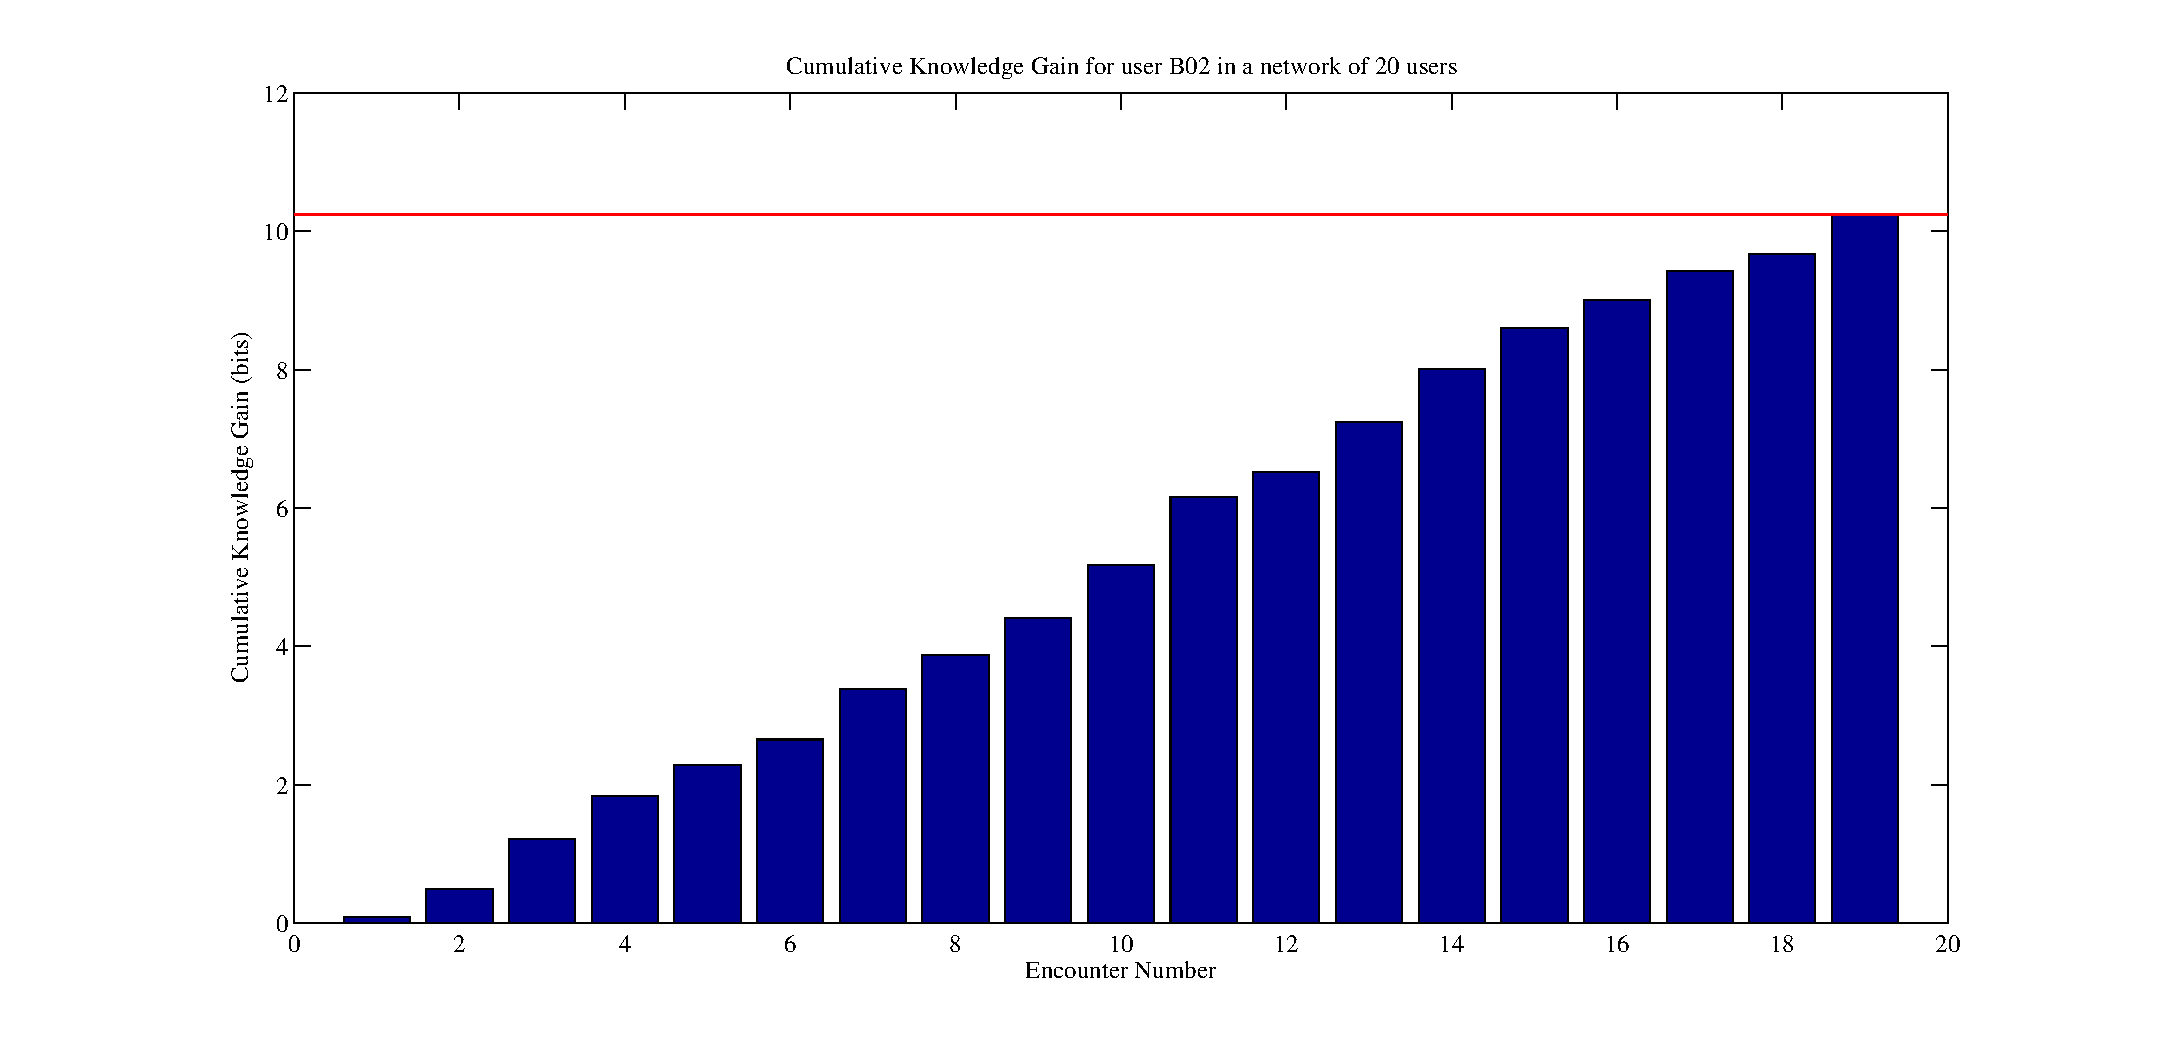
\includegraphics[width=8.1cm ,height=5.6cm]{figures_eps/B02_SSHOP}
%\centerline{(a) \hspace{9 cm} (b)}
%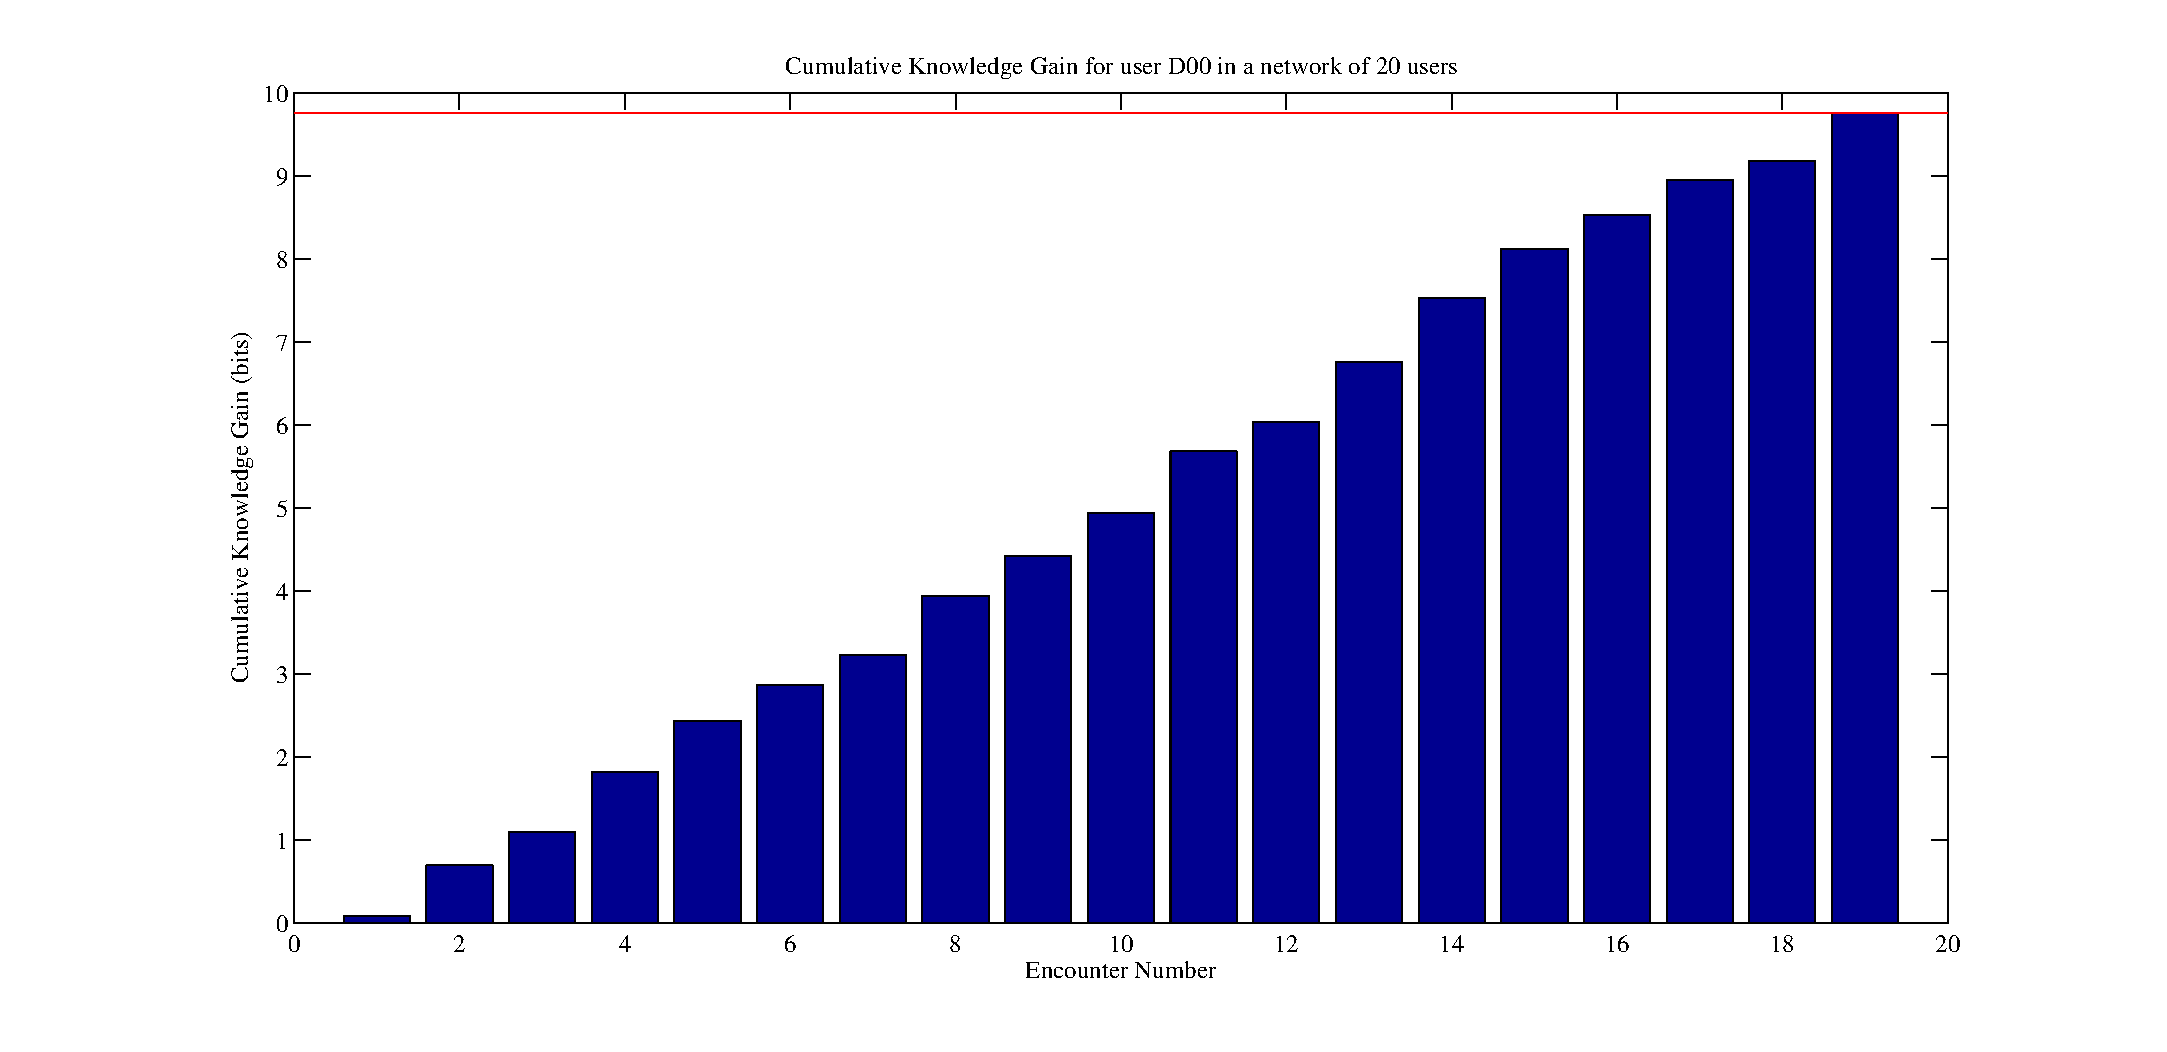
\includegraphics[width=8.1cm ,height=5.6cm]{figures_eps/D00_SSHOP}
%\centerline{(c)}
    \caption{Cumulative knowledge gain for three users in a single-hop network under SMO.}\label{fig:B00_SSHOP)}
\end{figure}
%
%\begin{figure}[!tp]
%\centering
%    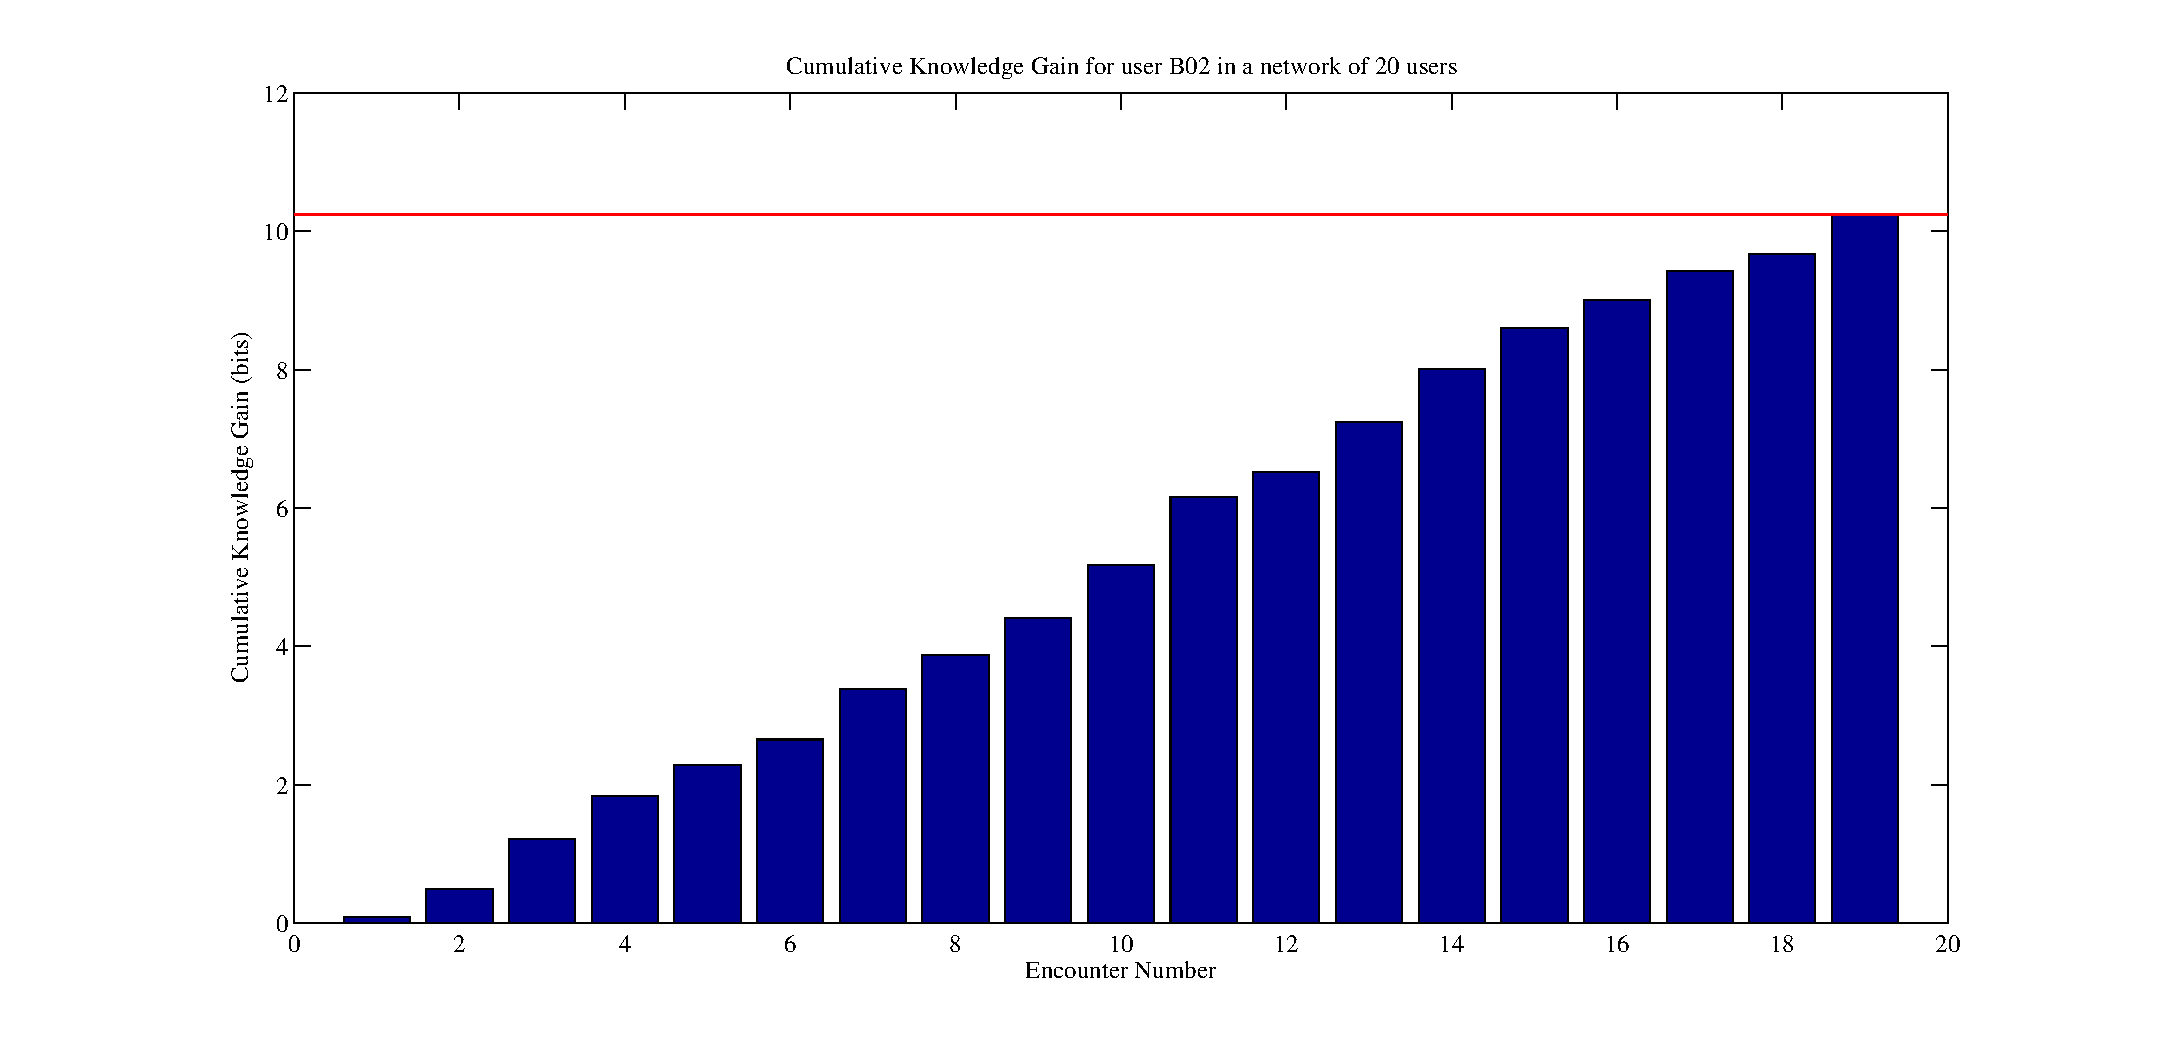
\includegraphics[width=12cm ,height=7cm]{figures_eps/B02_SSHOP}
%    \caption{Cumulative knowledge gain for user B02 in a fixed topology single-hop network under (SMO).}\label{fig:B02_SSHOP)}
%\end{figure}
%\begin{figure}[!tp]
%\centering
%    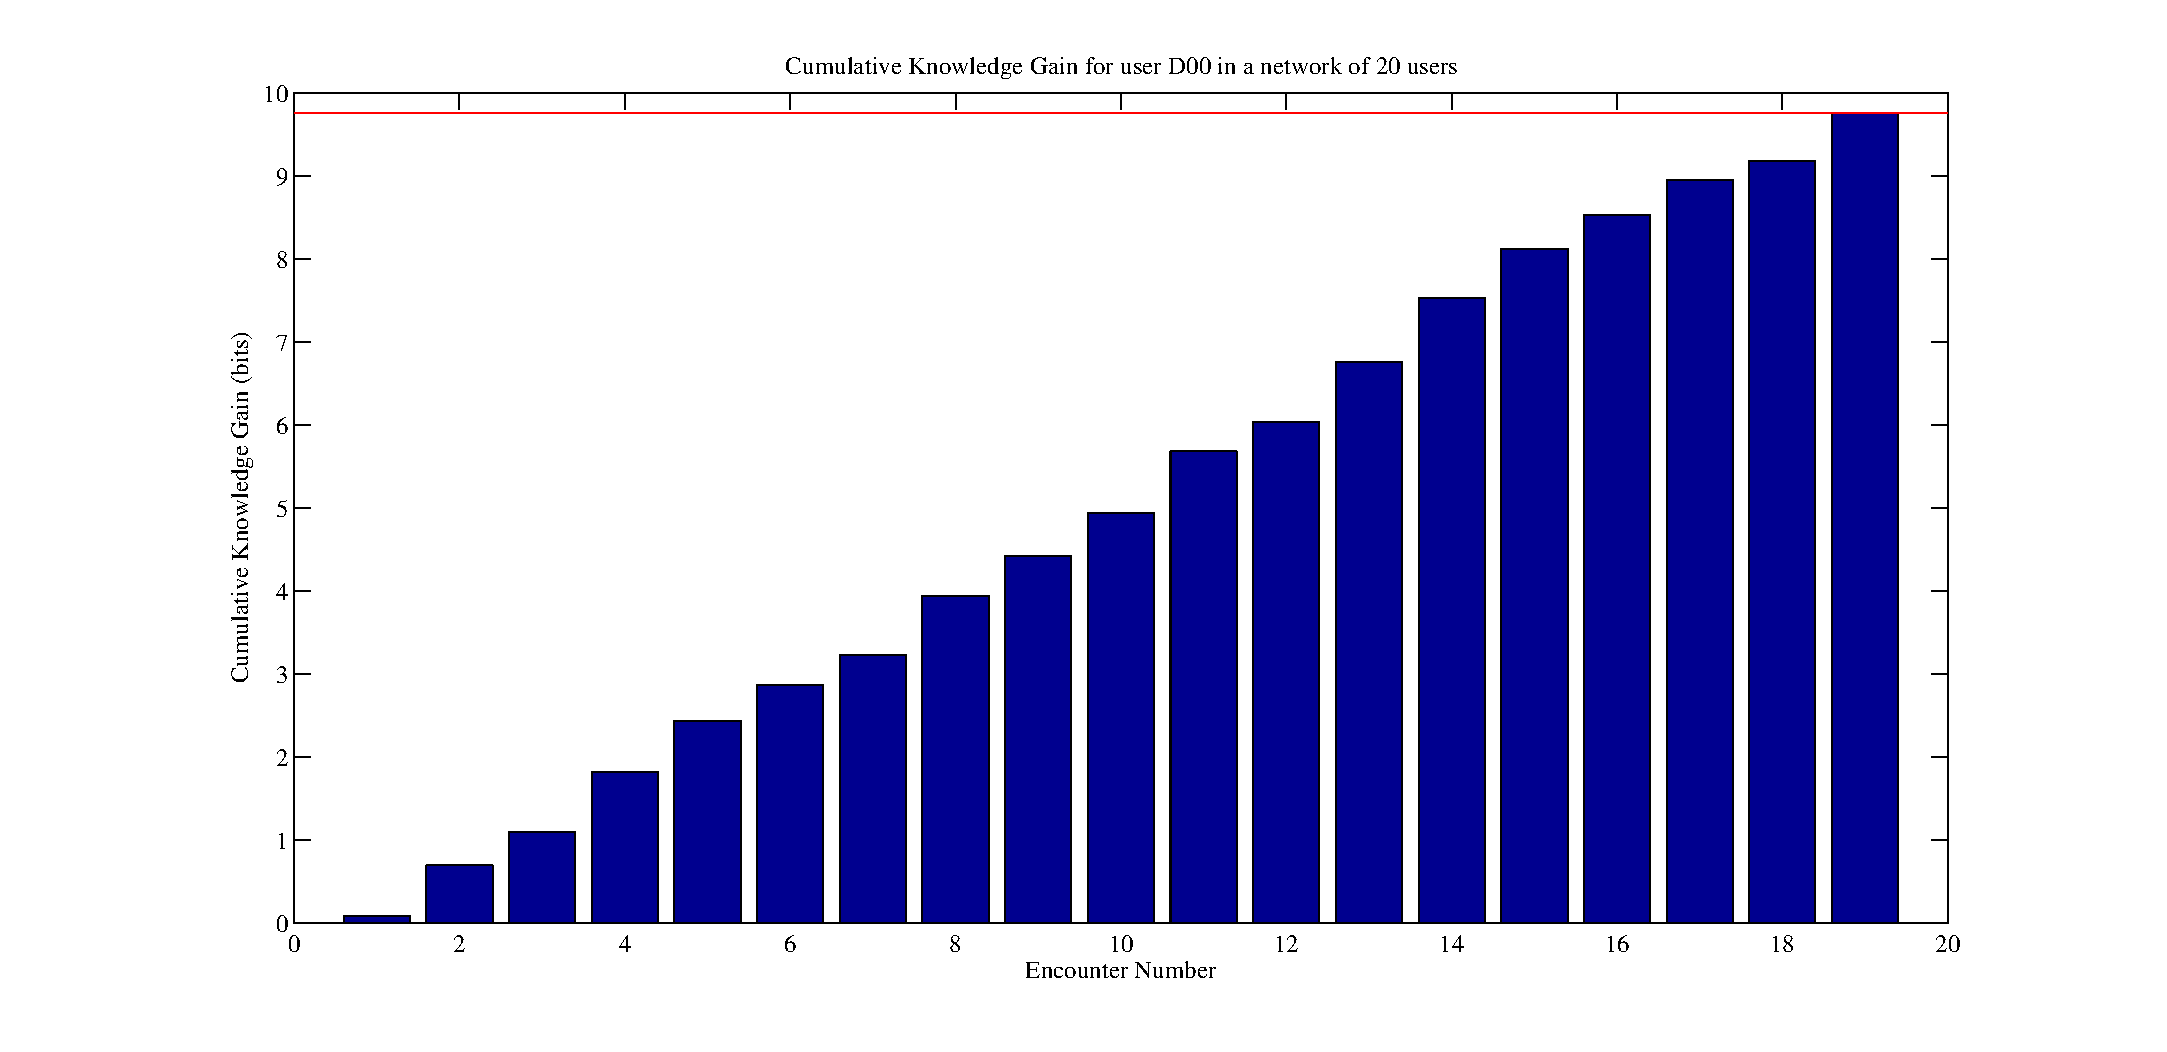
\includegraphics[width=12cm ,height=7cm]{figures_eps/D00_SSHOP}
%    \caption{Cumulative knowledge gain for user D00 in a fixed topology single-hop network under (SMO).}\label{fig:D00_SSHOP)}
%\end{figure}
%================================================================================================================
%\item Results for Stationary Directly Connected (Single-Hop)- Mine Plus Others' Network:

Next, we consider the same network setting, yet, employing the FMPO policy.
Based on Proposition 2, we show that, for this type of networks, all nodes achieve the knowledge limit using the FMPO policy, yet, faster than SMO, i.e. in less encounters due to sharing the tips of others. This valuable insight is confirmed for users $B00$, $B04$ and $D03$ in Fig.~\ref{fig:B00_SSHOP(MO)}.
%
\begin{figure}[!bp]
\centering
    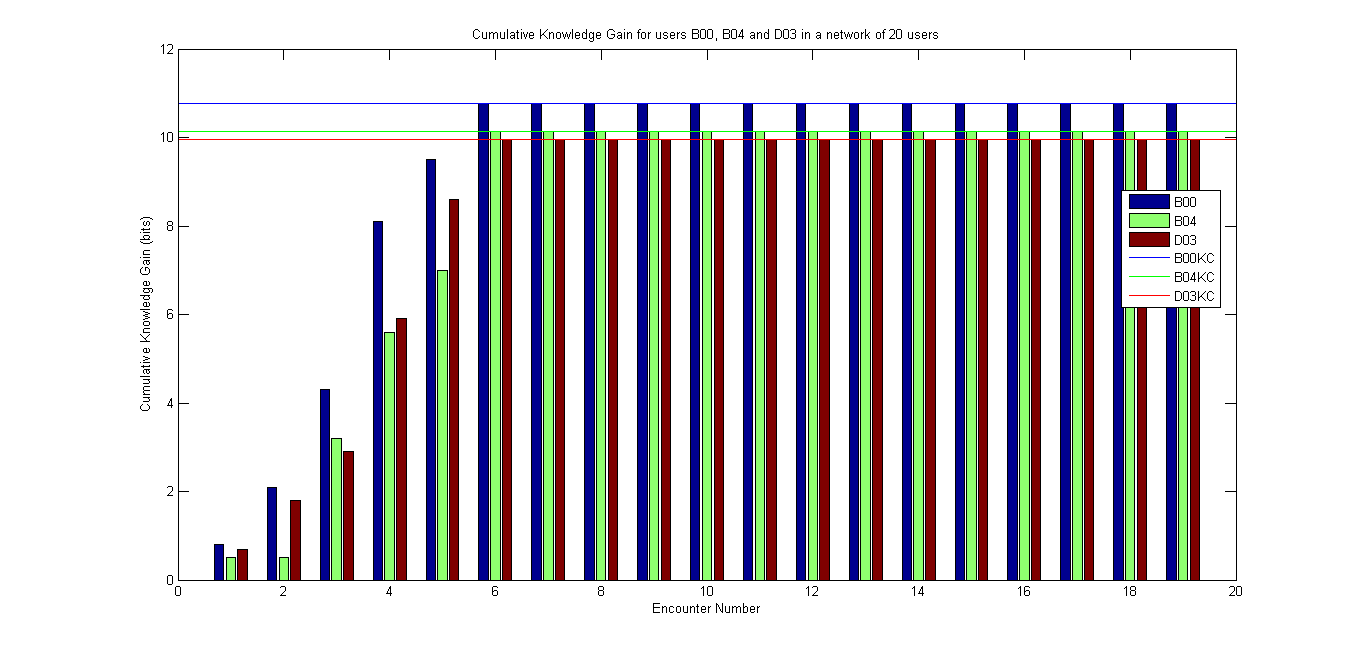
\includegraphics[width=10cm ,height=5.6cm]{figures_png/Fig6}
%    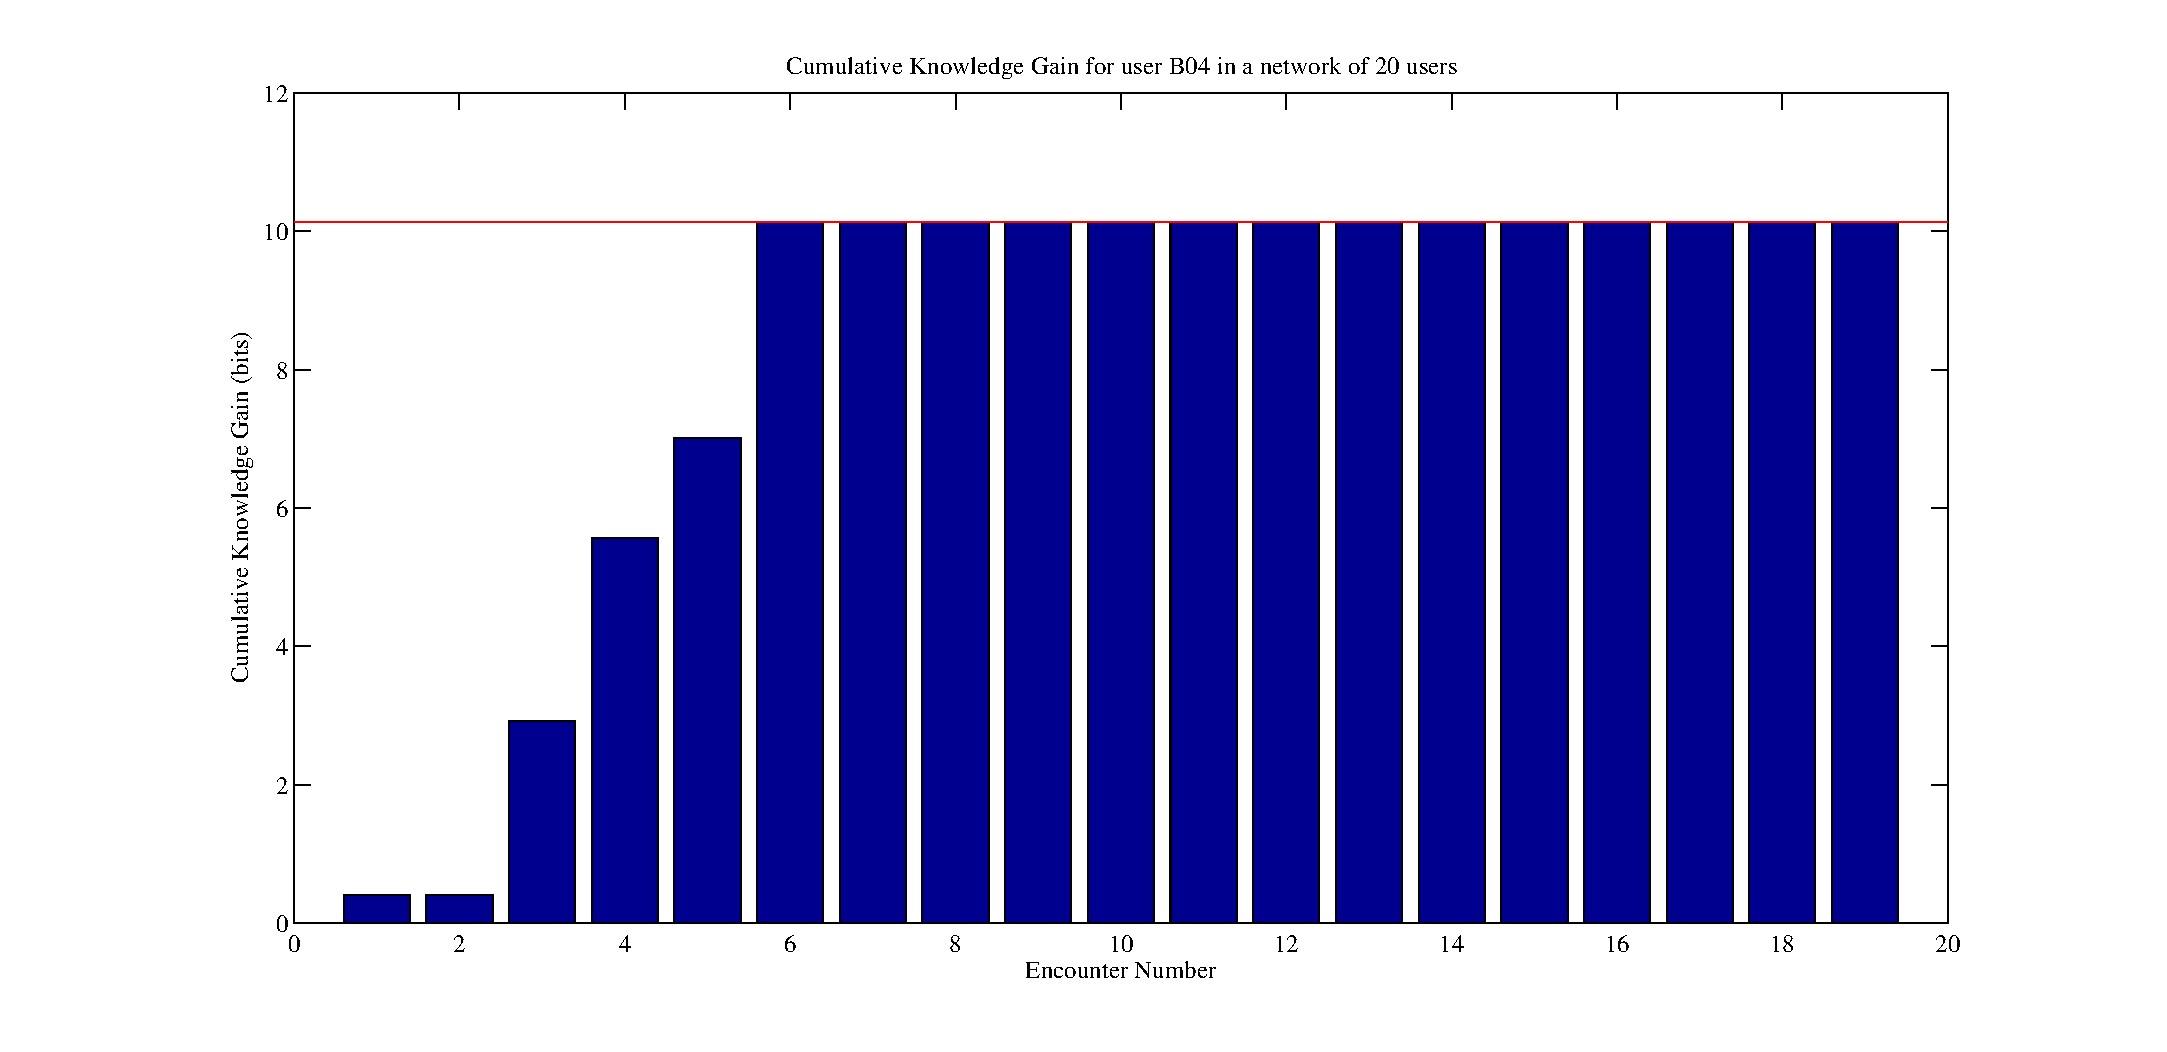
\includegraphics[width=8.1cm ,height=5.6cm]{figures_eps/B04_SSHOP_MO.eps}
%\centerline{(a) \hspace{9 cm} (b)}
%  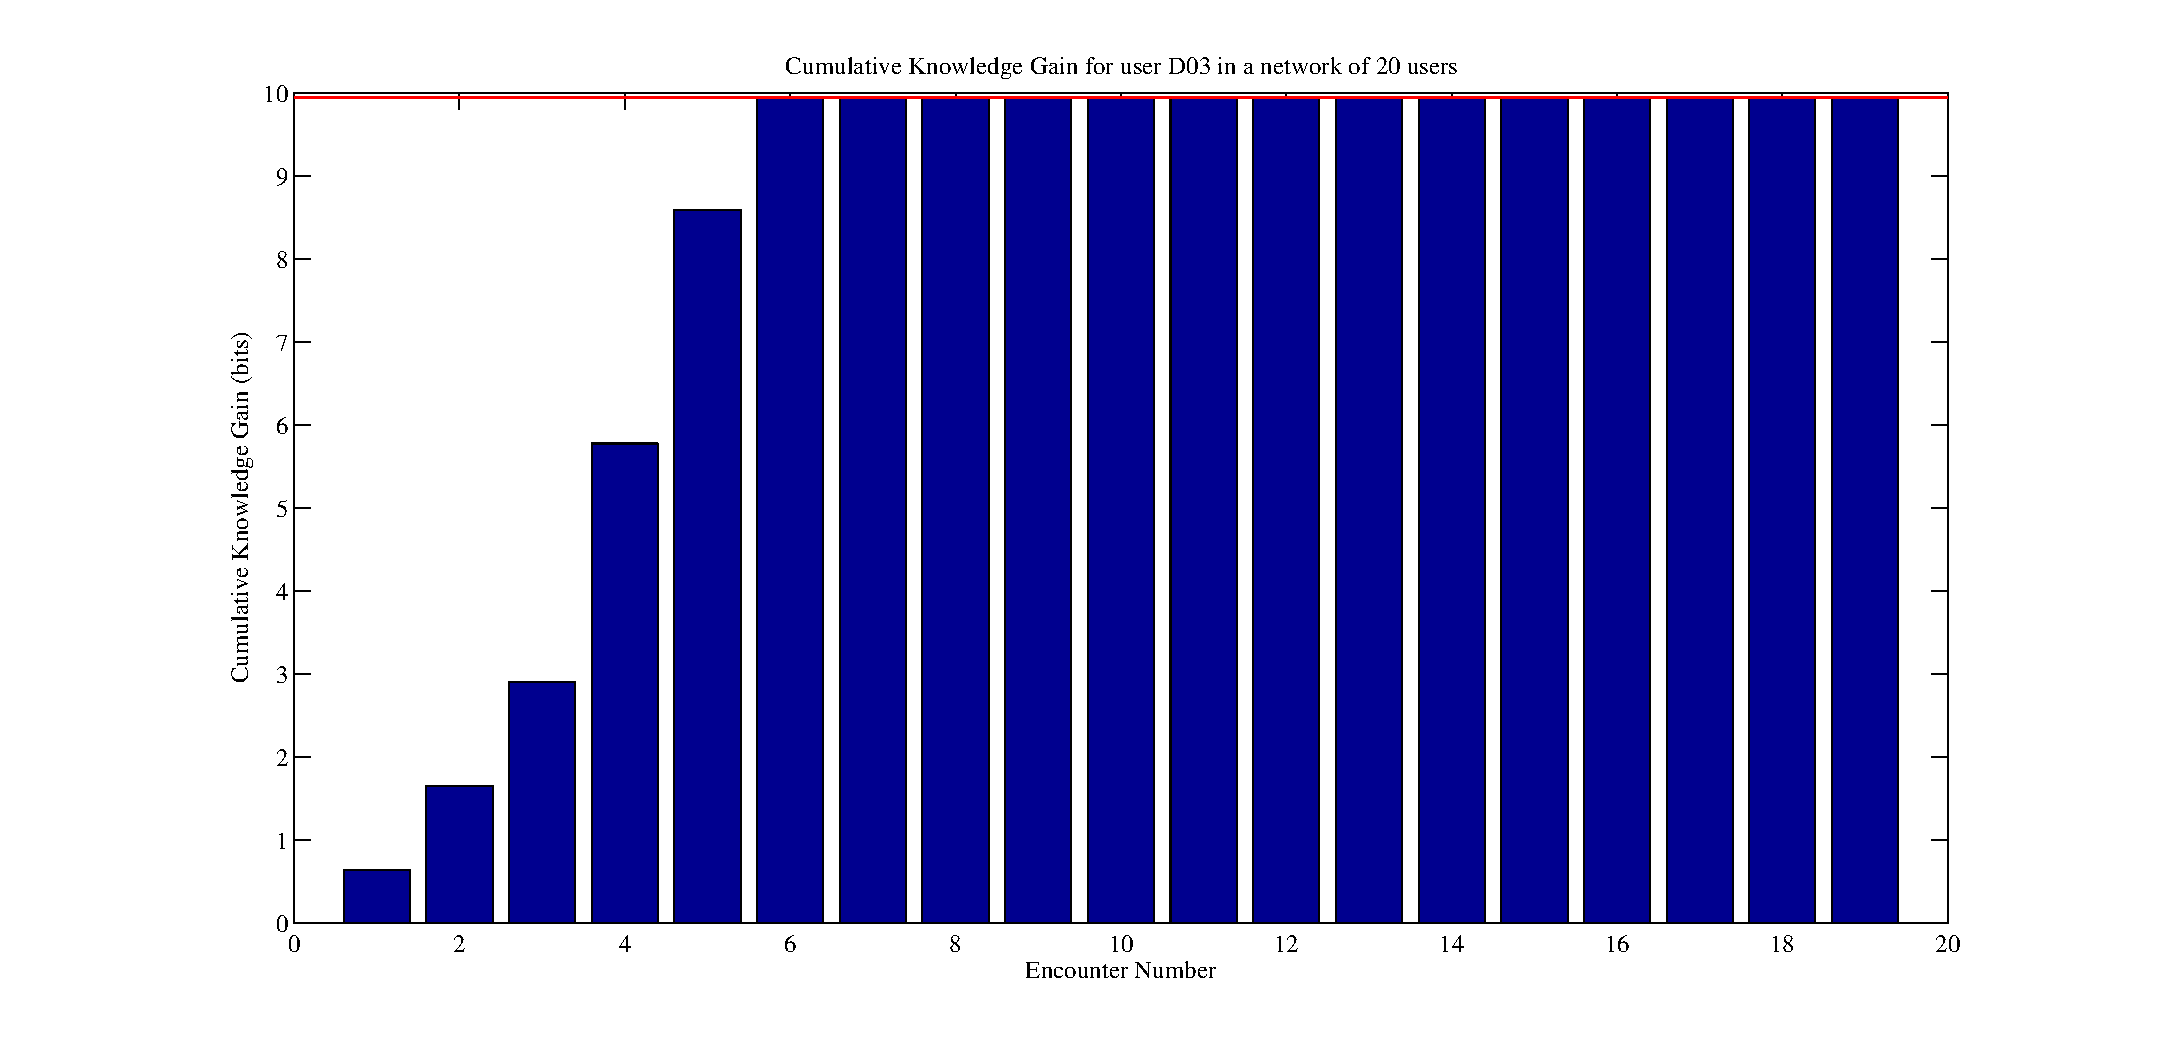
\includegraphics[width=8.1cm ,height=5.6cm]{figures_eps/D03_SSHOP_MO.eps}
%  \centerline{(c)}
    \caption{Cumulative knowledge gain for three users in a single-hop network under FMPO.}\label{fig:B00_SSHOP(MO)}
\end{figure}
%\begin{figure}[!bp]
%\centering
%    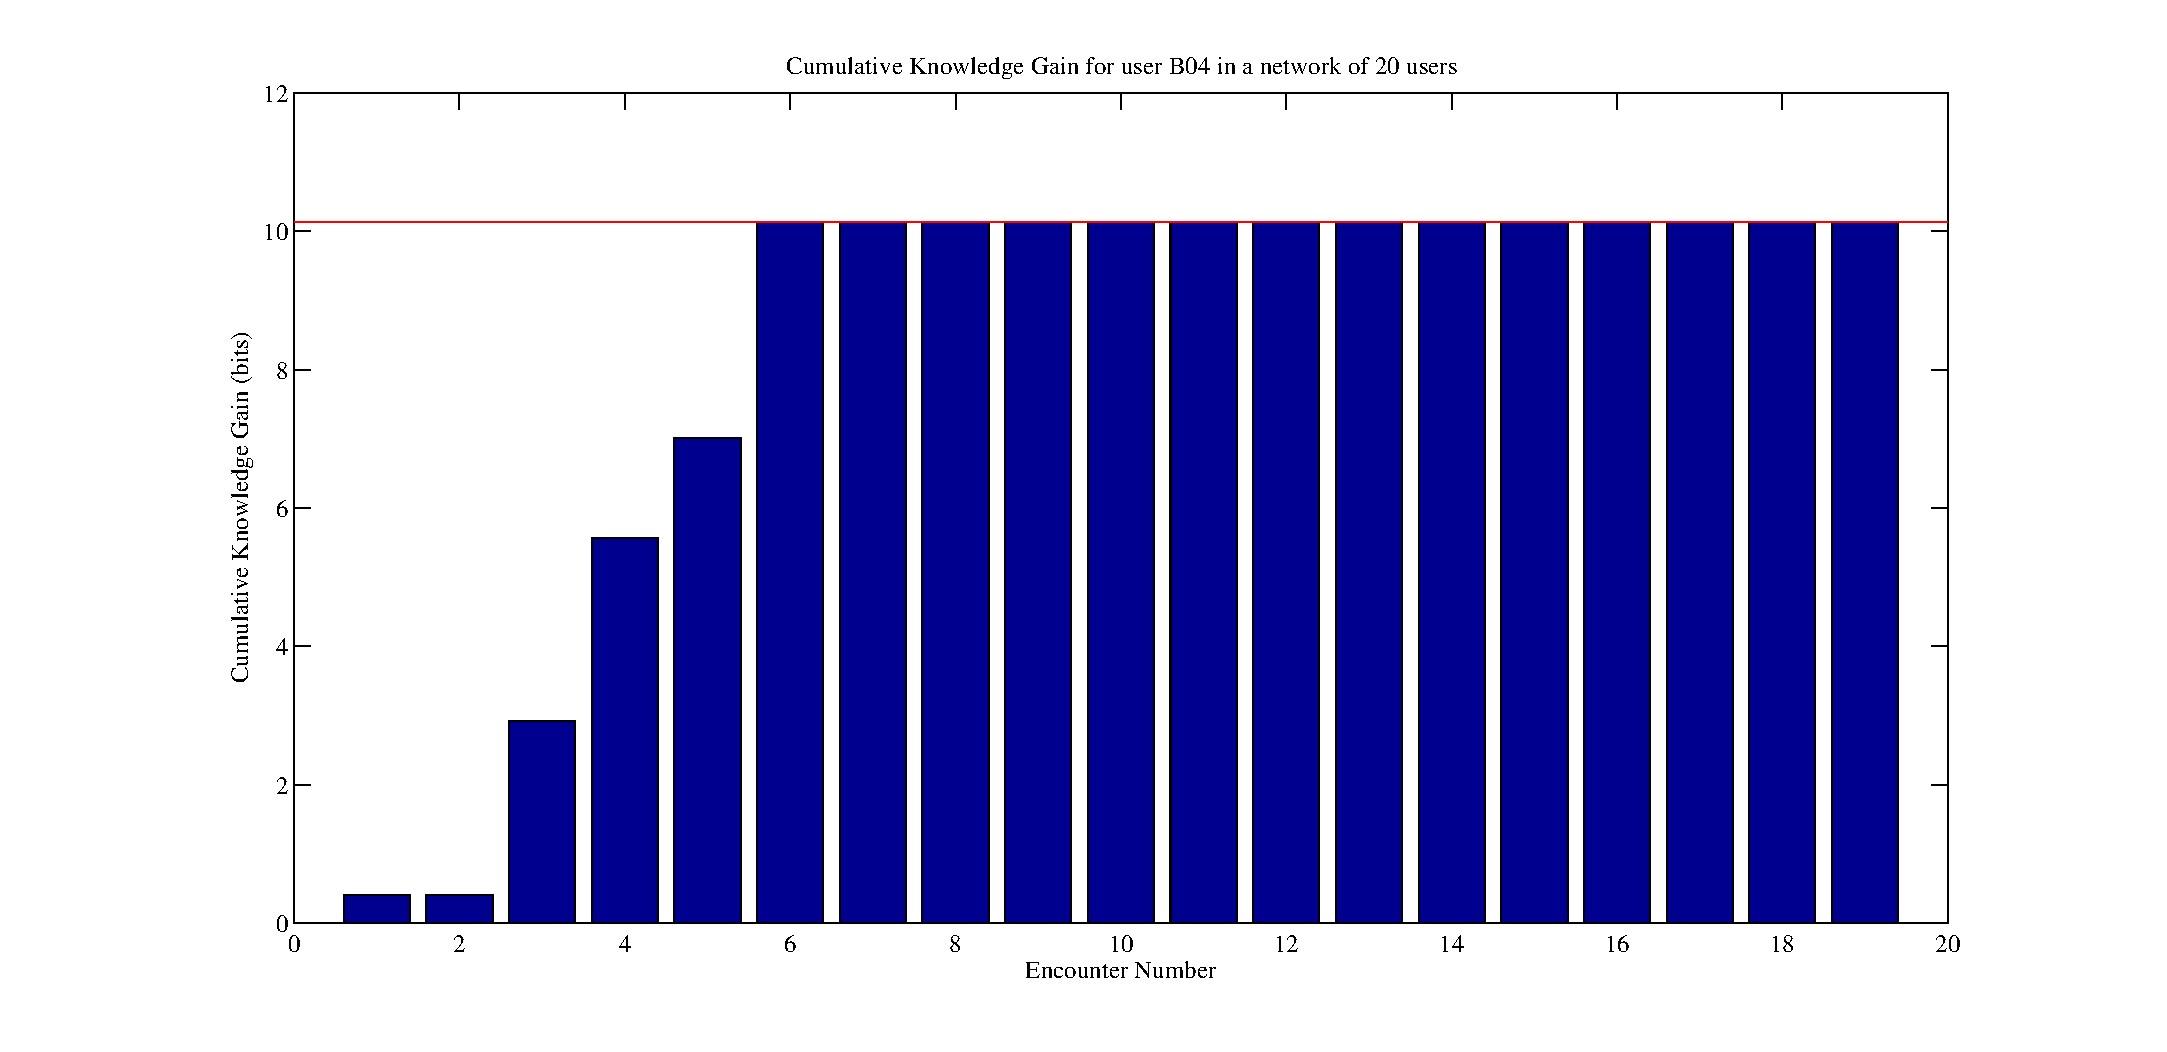
\includegraphics[width=12cm ,height=7cm]{figures_eps/B04_SSHOP_MO.eps}
%    \caption{Cumulative knowledge gain for user B04 in a fixed topology single-hop network under FMPO.}\label{fig:B04_SSHOP(MO))}
%\end{figure}
%    \begin{figure}[!bp]
%\centering
%    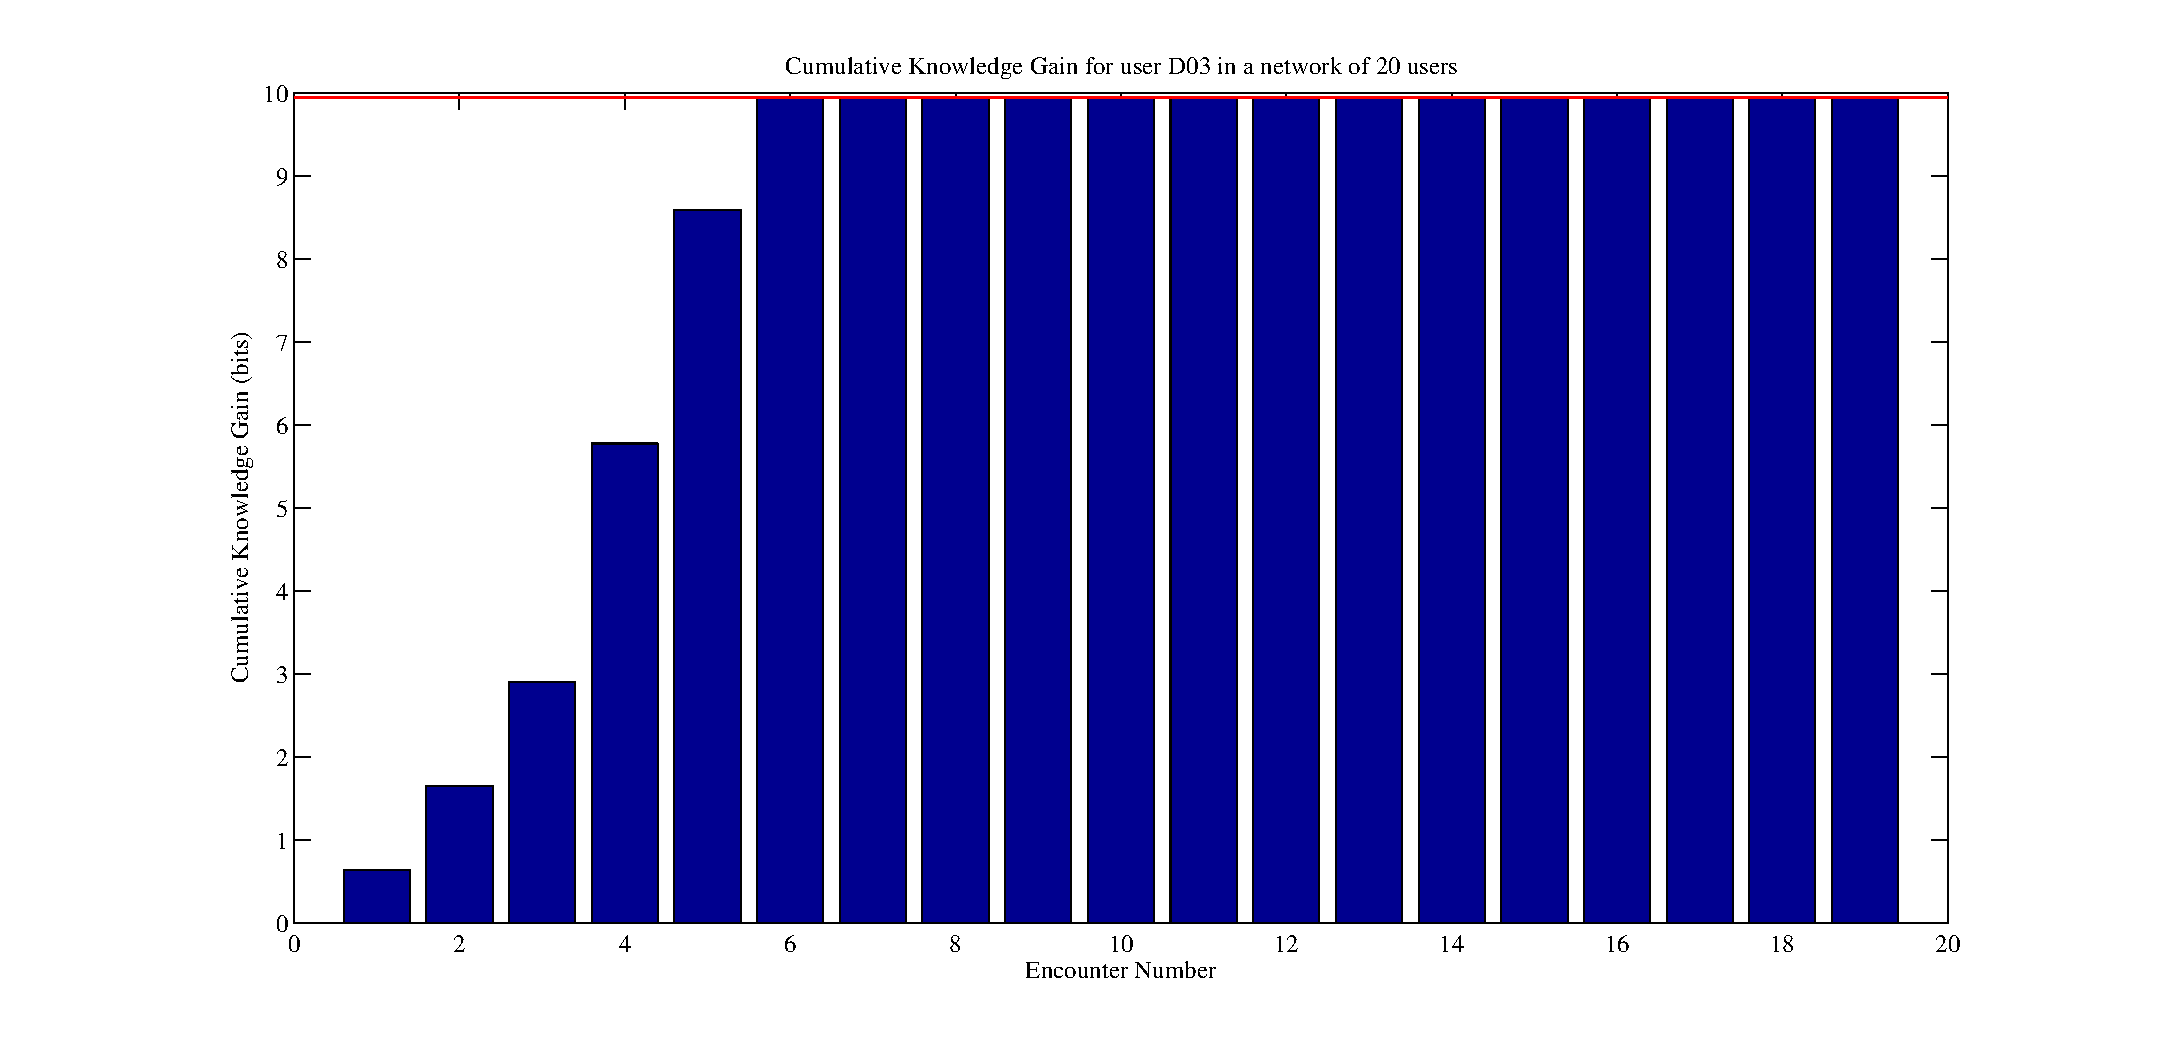
\includegraphics[width=12cm ,height=7cm]{figures_eps/D03_SSHOP_MO.eps}
%    \caption{Cumulative knowledge gain for user D03 in a fixed topology single-hop network under FMPO.}\label{fig:D03_SSHOP(MO))}
%\end{figure}
%=================================================================================================================
%\item Results for Stationary Indirectly Connected (Multi-Hop)- Mine Only Network: 
\vspace{-0.4 cm}
\subsubsection{Fixed Topology, Multi-hop Networks}
%\subsection{Fixed Topology, Multi-hop Similarity-based Networks}
\vspace{-0.2 cm}
%In this section, we shift our attention to fixed topology, multi-hop networks. 
%where we study the cumulative knowledge gain behavior under the SMO and FMPO policies.

As indicated earlier and established in Proposition 4, achieving the KL of an arbitrary user using SMO is fundamentally limited by the single-hop neighborhood size of this node, denoted $N$.
%For this kind of network, any node is limited in achieving the capacity by the neighborhood size. 
To this end, we generate $20$ randomly generated topologies of uniformly distributed users whereby each user has 6-7 single-hop neighbors, out of $20$ nodes, on the average. It can be noticed that $B00$ 
%, namely $B03$, $B05$, $B09$, $B11$, $B07$, $D01$, $D03$, $D05$, 
does not achieve the KL available for it in this network, as established in Proposition 4 and shown here using real smartphone user behavior traces in Fig.~\ref{fig:B00_SMHOP)}. Thus, the maximum KG node $B00$ can achieve is only 43\% of its KL. Similarly, users $B06$ and $D00$ have single-hop neighbors strictly less than $M=20$ and, hence, cannot achieve their respective KLs. 
%This is shown numerically in Fig.~\ref{fig:B00_SMHOP)}.
%
\begin{figure}[!bp]
\centering
 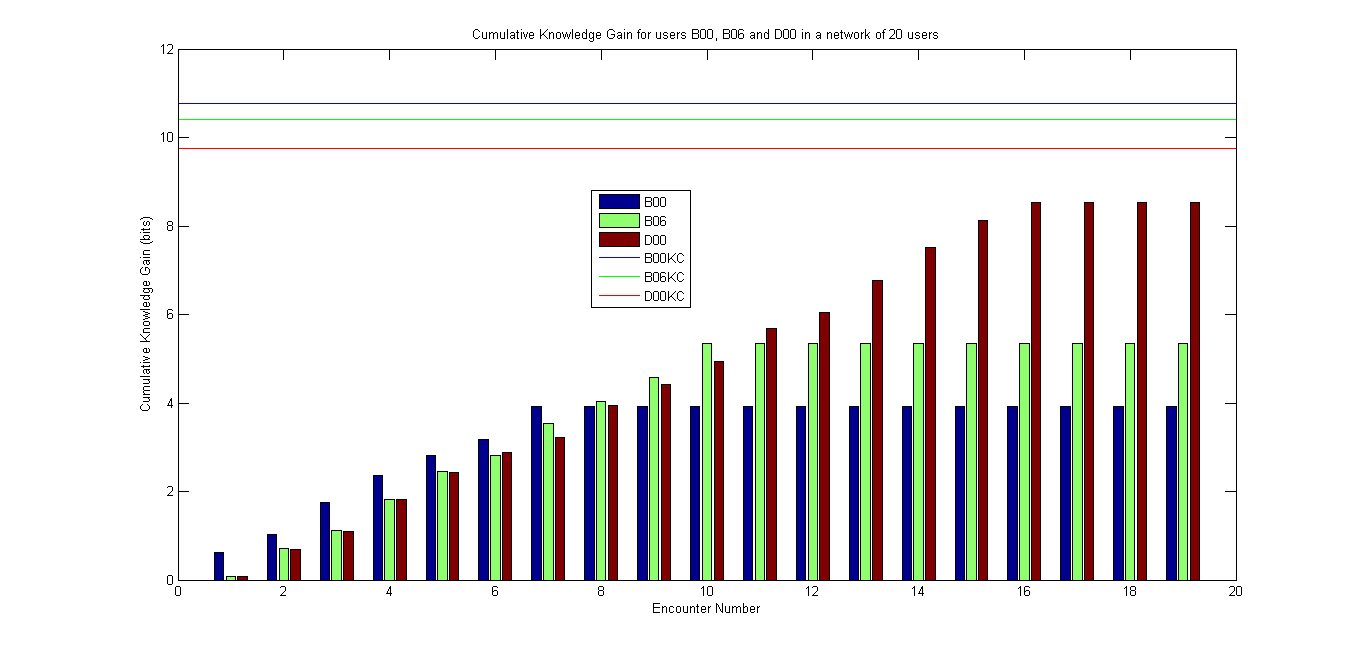
\includegraphics[width=10cm ,height=5.6cm]{figures_png/Fig7}
% 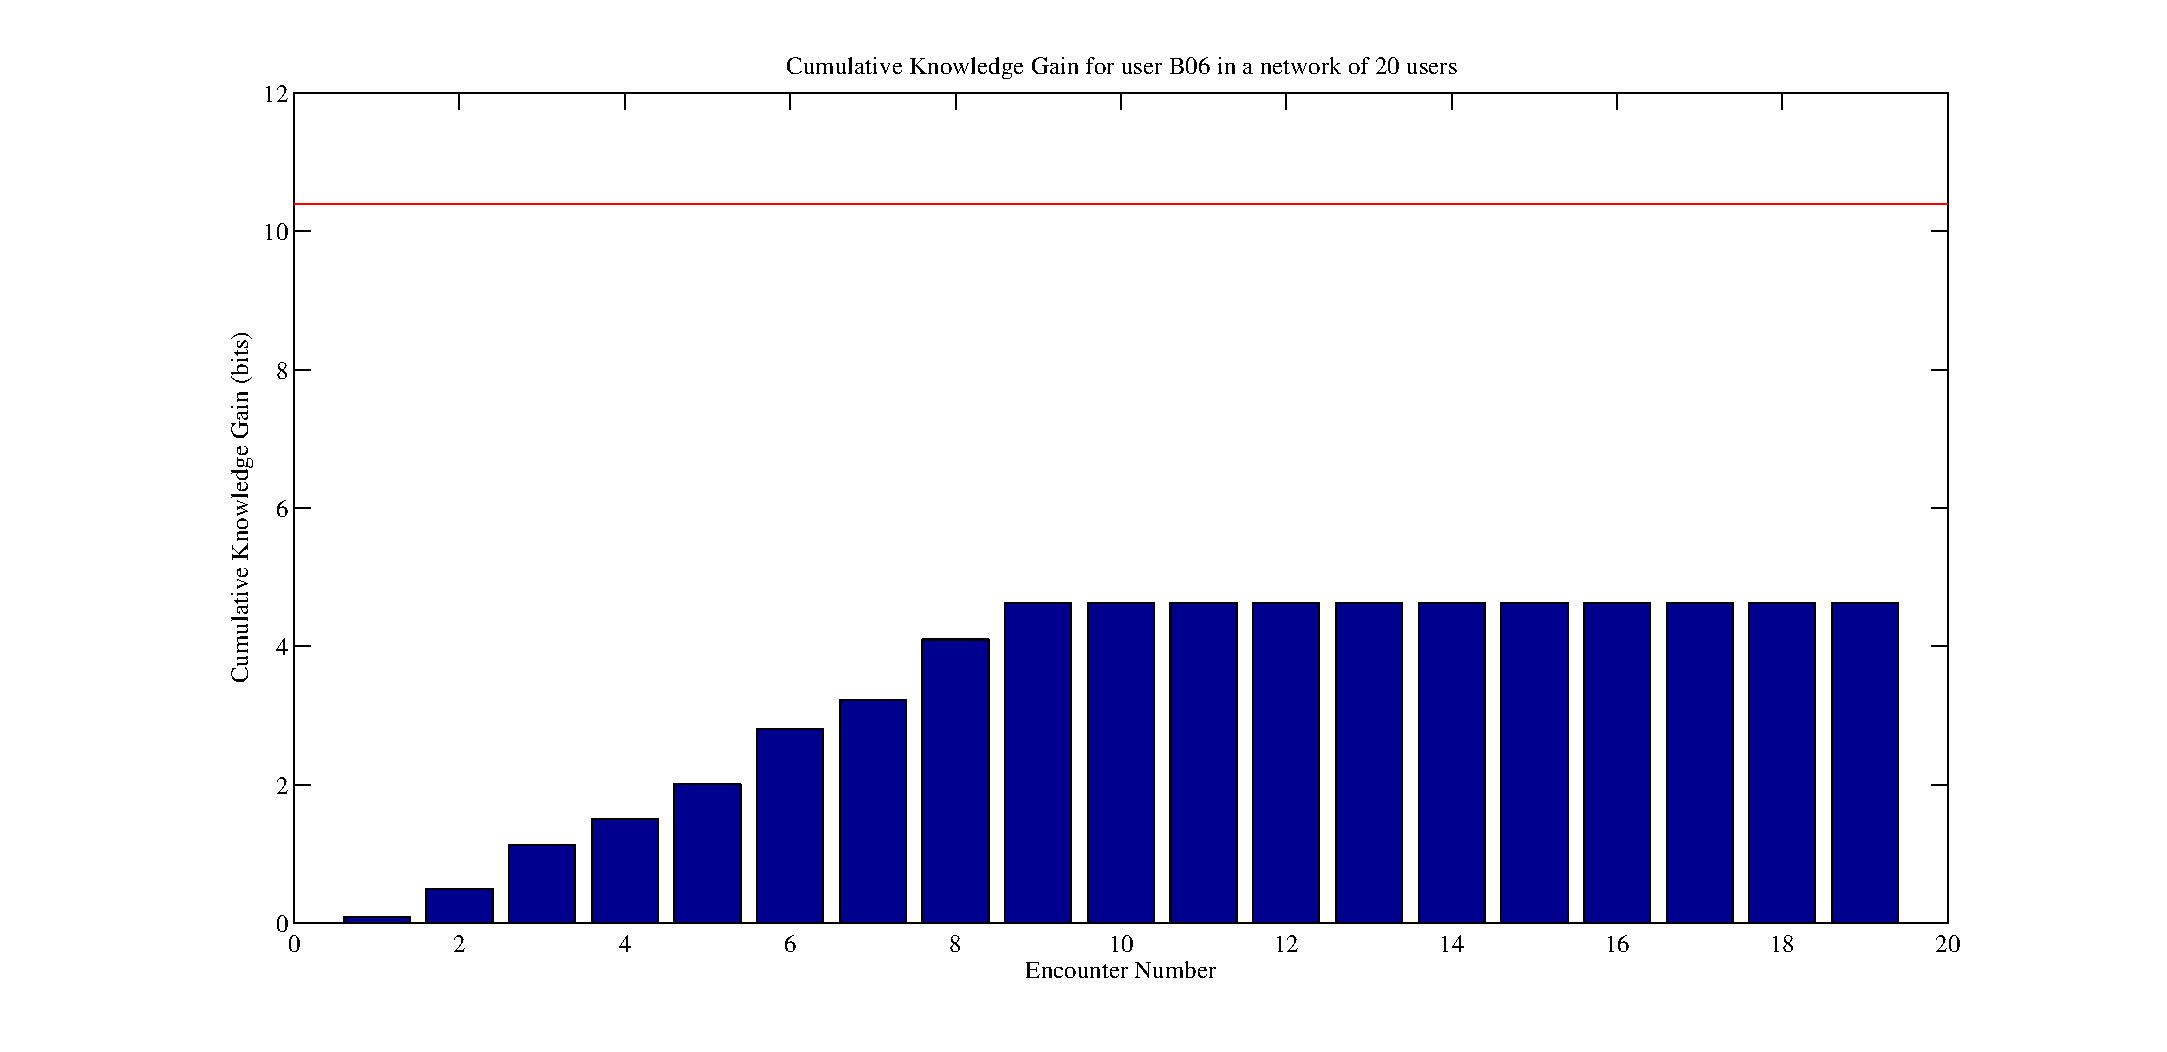
\includegraphics[width=8.1cm ,height=5.6cm]{figures_eps/B06_SMHOP}
% \centerline{(a) \hspace{9 cm} (b)}
% 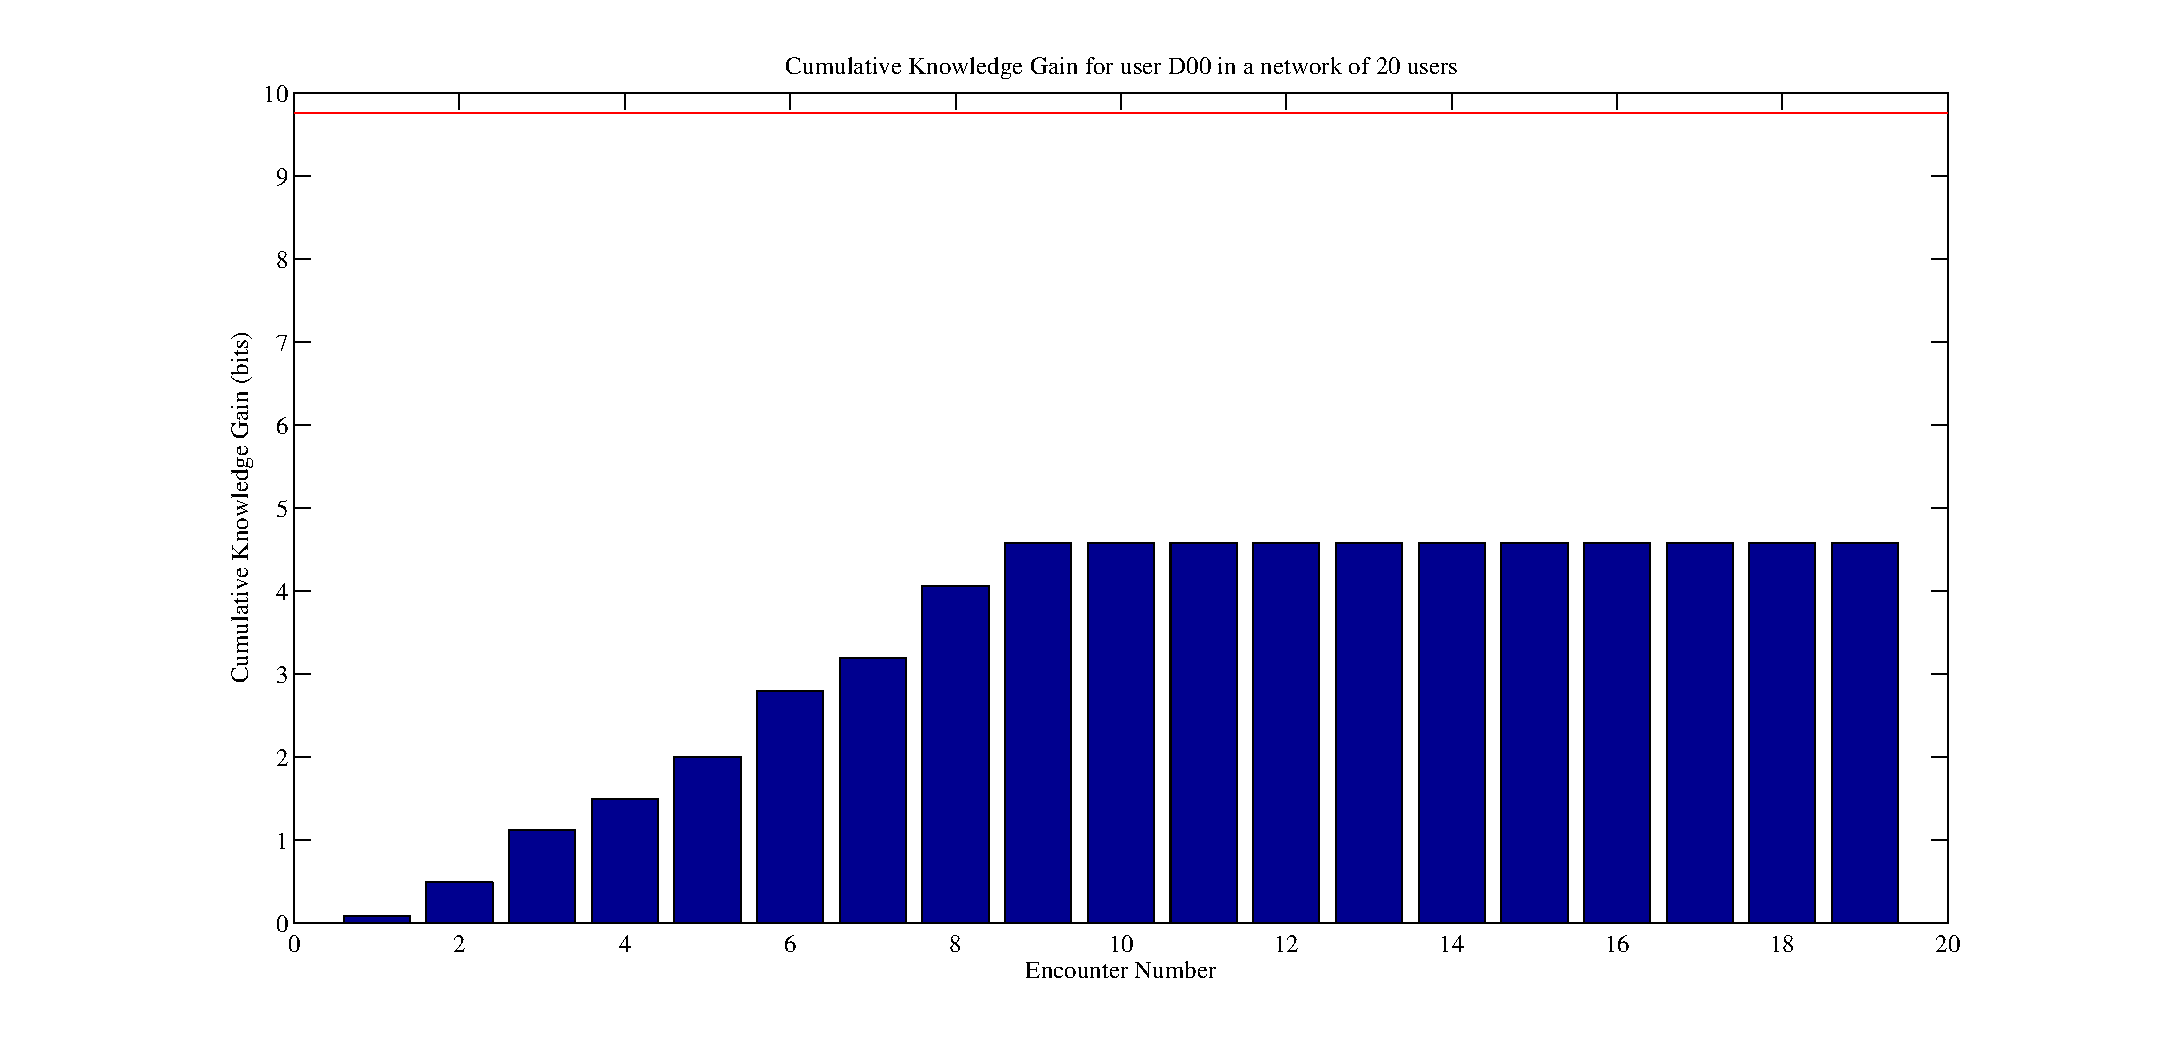
\includegraphics[width=8.1cm ,height=5.6cm]{figures_eps/D00_SMHOP}
% \centerline{(c)}
    \caption{Cumulative knowledge gain for three users in a fixed multi-hop network under SMO.}\label{fig:B00_SMHOP)}
\end{figure} 
%\begin{figure}[!bp]
%	\centering
%     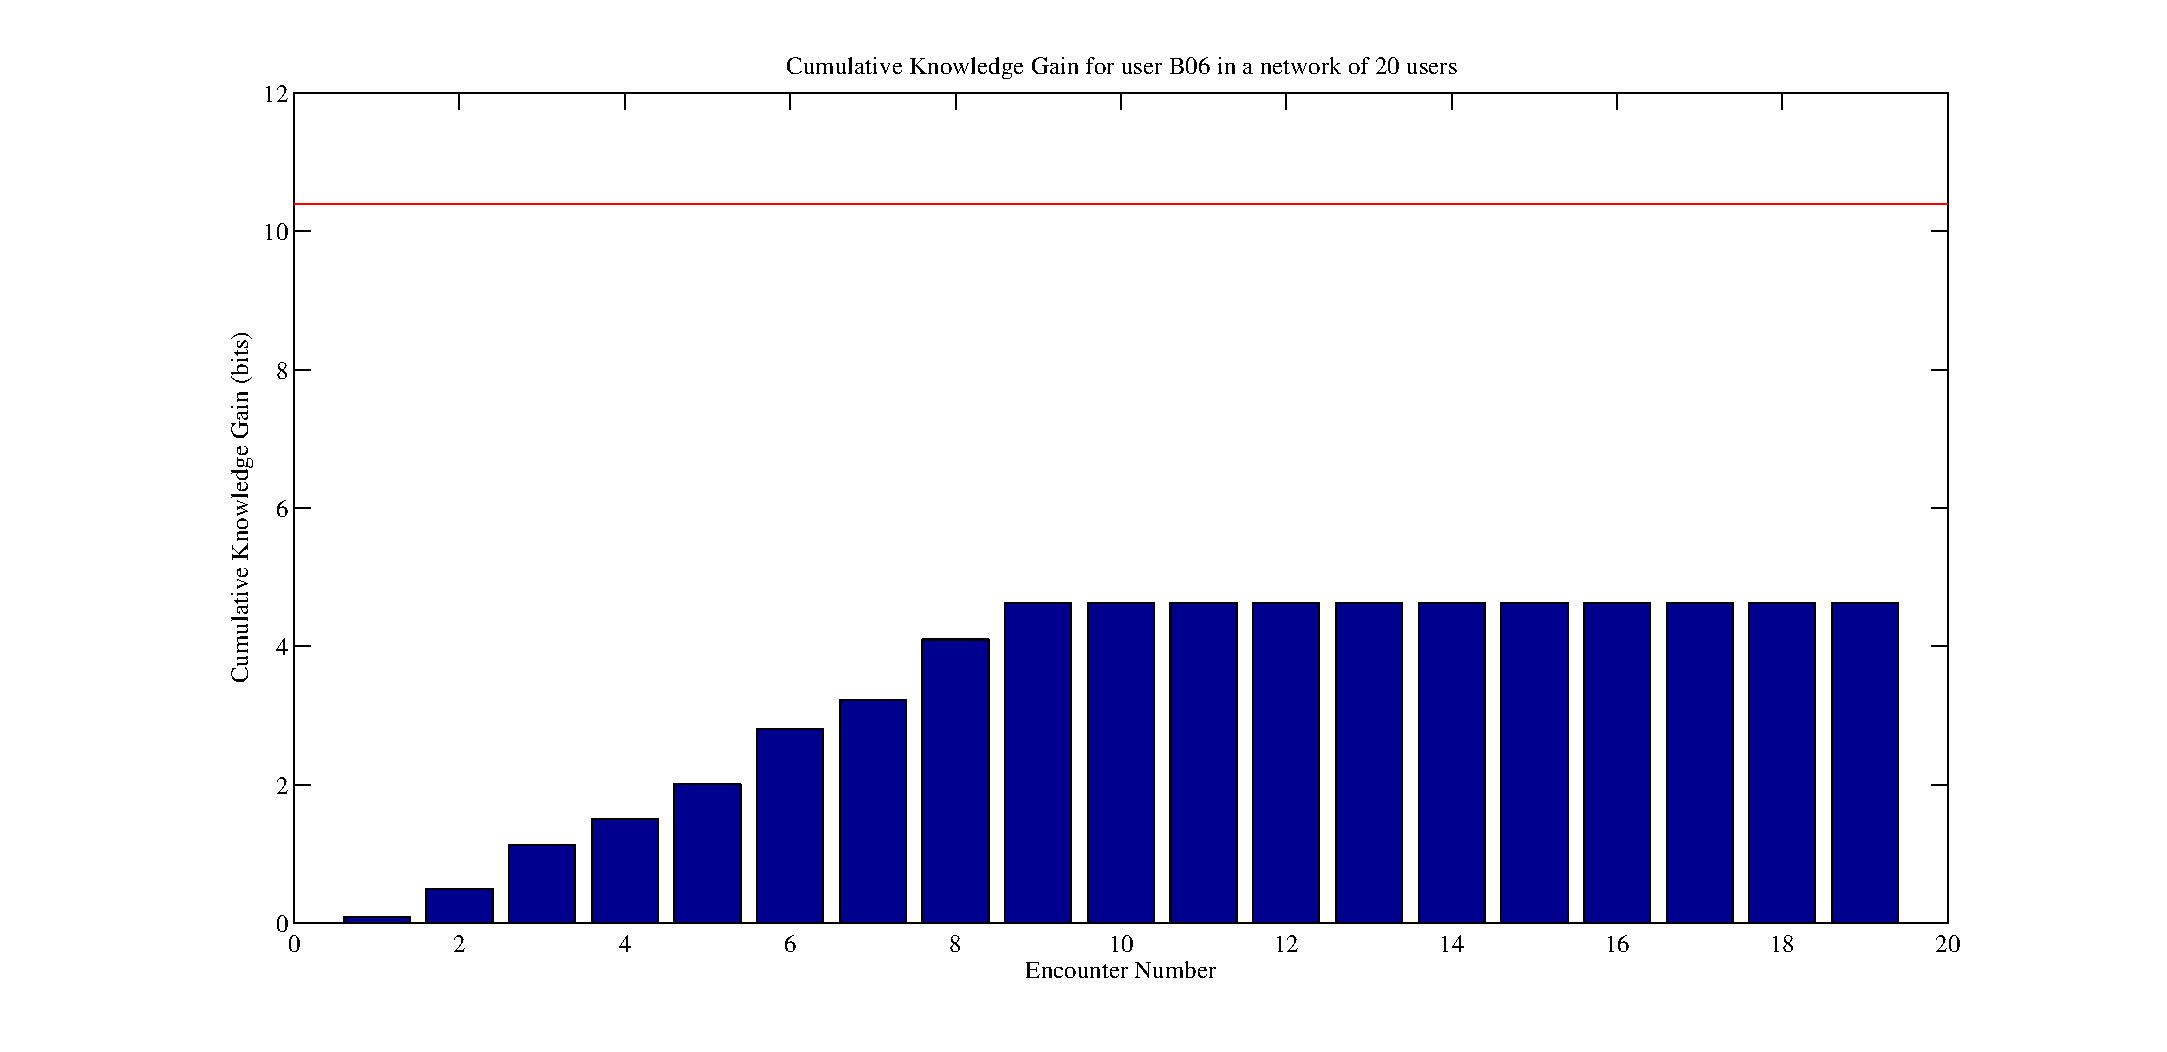
\includegraphics[width=12cm ,height=7cm]{figures_eps/B06_SMHOP}
%    \caption{Cumulative knowledge gain for user B06 in a fixed topology multi-hop network under SMO.}\label{fig:B06_SMHOP)}
%\end{figure}
%\begin{figure}[!bp]
%	\centering
%     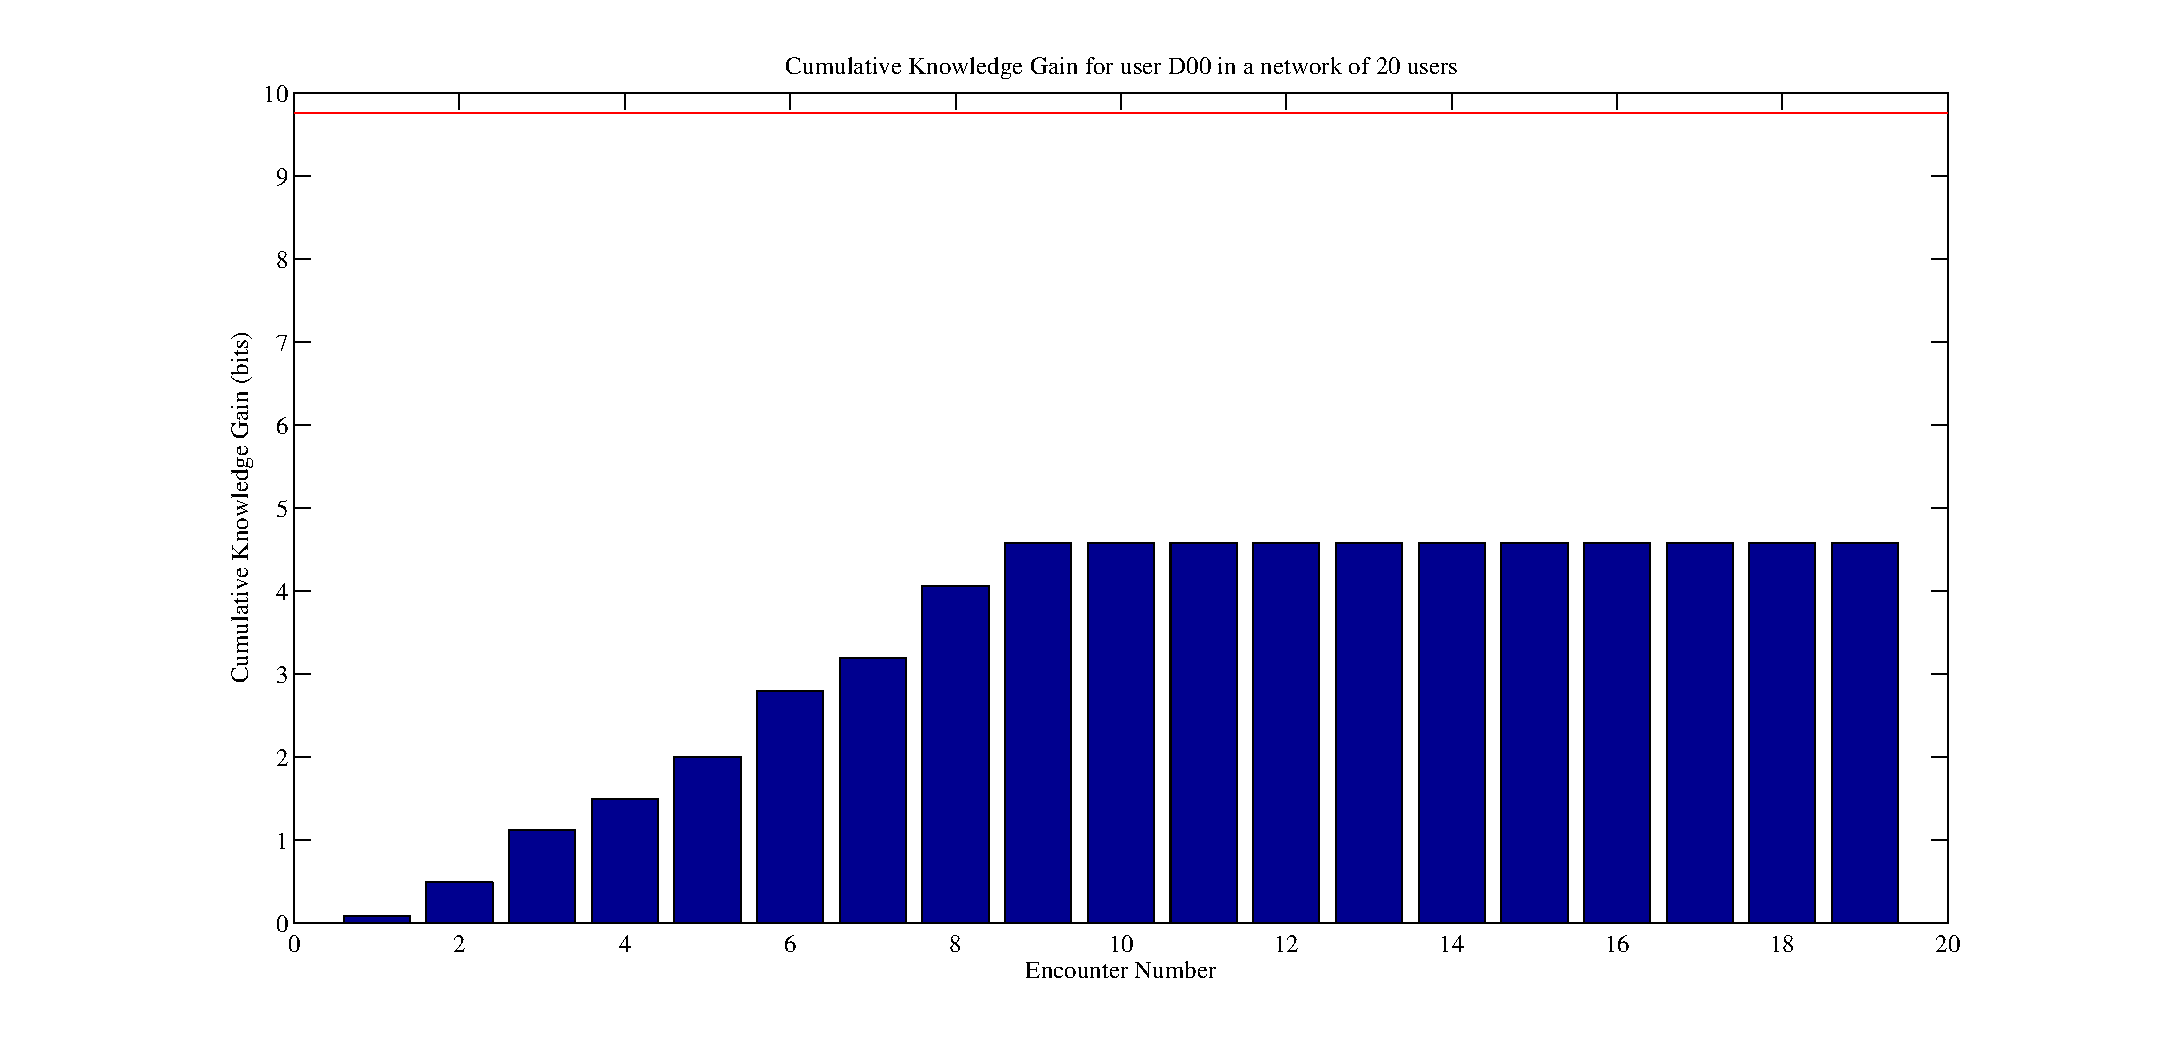
\includegraphics[width=12cm ,height=7cm]{figures_eps/D00_SMHOP}
%    \caption{Cumulative knowledge gain for user D00 in a fixed topology multi-hop network under SMO.}\label{fig:D00_SMHOP)}
%\end{figure}
    
%\item Results for Stationary Indirectly Connected (Multi-Hop)- Mine Plus Others' Network: 
Finally, we analyze the KG and KL performance of the FMPO policy in multi-hop topologies. In this case, the FMPO policy is expected to overcome the limited neighborhood problem due to sharing others' knowledge (tips) and, hence, the nodes could achieve the knowledge limit as shown in Proposition 5. The results here are based on $20$ randomly generated topologies.  
%The first layer contains node $B00$, the second layer contains ten nodes and the third layer contains nine nodes. 
%It is assumed that a node in one tier could only encounter nodes in the directly lower or higher tier. 
The cumulative knowledge gains for users $B00$, $B06$ and $D00$ are depicted in Fig.~\ref{fig:B00_SMHOP_MO)}. We notice that the KL is achievable for the three shown users after $8$, $9$ and $10$ encounters, respectively.
%
  \begin{figure}[!bp]
	\centering
     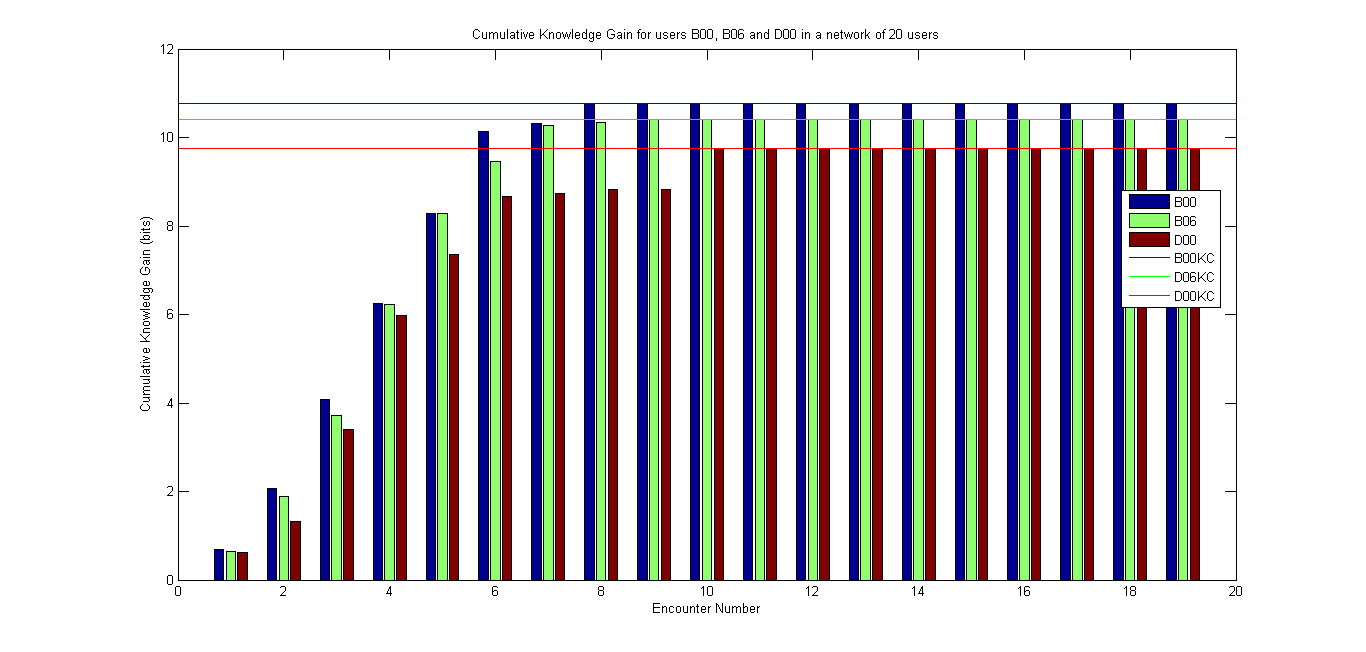
\includegraphics[width=10cm ,height=5.6cm]{figures_png/Fig8}
%     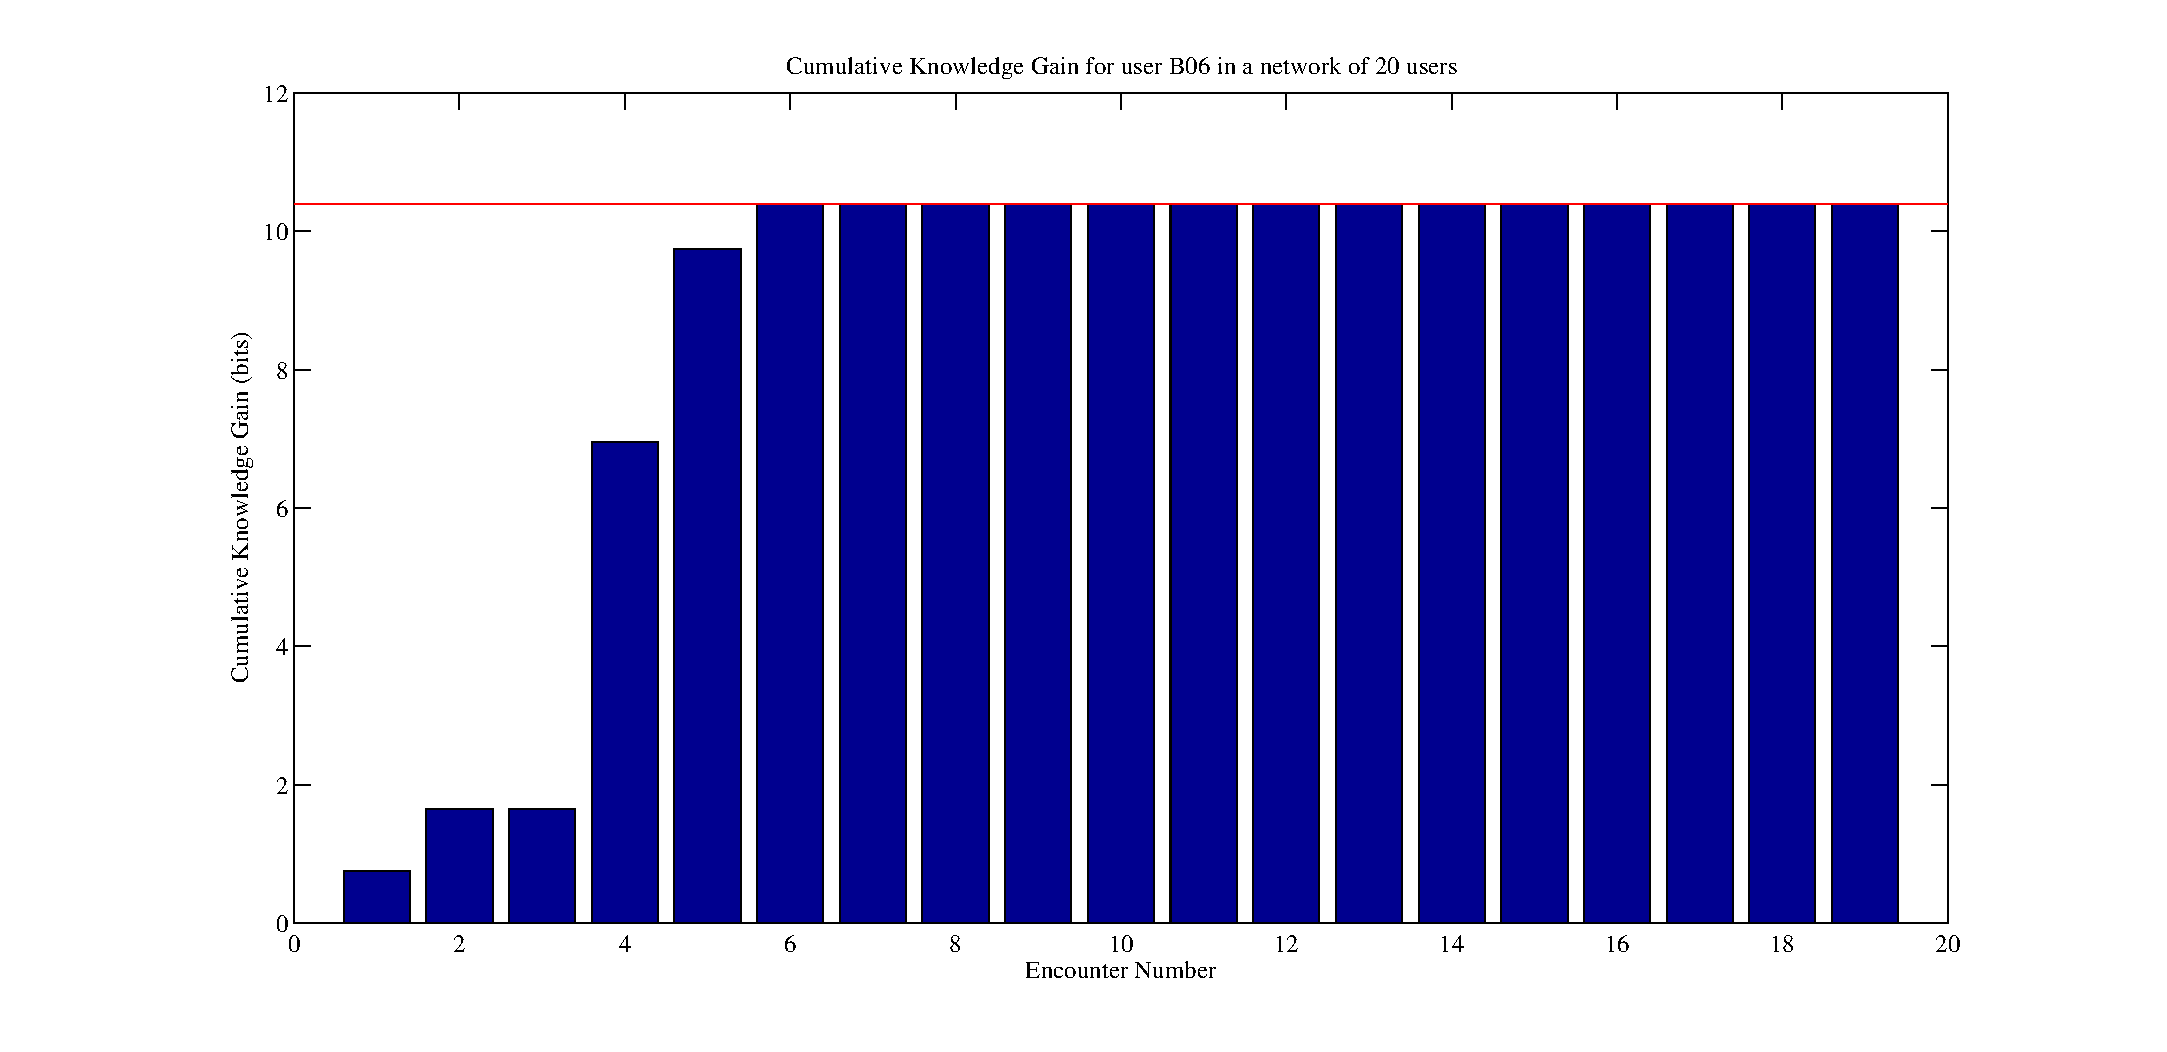
\includegraphics[width=8.1cm ,height=5.6cm]{figures_eps/B06_SMHOP_MO}
% \centerline{(a) \hspace{9 cm} (b)}
%     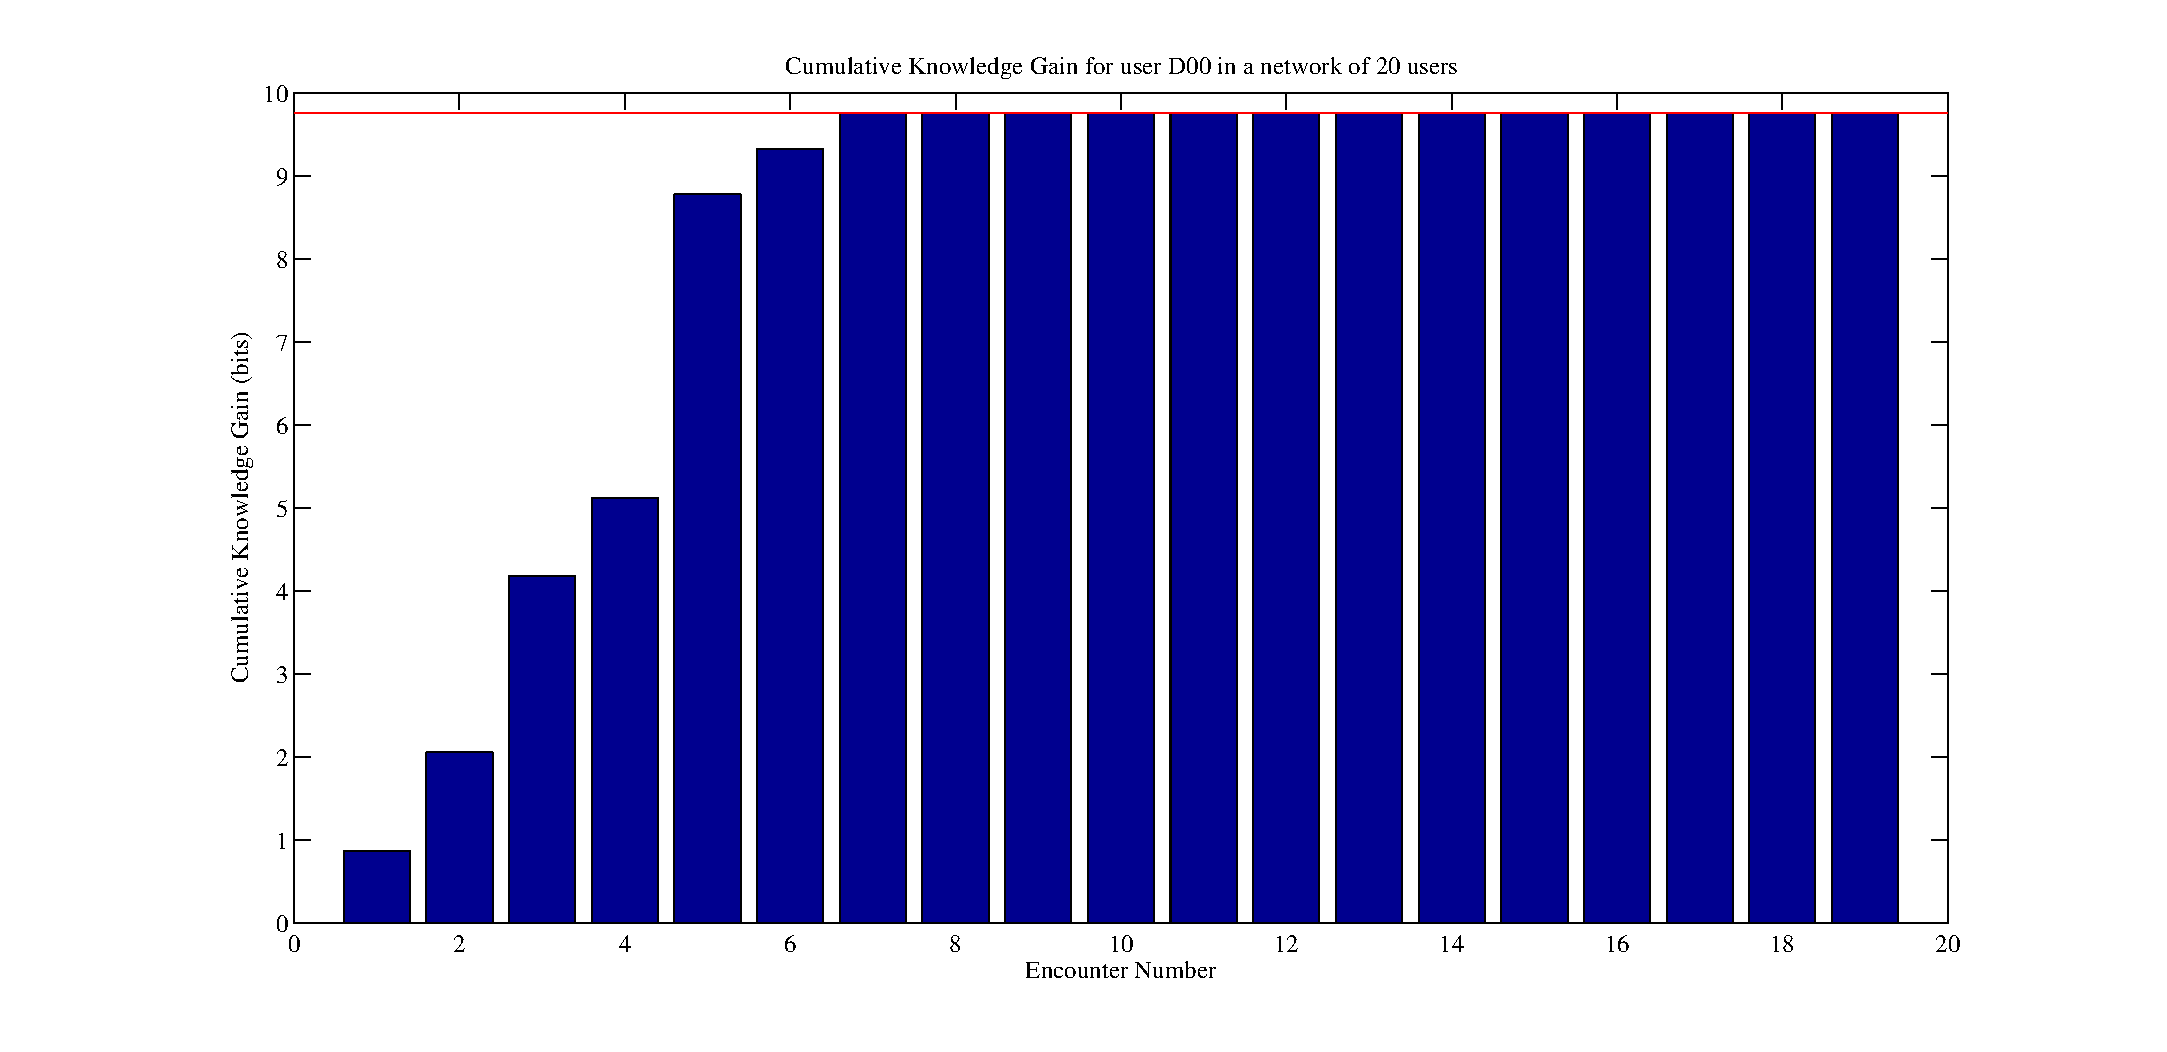
\includegraphics[width=8.1cm ,height=5.6cm]{figures_eps/D00_SMHOP_MO}
%     \centerline{(c)}
    \caption{Cumulative knowledge gain for three users in a fixed multi-hop network under FMPO.}\label{fig:B00_SMHOP_MO)}
\end{figure}
%\begin{figure}[!bp]
%	\centering
%     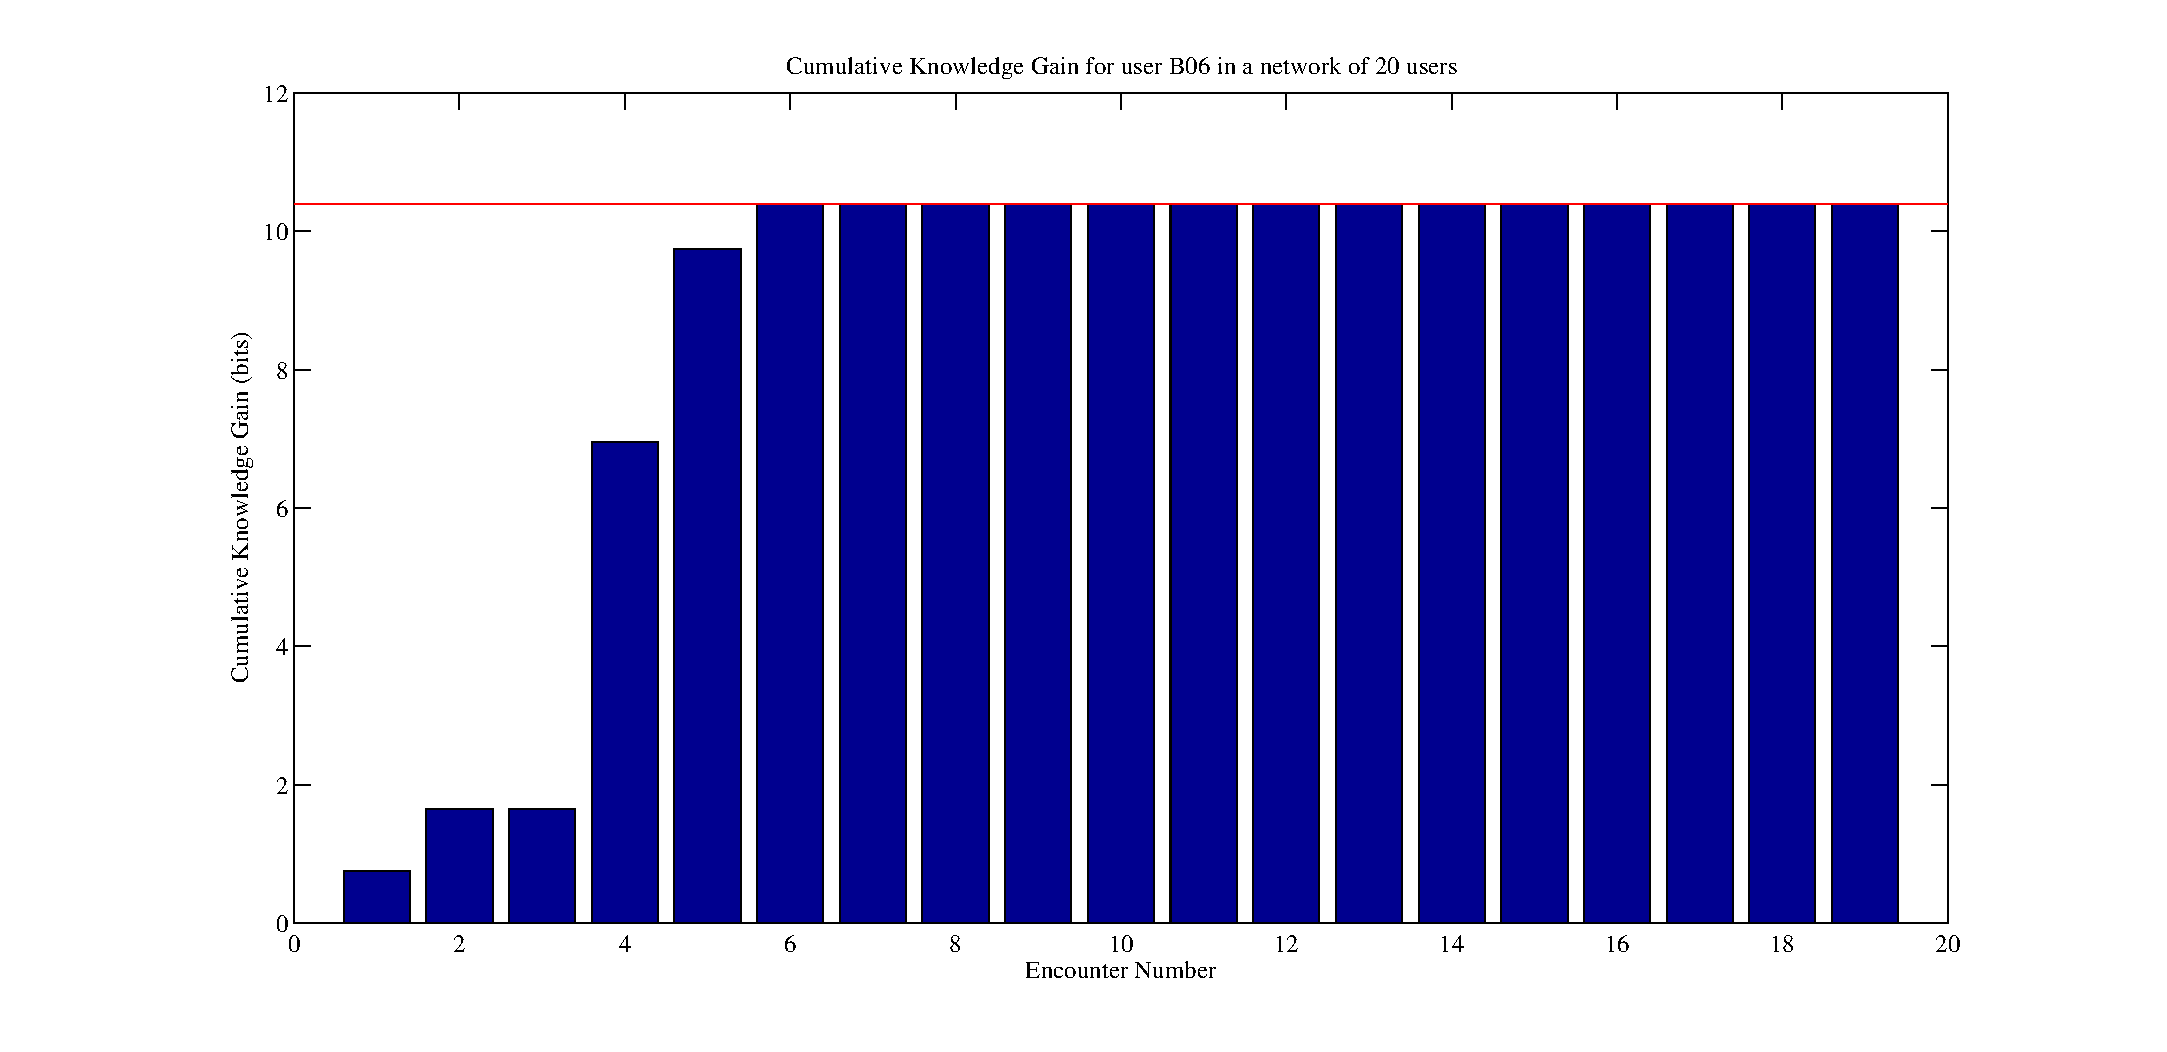
\includegraphics[width=12cm ,height=7cm]{figures_eps/B06_SMHOP_MO}
%    \caption{Cumulative knowledge gain for user B06 in a fixed topology multi-hop network under FMPO.}\label{fig:B06_SMHOP_MO)}
%\end{figure}  
%\begin{figure}[!bp]
%	\centering
%     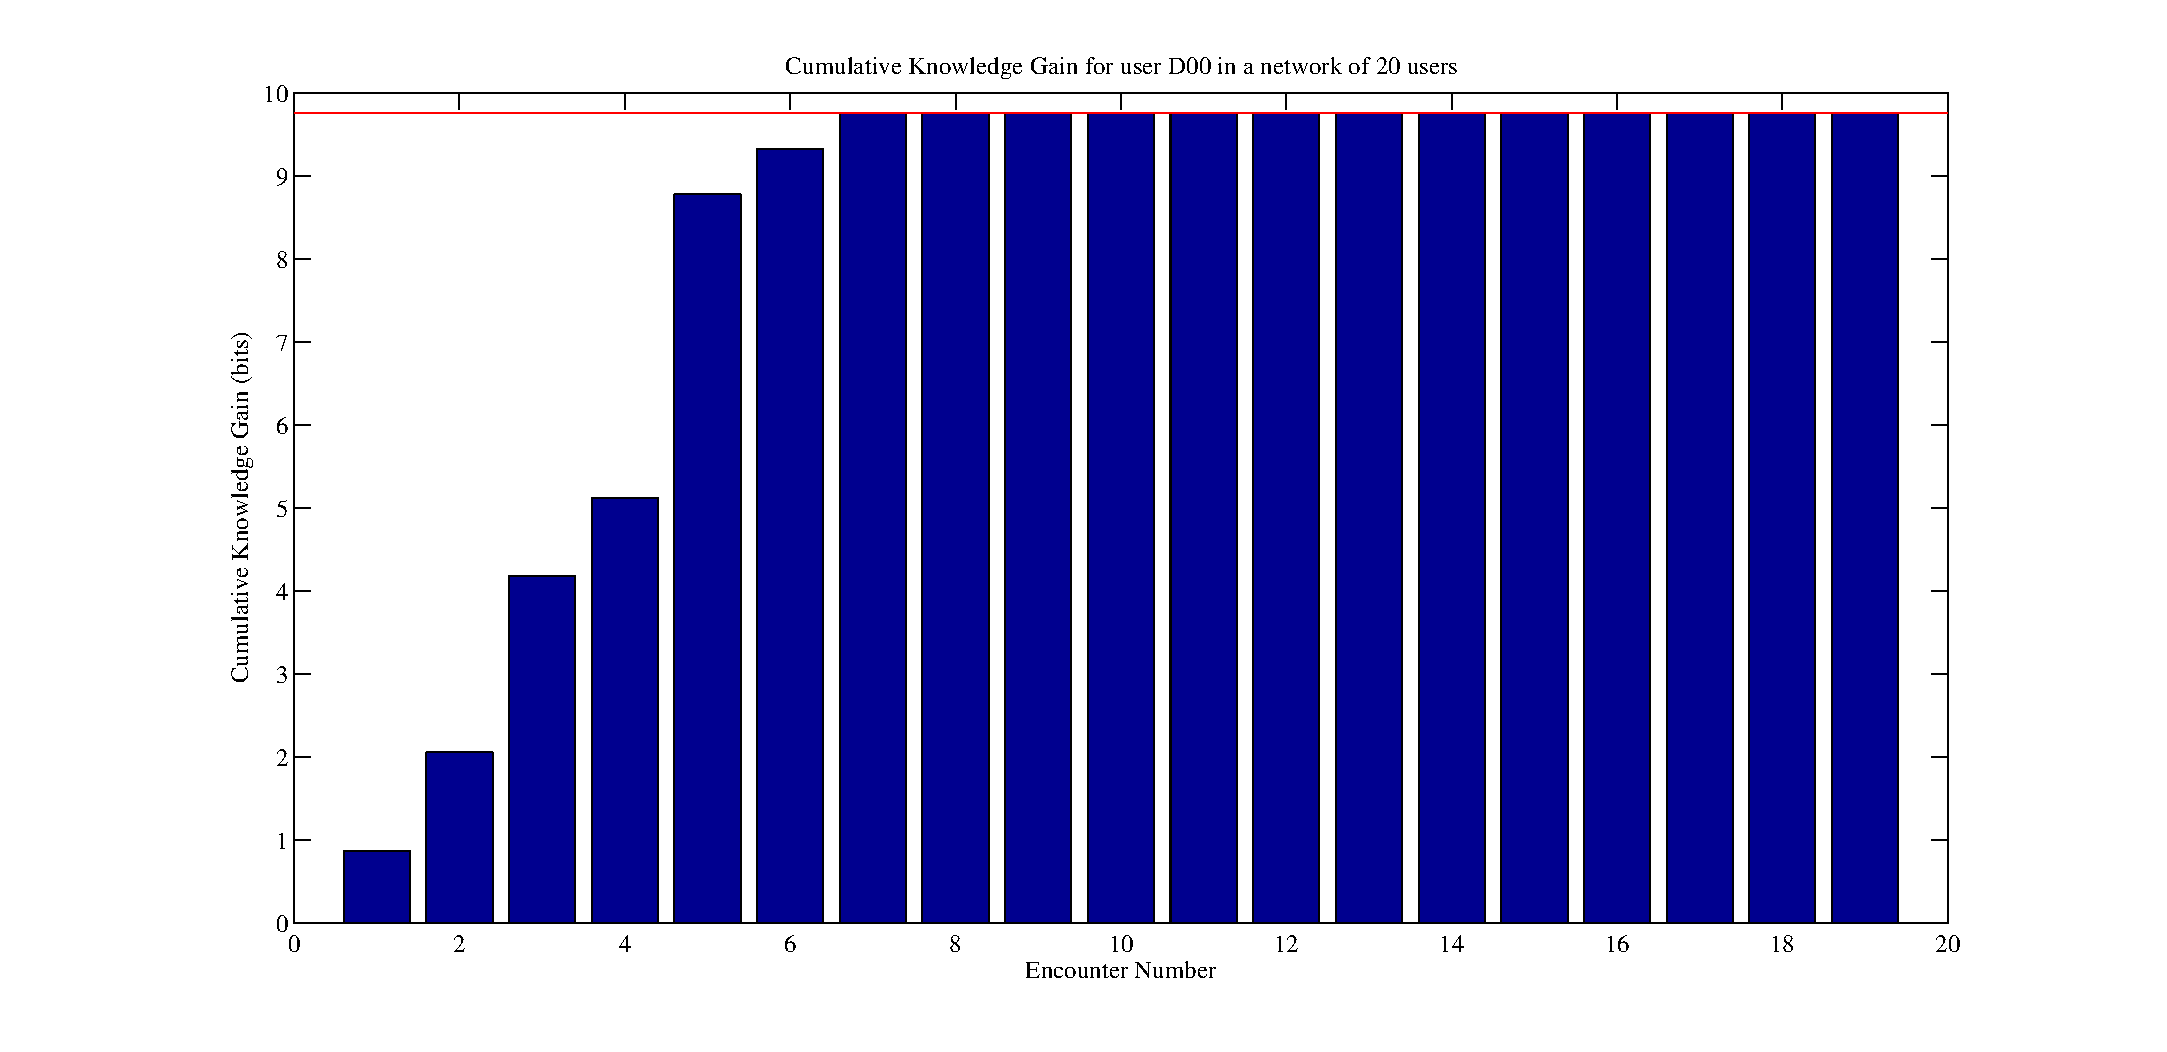
\includegraphics[width=12cm ,height=7cm]{figures_eps/D00_SMHOP_MO}
%    \caption{Cumulative knowledge gain for user D00 in a fixed topology multi-hop network under FMPO.}\label{fig:D00_SMHOP_MO)}
%\end{figure}
%
%\end{itemize}
%==================================================================================================
\vspace{-0.6 cm}
\subsubsection{Time-varying Topology (Mobile) Networks}
%\subsection{Time-varying Topology (Mobile) Similarity-based Networks}
\vspace{-0.2 cm}
%\subsubsection{User Profile and Mobility Traces}
%
\noindent {\it A. User Profiles and Mobility Traces}\\
%\subsubsection{User Profile and Mobility Traces}
%
After an extensive search for mobile user traces on publicly available data repositories, e.g., CRAWDAD \cite{infocom,diot} and the alike, we did not find traces that include both, user behavior and mobility traces. Moreover, most of the mobility traces are university campus Wi-Fi access patterns as opposed to mobile user encounters. In order to proceed with the performance evaluation based on real data, we resort to jointly leveraging traces from two
different data sets, for user behavior and mobility. First, user profiles are constructed based on the LiveLab project data \cite{data} described earlier. On the other hand, mobility traces are based on a ``conference encounter'' data, namely Infocom 2005 \cite{infocom,diot}. 
%Towards this objective, we jointly leverage the user profile probability distributions, constructed from the LiveLab data, along with the Infocom user mobility traces. 
For the Infocom 2005 experiment, the data set is relatively small whereby participants are $50$ attending the student workshop. Nevertheless, it constitutes a reasonably sized set for our performance evaluation purposes. The students were given iMotes on March $7^{th}$, $2005$ between lunch time and $5$ pm and collected on March 10th, 2005 in the afternoon. Two iMotes were lost while seven did not deliver useful data due to an accidental hardware reset. Contacts with these nine iMotes were discarded from the traces of others to avoid any effect on the results. 
The first six hours are discarded since they were attending the same workshop. We consider the contacts of $20$ nodes only to match the number used from the LiveLab user profiles data. Thus, we associate the profiles of $20$ randomly chosen users from the LiveLab data set 
%$B00$, $B02$, $B03$, $B04$, $B05$, $B06$, $B07$, $B08$, $B09$, $B10$, $B11$, $D00$, $D01$, $D02$, $D03$, $D04$, $D05$, $D06$, $D07$ and $D08$ 
to the mobility traces of $20$ iMotes from Infocom 2005 and monitor them for half a day. This enables us to conduct our knowledge sharing analysis and collect the sought performance results.
%quantify the cumulative knowledge gain after each encounter and whether the gain will reach capacity or not and how many encounters would it take until achieving capacity.

Despite the fact that user profile and mobility traces are brought from two totally independent data sets, we find it a very useful attempt towards evaluating our policies, due to the lack of the sought data in the public domain. This constitutes a strong motivation for the mobile networking and computing community to focus on the social dimension as well as the mobility and wireless connectivity dimensions, which already have several data sets in the public domain.
%
%For mobile similarity-based opportunistic networks and modeling the user as a Random Variable, 
%we will be conducting our experiments using LiveLab data \cite{data} described earlier and InfoCom 2005 mobility traces. We project the PMFs from LiveLab data onto the user mobility traces \cite{infocom} from the conference IEEE Infocom 2005. 
%
%==================================================================================================
%\subsubsection{Mobile directly Connected (Single Hop) Network:}
%
%\noindent {\it B. Mobile, Single-hop Networks}\\
%Despite the fact that this is a mobile network, it is easy to notice 
%that it is not much different from fixed topology networks, since nodes remain one-hop away from each other all the time, in both cases.

%If we think thoroughly about this kind of network, we will find that all nodes in the network are one hop away from each other. Even when the nodes move, they are still in each other's range. 
%Accordingly, nodes' mobility in this case does not have an effect on the KG and KL at all. 
%Each time a node wants to exchange information with other nodes, he/she will poll to see what nodes are in its range and the result will be that all nodes are in its range. 
%This is the same case of the Stationary directly Connected (Single Hop) Network with its two cases; Forward Mine Only and Forward Mine Plus Others'. So, the same results will be achieved as in the last section.\\ 
%=================================================================================================
%
%\subsubsection{ Mobile Indirectly Connected (Multi Hop) Network:}
\vspace{0.1 cm}
\noindent {\it B. Performance Results}\\
%\subsubsection{Time-varying Topology, Multi-hop Networks}
In this section, we quantify the knowledge limit and gain of time-varying topology (mobile) multi-hop networks, under the two sharing policies. 
%Recall that the case of mobile, single-hop networks simply reduces to fixed topology, single-hop networks studied in Section 3.3.1.A.
Intuitively, users' mobility would play a key role in whether a node can achieve its 
KL and, if so, how much time this would incur. 
%We evaluate the KG and KL performance for the SMO and FMPO policies, using the LiveLab profile traces and Infocom 2005 mobility traces.
%
%As a result, Mobility is a factor in achieving/not achieving knowledge capacity and how fast a node could achieve this capacity. 
%We investigate this kind of network for the two cases; Mine Only and Mine Plus Others' using Infocom traces. 
%
The gathered results are shown in Table ~\ref{tab:Infocom}. We compare the KG acquired by 
sample nodes using SMO in two cases, namely the stationary case where a snapshot is taken at time $t=0$ and the mobile case over half a day. At time $t=0$, 
all nodes, except for node $B07$, are disconnected yielding KG of zero. Node $B07$ is initially connected to $D06$ and reaps a KG of 0.64 as shown. The intriguing observation here is that mobility does help some nodes to approach the knowledge limit. On the other hand, some nodes, e.g., $B06$, do not benefit from mobility since they remain disconnected throughout the 
experiment lifetime. This insight agrees with intuition since the mobility patterns of some nodes could assist them in encountering the ``knowledge hot spots'' of the network.
%, i.e., the nodes who offer them the highest knowledge gain 
On the other hand, the mobility of other nodes could give rise to encounters with very slim/no 
KG benefits, e.g. nodes $B02$ and $B06$. Finally, we highlight that FMPO achieves KG no less than SMO, over the same period of time, which agrees with our theoretical findings.

Extensive studies of user encounter patterns in campus WLANs, e.g., \cite{hsu,diot}, have shown that, on the average, a user encounters only 2\% of the population in a month and pointed out the heavy clustering of a user's behavior (spending 90\% of their online time within only five APs (out of ~600). In the following proposition, we establish the result based on an ideal mobility model guaranteeing encounter with all other nodes, which may not be valid
for a whole campus scenario according to \cite{hsu}. Nevertheless, for local encounters and mobile communities, the encounter ratio tends to be quite high (vs. 2\% for the whole population) 
and our model is likely to be valid for realistic mobility scenarios.

Based on the seminal work on the effect of mobility on the throughput and delay in wireless ad hoc networks \cite{elgamal}, the following proposition proves that the knowledge limit in mobile, delay-tolerant, multi-hop social networks is always achievable, under idealistic assumptions and loose delay constraints. Under those assumptions, an arbitrary node will encounter all other nodes in the network, almost surely.
%, or at least, the minimum set of nodes who bear the knowledge capacity, for that node, in the network. 
Nevertheless, modeling realistic mobility and characterizing the conditions under which the KG is improved by mobility is an interesting subject of future research.
%have ergodic mobility patter, i.e. , and loose delay constraints. 
%
%We can prove that for this kind of network, if the nodes have an ergodic mobility pattern, capacity could be achieved.
%
\vspace{-0.2 cm}
\begin{prop}
For a time-varying topology network, an arbitrary node achieves its knowledge limit under loose delay constraints, almost surely, in case each node moves according to an independent two-dimensional random walk in a fixed 
area.
%For a time-varying topology, multi-hop network, the if the nodes have an ergodic mobility pattern, capacity could be achieved.
\end{prop}
\vspace{-0.5 cm}
\begin{proof}
In case of loose delay constraints and independent two-dimensional random walks, an arbitrary node will encounter all other nodes in the network, almost surely (follows from Lemma 6 in \cite{elgamal}).
%An ergodic mobility model means that every node will encounter every other node. 
Hence, without loss of generality, we assume that node $X_1$ encounters all nodes in an increasing order of their node IDs. Under SMO, the cumulative knowledge gain for node $X_1$, $KG(X_1)$, based on encountering nodes $X_2, X_3, X_4,...., X_M$ is the same as (4).
%\vspace{-0.2 cm} 
%\begin{equation}
%KG(X_1)=H(X_2|X_1) + H(X_3|X_2,X_1) + .....+ H(X_M|X_{M-1}, ......, X_1) 
%\end{equation}
Similar arguments can be employed to prove the same result using the FMPO policy, which proves the proposition.
%
%The same can also be applied to any other node and along the same lines we can prove that it can achieve its knowledge capacity.
\end{proof}
%==============================================================================================
%
\begin{table}
\centering
%\tabcolsep=0.05cm
\caption{Cumulative knowledge gain for nine mobile users after half a day.}{} \label{tab:Infocom} 
\begin{tabular}[!tp]{|l|l|l|l|l|l|l|l|l|l|l|}
\hline
       &B00& B02 & B03 & B04 & B05 & B06 & B07 & B08 & B09\\
     

\hline
Knowledge Limit (in bits) &  10.76& 10.24 & 10.44 &  10.13   & 10.22   &  10.4  &  10.46  & 10.09 &  10.34 \\
\hline
KG Using SMO for stationary   &0  & 0& 0 &0& 0 & 0 & 0.64 &0 &0 \\
nodes (t=0) (in bits)         &   &  &   & &   &   &      &  &  \\
\hline

KG using SMO (in bits)  &7.12  & 0.63& 7.44 &6.94& 9.03 & 0 & 8.82 &7.78 &8.36 \\
\hline
KG using FMPO (in bits) & 9.12 &9.05	&	7.93&	7.62&	9.03	&0	&8.82	&			8.45	&		    8.97\\
     

\hline
\end{tabular}
\end{table}
\vspace{-1 cm}
\section{Conclusion}
\vspace{-0.3 cm}
In this paper we propose a novel information-theoretic framework 
for similarity-based opportunistic social networks.
We first introduce generalized, non-temporal 
and temporal profiles in the form of a probability 
distribution function. Second, we analyze classic and information-theoretic
similarity metrics using publicly available data. We observe that temporal 
metrics yield, on the average, lower similarity 
indices, compared to the non-temporal ones, due to incorporating 
the dynamics in the temporal dimension. Third, we introduce a novel 
mathematical framework that establishes fundamental limits and insightful 
results for sample knowledge sharing policies among similar opportunistic users. 
Finally, we present numerical results characterizing the cumulative knowledge gain 
over time and its upper bound, knowledge gain limit, using publicly available 
traces for user behavior and mobility, in case of fixed and mobile
scenarios. This work can be extended along multiple directions, e.g., novel 
similarity metrics capitalizing on the strengths of non-temporal and temporal 
profiles, examine Hellinger and vectorized cosine similarity with diverse users 
and scenarios, leverage the proposed mathematical framework to analyze
novel knowledge sharing policies and, finally, establish fundamental limits for 
realistic mobility scenarios. 

%
%The presented results provide valuable insights demonstrating the strong 
%potential of the introduced information-theoretic framework to motivate 
%future research, diverse scenarios and use cases as well as future knowledge 
%sharing policies.
%
%a novel, generalized
%profile structure, beyond mere location, to capture the users’
%long-term interests and short-term experiences. We explored
%two major profile structures, namely, non-temporal and the
%richer temporal-based profiles in the form of a probability
%distribution. Afterwards, we analyze known and proposed
%similarity metrics for the proposed profile structures using
%publicly available data. In addition, we introduce a novel
%temporal similarity metric, based on matrix vectorization, in an
%attempt to capitalize on the richness in the temporal dimension
%and maintain low complexity. Finally, the numerical results
%show that the temporal metrics yield, on the average, lower
%similarity indices, compared to the non-temporal ones. Second,
%the Hellinger distance holds great promise for quantifying
%similarity between probability distribution profiles. Third,
%vectorized metrics constitute a low-complexity approach for
%temporal similarity on resource-limited mobile devices.
\vspace{-0.6 cm}
{\footnotesize {
\bibliography{KG_References}
\bibliographystyle{IEEEtran}
}}
\end{document}